% ============================================================================
%  DynHomotopy -- CSE 402 final project report
%  Build:  latexmk -pdf main.tex      (or pdflatex main.tex twice)
%  Fill in the team details in the block marked  TEAM DETAILS  below.
% ============================================================================
\documentclass[11pt,a4paper]{article}

% ---------------------------------------------------------------- TEAM DETAILS
\newcommand{\CourseCode}{CSE 402}
\newcommand{\CourseName}{Numerical Analysis \& Simulation Sessional}
\newcommand{\SectionNo}{Section A}
\newcommand{\GroupNo}{Group 12}
\newcommand{\Supervisor}{Anup Halder Joy}
\newcommand{\SupervisorRole}{Department of CSE, BUET}
\newcommand{\Members}{%
  2105039 & Mohiuddin Sizan          \\
  2105040 & Sadman bin Tareq         \\
  2105057 & Mosharaf Hossain Apurbo  \\
  2105058 & Elias Hasbi              \\
  2105060 & Jonayed Mohiuddin Shanto \\}
\newcommand{\ReportDate}{September 2026}
% ----------------------------------------------------------------------------

\usepackage[T1]{fontenc}
\usepackage[utf8]{inputenc}
\usepackage{amsmath}
\usepackage{newpxtext,newpxmath}
\usepackage[scale=0.92]{FiraSans}
\renewcommand{\familydefault}{\rmdefault}
\renewcommand{\ttdefault}{lmtt}
\usepackage[a4paper,top=2.5cm,bottom=2.4cm,left=2.4cm,right=2.4cm,headheight=14pt]{geometry}
\usepackage{bm}
\usepackage{graphicx}
\usepackage[table]{xcolor}
\usepackage{booktabs,tabularx,array,colortbl}
\usepackage{caption,subcaption}
\usepackage{enumitem}
\usepackage{fancyhdr}
\usepackage{titlesec}
\usepackage{tikz}
\usetikzlibrary{arrows.meta,positioning,calc,fit,backgrounds,shapes.geometric,decorations.pathreplacing,shadows}
\usepackage[most]{tcolorbox}
\usepackage{listings}
\usepackage{algpseudocode}
\usepackage{siunitx}
\usepackage[hidelinks]{hyperref}
\usepackage[capitalise,noabbrev]{cleveref}
\usepackage[section]{placeins}

% ---------------------------------------------------------------- colours
\definecolor{navy}{HTML}{1D3557}
\definecolor{skyblue}{HTML}{2E90D1}
\definecolor{sky}{HTML}{3A7CA5}
\definecolor{coral}{HTML}{E07A5F}
\definecolor{sage}{HTML}{3D9970}
\definecolor{plum}{HTML}{6C5B7B}
\definecolor{ink}{HTML}{2E2B28}
\definecolor{mist}{HTML}{F4F2EE}
\definecolor{cloud}{HTML}{E8EEF4}
\definecolor{rulegrey}{HTML}{BDB7AE}
\definecolor{failred}{HTML}{B03A2E}
\definecolor{okgreen}{HTML}{2E7D4F}

\hypersetup{colorlinks=true,linkcolor=sky,citecolor=sky,urlcolor=sky}

% ---------------------------------------------------------------- headings
\titleformat{\section}{\sffamily\bfseries\Large\color{navy}}
  {\colorbox{navy}{\makebox[1.3em]{\color{white}\thesection}}}{0.6em}{}
  [\vspace{-0.4em}{\color{skyblue}\rule{\linewidth}{1.2pt}}]
\titleformat{\subsection}{\sffamily\bfseries\large\color{navy}}{\color{skyblue}\thesubsection}{0.6em}{}
\titleformat{\subsubsection}{\sffamily\bfseries\normalsize\color{sky}}{\thesubsubsection}{0.5em}{}
\titleformat{\paragraph}[runin]{\sffamily\bfseries\color{navy}}{}{}{}[.]
\titlespacing*{\section}{0pt}{1.4em}{0.9em}
\titlespacing*{\subsection}{0pt}{1.2em}{0.5em}
\titlespacing*{\paragraph}{0pt}{0.7em}{0.6em}

% ---------------------------------------------------------------- header/footer
\pagestyle{fancy}
\fancyhf{}
\renewcommand{\sectionmark}[1]{\markboth{#1}{}}
\fancyhead[L]{\sffamily\small\color{navy}\textbf{DynHomotopy}\,\color{rulegrey}\,|\,\color{ink!70}\CourseCode}
\fancyhead[R]{\sffamily\small\color{ink!70}\leftmark}
\fancyfoot[C]{\sffamily\small\color{ink!70}\thepage}
\renewcommand{\headrule}{{\color{rulegrey}\hrule height 0.5pt}}
\fancypagestyle{plain}{\fancyhf{}\fancyfoot[C]{\sffamily\small\color{ink!70}\thepage}\renewcommand{\headrulewidth}{0pt}}

% ---------------------------------------------------------------- captions, lists, tables
\captionsetup{font={small},labelfont={bf,sf,color=navy},labelsep=period,margin=0.5cm}
\captionsetup[sub]{font=footnotesize,labelfont={bf,sf}}
\setlist{itemsep=2pt,topsep=4pt}
\setlength{\parskip}{3pt}
\setlength{\emergencystretch}{1.5em}
\renewcommand{\arraystretch}{1.12}
\newcolumntype{R}{>{\raggedleft\arraybackslash}X}
\newcolumntype{L}{>{\raggedright\arraybackslash}X}
\newcommand{\thead}[1]{\textcolor{white}{\sffamily\bfseries\small #1}}
\newcommand{\headrow}{\rowcolor{navy}}
\newcommand{\fail}{\textcolor{failred}{fail}}

% ---------------------------------------------------------------- boxes
\newtcolorbox{finding}[1][]{enhanced,breakable,colback=skyblue!7,colframe=skyblue,boxrule=0pt,
  leftrule=3pt,arc=0pt,outer arc=0pt,left=8pt,right=8pt,top=5pt,bottom=5pt,
  fonttitle=\sffamily\bfseries\small,coltitle=skyblue!60!black,
  title={#1},attach title to upper={\ \ },before skip=8pt,after skip=8pt}
\newtcolorbox{keyeq}{enhanced,colback=cloud,colframe=cloud,arc=2pt,boxrule=0pt,
  left=6pt,right=6pt,top=2pt,bottom=2pt,before skip=6pt,after skip=6pt}
\newtcolorbox{algo}[1]{enhanced,breakable,colback=white,colframe=navy,boxrule=0.6pt,arc=2pt,
  fonttitle=\sffamily\bfseries\small,coltitle=white,colbacktitle=navy,title={#1},
  left=6pt,right=6pt,top=3pt,bottom=3pt,before skip=8pt,after skip=8pt}
\newtcolorbox{codebox}[1]{enhanced,colback=mist,colframe=rulegrey,boxrule=0.4pt,arc=2pt,
  fonttitle=\sffamily\small\bfseries,coltitle=ink,colbacktitle=rulegrey!40,title={#1},
  left=4pt,right=4pt,top=1pt,bottom=1pt,before skip=8pt,after skip=8pt}

\lstdefinestyle{py}{language=Python,basicstyle=\ttfamily\footnotesize,
  keywordstyle=\color{navy}\bfseries,commentstyle=\color{ink!55}\itshape,
  stringstyle=\color{coral!80!black},showstringspaces=false,numbers=left,
  numberstyle=\tiny\color{ink!45},numbersep=6pt,xleftmargin=12pt,columns=fullflexible,
  keepspaces=true}

\algrenewcommand\algorithmicrequire{\textbf{Input:}}
\algrenewcommand\algorithmicensure{\textbf{Output:}}

% ---------------------------------------------------------------- tikz styles
\tikzset{
  stage/.style={draw=navy,fill=cloud,rounded corners=3pt,align=center,font=\sffamily\small,
    minimum height=1.35cm,text width=#1,inner sep=4pt},
  stage/.default=2.9cm,
  soft/.style={draw=rulegrey,fill=mist,rounded corners=3pt,align=center,font=\sffamily\small,inner sep=4pt},
  flow/.style={-{Stealth[length=2.6mm]},thick,draw=navy},
  badge/.style={circle,fill=skyblue,text=white,font=\sffamily\bfseries\scriptsize,inner sep=1.4pt,minimum size=4.2mm},
  gbadge/.style={circle,fill=sage,text=white,font=\sffamily\bfseries\scriptsize,inner sep=1.4pt,minimum size=4.2mm},
  xbadge/.style={circle,fill=rulegrey,text=white,font=\sffamily\bfseries\scriptsize,inner sep=1.4pt,minimum size=4.2mm},
  note/.style={font=\sffamily\scriptsize,text=ink!75,align=center},
}

\makeatletter
\newcommand{\rows}[1]{\@@input #1 }
\makeatother
\newcommand{\badgeref}[1]{\tikz[baseline=-0.6ex]\node[badge]{#1};}
\newcommand{\norm}[1]{\lVert #1\rVert}
\newcommand{\ninf}[1]{\lVert #1\rVert_\infty}
\newcommand{\xo}{x^{(0)}}
\newcommand{\code}[1]{\texttt{#1}}

\begin{document}

% ============================================================================ TITLE
\begin{titlepage}
\newgeometry{top=1.8cm,bottom=1.8cm,left=2.2cm,right=2.2cm}
\thispagestyle{empty}
\begin{tikzpicture}[remember picture,overlay]
  \fill[navy] (current page.north west) rectangle ([yshift=-0.9cm]current page.north east);
  \fill[skyblue] ([yshift=-0.9cm]current page.north west) rectangle ([yshift=-1.05cm]current page.north east);
  \fill[navy] (current page.south west) rectangle ([yshift=0.5cm]current page.south east);
\end{tikzpicture}

\vspace*{0.6cm}
\begin{minipage}[c]{2.6cm}
\includegraphics[width=2.4cm]{figures/buet_logo.png}\end{minipage}%
\begin{minipage}[c]{12cm}
{\sffamily\bfseries\large\color{navy} Bangladesh University of Engineering and Technology}\\[2pt]
{\sffamily\color{ink!80} Department of Computer Science and Engineering, Dhaka}
\end{minipage}

\vspace{2.2cm}
{\sffamily\color{skyblue}\bfseries\small COURSE PROJECT REPORT \enspace\textbullet\enspace \CourseCode: \MakeUppercase{\CourseName}}\\[10pt]
{\sffamily\bfseries\fontsize{40}{44}\selectfont\color{navy} DynHomotopy}\\[12pt]
{\sffamily\Large\color{ink} Getting Newton--Raphson to converge from a flat start\\[3pt]
on ill-conditioned power grids}\\[10pt]
{\large\itshape\color{ink!80} A reproduction and audit of a dynamic-homotopy method, eight\\
modifications and four numerical studies on 34 power systems of up to 109{,}272 buses}

\vspace{1.1cm}
% --- a small, real picture of the method: numbers are from case109272
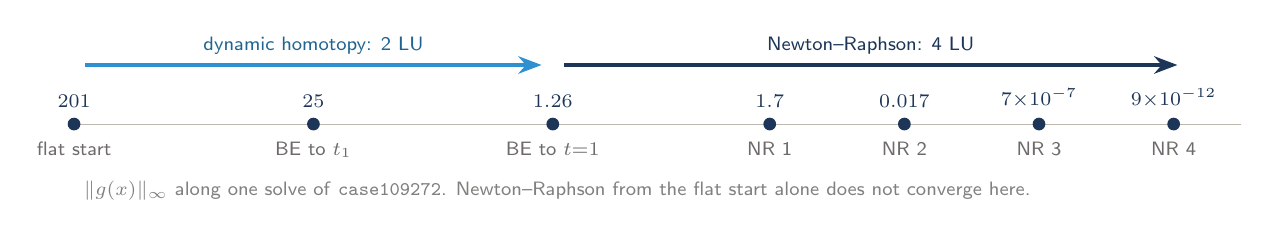
\begin{tikzpicture}[x=0.95cm,y=1cm]
  \draw[rulegrey] (0,0) -- (15.6,0);
  \foreach \x/\v/\lab in {0/201/flat start, 3.2/25/BE to $t_1$, 6.4/1.26/BE to $t{=}1$,
                          9.3/1.7/NR 1, 11.1/0.017/NR 2, 12.9/7{\times}10^{-7}/NR 3, 14.7/9{\times}10^{-12}/NR 4}{
    \fill[navy] (\x,0) circle (2.3pt);
    \node[font=\sffamily\scriptsize,text=ink!70,below] at (\x,-0.1) {\lab};
    \node[font=\sffamily\scriptsize,text=navy,above] at (\x,0.08) {$\v$};
  }
  \draw[skyblue,very thick,-{Stealth}] (0.15,0.75) -- node[above,font=\sffamily\scriptsize,text=skyblue!70!black]{dynamic homotopy: 2 LU} (6.25,0.75);
  \draw[navy,very thick,-{Stealth}] (6.55,0.75) -- node[above,font=\sffamily\scriptsize,text=navy]{Newton--Raphson: 4 LU} (14.75,0.75);
  \node[font=\sffamily\scriptsize,text=ink!60,anchor=west] at (0,-0.85) {$\|g(x)\|_\infty$ along one solve of \texttt{case109272}. Newton--Raphson from the flat start alone does not converge here.};
\end{tikzpicture}

\vfill
\begin{minipage}[t]{0.52\textwidth}
{\sffamily\bfseries\small\color{skyblue} SUBMITTED BY}\\[-4pt]
{\color{rulegrey}\rule{\linewidth}{0.5pt}}\\[2pt]
\begin{tabular}{@{}l@{\hspace{1.2em}}l@{}}
\Members
\end{tabular}
\end{minipage}\hfill
\begin{minipage}[t]{0.40\textwidth}
{\sffamily\bfseries\small\color{skyblue} SUBMITTED TO}\\[-4pt]
{\color{rulegrey}\rule{\linewidth}{0.5pt}}\\[2pt]
\textbf{\Supervisor}\\ \SupervisorRole\\[14pt]
{\sffamily\bfseries\small\color{skyblue} BASE PAPER}\\[-4pt]
{\color{rulegrey}\rule{\linewidth}{0.5pt}}\\[2pt]
{\small A.\ Lima-Silva and F.\,D.\ Freitas, \emph{Energies} 17(18):4642, 2024.}
\end{minipage}

\vspace{1.0cm}
\begin{center}
{\sffamily\small\color{ink!70} \SectionNo \quad\textbullet\quad \GroupNo \quad\textbullet\quad \ReportDate}
\end{center}
\restoregeometry
\end{titlepage}

% ============================================================================ ABSTRACT
\pagenumbering{roman}
\section*{Abstract}
\addcontentsline{toc}{section}{Abstract}
Newton--Raphson (NR) is the standard way to solve the power flow equations of an electrical grid, but on
large, badly conditioned networks it diverges when started from the usual \emph{flat start} (every voltage
at \SI{1}{pu}, every angle at zero). Lima-Silva and Freitas (2024) proposed a remedy: embed the equations
in a homotopy $G(x,t)=t\,g(x)+(1-t)K(x-\xo)$, turn it into an ordinary differential equation in $t$,
integrate that ODE with only two or three steps of backward Euler, and hand the rough result to NR or the
fast decoupled method. This report describes \textbf{DynHomotopy}, our Python implementation of that
method from first principles, and what we learned by pushing on it.

We rebuilt the complete pipeline (MATPOWER case reader, admittance matrix, polar power-flow equations
with an analytic Jacobian, NR, fast decoupled XB, the paper's three integrators and our reconstruction of
its static-homotopy baseline) and reproduced every table and figure of the paper. Of the 255 mismatch norms
printed in the paper's Tables 2--5, 246 agree with ours to within a factor of two, and 54 of the 63
iteration counts in its Table~7 agree exactly; the remaining differences trace back to eight
inconsistencies we found in the paper itself, which we document. We show algebraically that the
paper's recommended two-point backward-Euler path is a shifted (Levenberg--Marquardt-like) Newton step
followed by an almost plain Newton step, which explains both why it works and why explicit integrators
cannot.

We then added eight switchable modifications and tested 17 configurations on a test bed widened from the
paper's 9 systems to 34, under five parameter settings, for 2{,}890 runs, with cost counted in LU
factorizations rather than seconds. A run counts as solved only if it reaches the \emph{reference}
operating point: 14 of the 141 runs on which the paper's method converges land on a different root of the
power flow equations, so it truly solves 127 of 170. A Newton corrector after every path step raises this
to 152 with no losses and almost removes the wrong-root problem (2 runs instead of 14), for 5\% more
factorizations; combined with Iwamoto's optimal multiplier it keeps that robustness at 7\% \emph{fewer}
factorizations than the paper's method, which makes multiplier plus corrector our recommended configuration.
Richardson error control of the path steps is the only change that solves some systems nothing else solves,
at 18--30\% more factorizations. Four other ideas---a chord refinement of backward Euler that the paper itself
suggests, fixed-step RK4, a Jacobian-scaled homotopy and the standard Newton homotopy---make things worse,
and we explain why from the equations.

Finally we carried out the numerical studies stated in our proposal presentation: the spectrum of the flat-start Jacobian by
the power method and shifted inverse iteration, maps of where the method works in the $(K,\Delta t_0)$
plane, golden-section tuning of the shift $\delta=K/\Delta t_0$, and Gauss elimination and LU
factorization written from scratch. They show that $\delta$ matters only on the ill-conditioned grids,
that no simple spectral rule predicts it, and why a sparse direct solver is indispensable at this scale.

\clearpage
\tableofcontents
\clearpage
\listoffigures
\listoftables
\clearpage
\pagenumbering{arabic}

% ============================================================================ 1 INTRODUCTION
\section{Introduction}\label{sec:intro}

\subsection{The problem: finding where a grid settles}
Whenever an operator asks how the voltages across a network will settle for a given pattern of
generation and demand---before switching a line out, after a generator trips, while planning next
year's load---a \emph{power flow} problem is solved. For every bus $k$ the power injected by generators
minus the power drawn by loads has to equal the power flowing out through the lines, which gives two
nonlinear equations per bus in the unknown voltage magnitudes $V$ and angles $\theta$. Written compactly,
\begin{keyeq}
\[
  g(x) = 0, \qquad x = \bigl[\,\theta_{\mathrm{PV}},\ \theta_{\mathrm{PQ}},\ V_{\mathrm{PQ}}\,\bigr],
  \qquad g:\mathbb{R}^n\to\mathbb{R}^n,
\]
\end{keyeq}
where $n$ is 22 for the smallest system in this report and 185{,}807 for the largest.

The workhorse solver is Newton--Raphson (NR): linearise $g$ at the current point, solve the resulting
sparse linear system with one LU factorization, step, repeat. Near the solution it converges
quadratically, typically in three to six iterations. Far from the solution it has no guarantee at all.
And in practice it is usually started far away, from the \emph{flat start}: every magnitude at
\SI{1}{pu} and every angle at zero, because nothing better is known after a large disturbance or for a
network that has never been solved. On the five large, poorly conditioned grids of the base paper, NR from
the flat start does not converge on any of them (\cref{tab:systems}), even though a solution exists and
NR finds it easily from the stored operating point.

\subsection{Problem statement}
Lima-Silva and Freitas~\cite{lima2024} proposed to replace the flat start with a better one, computed
cheaply by following a homotopy from an easy problem to the real one with a very coarse numerical
integrator. Their paper reports that backward Euler with only two path points is enough for NR to converge
in four iterations on a 109{,}272-bus grid. This project set out to answer four questions:
\begin{enumerate}[label=\textbf{Q\arabic*.}]
  \item \textbf{Does it reproduce?} If we build the method ourselves, from the equations in the paper and
        nothing else, do we get the paper's numbers?
  \item \textbf{Why does it work?} The paper motivates the choice of backward Euler over forward Euler and
        RK2 mostly by experiment. Is there a reason visible in the algebra?
  \item \textbf{Is the paper internally consistent?} Where our numbers disagree, is the fault ours, or
        the paper's?
  \item \textbf{Can it be improved, and at what cost?} Which changes rescue systems the method fails on,
        which only make it faster, and which make it worse---measured on more systems than the paper uses,
        in a cost unit that does not depend on the computer, and counting a run as solved only if it
        reaches the right solution?
  \item \textbf{What do the numerics say about its parameters?} What does the spectrum of the flat-start
        Jacobian look like, where in the $(K,\Delta t_0)$ plane does the method work, and can the shift
        $\delta$ be tuned or predicted?
\end{enumerate}

\subsection{What we built}
\begin{itemize}
  \item \textbf{\code{dynhomotopy}}, a Python package that implements the full method from first
        principles: MATPOWER case files, the admittance matrix with taps and phase shifters, the polar
        power-flow equations with an analytic Jacobian checked against finite differences, NR, the XB
        fast decoupled method (FDXB), our reconstruction of the paper's static-homotopy baseline GSH-NR,
        the fixed-point homotopy with forward Euler, RK2 and backward Euler, and path schedules
        (\cref{sec:methods}).
  \item \textbf{A complete reproduction}: one script per table or figure of the paper, every output cell
        printed as \emph{ours / paper} (\cref{sec:repro}).
  \item \textbf{An audit} of eight places where the paper is inconsistent or under-specified
        (\cref{sec:audit}).
  \item \textbf{\code{improvements}}, a separate package of eight switchable modifications that never
        edits the reproduced code, and an evaluation of 17 configurations on 34 systems $\times$ 5
        settings with LU factorizations as the cost unit and a check that each run reaches the reference
        operating point (\cref{sec:mods,sec:modresults}).
  \item \textbf{The numerical studies} stated in our proposal presentation, in the same \code{improvements} package: power method and
        shifted inverse iteration for the Jacobian spectrum, $(K,\Delta t_0)$ feasibility maps,
        golden-section tuning of $\delta$, and Gauss elimination and LU with partial pivoting written from
        scratch (\cref{sec:proposal}).
  \item \textbf{A failure analysis} explaining from the equations why each unsuccessful modification
        fails (\cref{sec:failure}).
  \item \textbf{A command-line tool}, \code{python -m improvements}, that runs any modification or study
        on any of the 34 systems.
\end{itemize}

\begin{figure}[!htbp]
\centering
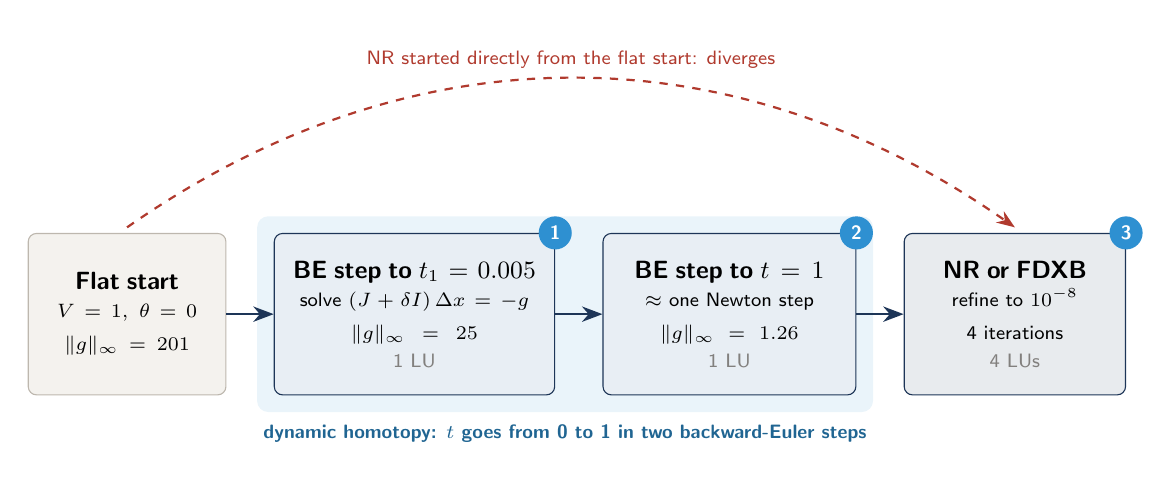
\begin{tikzpicture}[node distance=0.6cm,
  pipe/.style={draw=navy,fill=cloud,rounded corners=3pt,align=center,font=\sffamily\scriptsize,
    text width=#1,minimum height=2.05cm,inner sep=3pt}]
  \node[pipe=2.3cm,fill=mist,draw=rulegrey] (x0) {{\small\textbf{Flat start}}\\[2pt] $V=1,\ \theta=0$\\[4pt] $\ninf{g}=201$};
  \node[pipe=3.35cm,right=of x0] (s1) {{\small\textbf{BE step to $t_1=0.005$}}\\[2pt] solve $(J+\delta I)\,\Delta x=-g$\\[4pt] $\ninf{g}=25$\\[2pt] \textcolor{ink!60}{1 LU}};
  \node[pipe=3.0cm,right=of s1] (s2) {{\small\textbf{BE step to $t=1$}}\\[2pt] $\approx$ one Newton step\\[4pt] $\ninf{g}=1.26$\\[2pt] \textcolor{ink!60}{1 LU}};
  \node[pipe=2.6cm,right=of s2,fill=navy!10,draw=navy] (nr) {{\small\textbf{NR or FDXB}}\\[2pt] refine to $10^{-8}$\\[4pt] 4 iterations\\[2pt] \textcolor{ink!60}{4 LUs}};
  \draw[flow] (x0) -- (s1); \draw[flow] (s1) -- (s2); \draw[flow] (s2) -- (nr);
  \node[badge] at (s1.north east) {1}; \node[badge] at (s2.north east) {2}; \node[badge] at (nr.north east) {3};
  \draw[failred,thick,dashed,-{Stealth}] ([yshift=2pt]x0.north) to[out=35,in=145]
    node[pos=0.5,above,font=\sffamily\scriptsize,text=failred]{NR started directly from the flat start: diverges} ([yshift=2pt]nr.north);
  \begin{scope}[on background layer]
    \node[fill=skyblue!10,rounded corners=4pt,fit=(s1)(s2),inner sep=6pt] (hbox) {};
  \end{scope}
  \node[font=\sffamily\scriptsize\bfseries,text=skyblue!70!black,below=1pt of hbox] {dynamic homotopy: $t$ goes from 0 to 1 in two backward-Euler steps};
\end{tikzpicture}
\caption[The method of the base paper at a glance]{The method of the base paper at a glance, with the real
mismatch norms of one solve of \code{case109272} (\cref{fig:fig4}). Stage~\badgeref{1} regularises the
flat-start Jacobian by $\delta=K/\Delta t_0$; stage~\badgeref{2} is almost a plain Newton step; stage~\badgeref{3}
is ordinary NR from a much better starting point. \Cref{sec:firststep} derives both interpretations.}
\label{fig:pipeline}
\end{figure}

\subsection{Scope}
We treat steady-state AC power flow on transmission models in MATPOWER format, with the slack bus fixed
and generator reactive limits not enforced (MATPOWER's default, and the paper's setting). Distribution
networks, optimal power flow and contingency analysis are outside the scope. All reported experiments
solve their linear systems with SuperLU through SciPy~\cite{scipy,superlu}: the systems reach 185{,}807
unknowns and 1.4 million nonzeros. We also wrote Gauss elimination and LU with partial pivoting from
scratch and ran the paper's method with them on the systems up to 2{,}000 buses (\cref{sec:ownlu}); they
give the same iterates, and they show in numbers why a dense solver cannot be used on the large grids.
Run times are reported, but the primary cost measure is the number of LU factorizations, because our
Python timings are not comparable with the paper's MATLAB timings.

\subsection{How this report is organised}
\Cref{sec:background} reviews the power flow equations, NR, FDXB and homotopy methods, and the base paper's
claims. \Cref{sec:data} describes the 34 test systems. \Cref{sec:methods} presents the implementation and
derives what the first and last integration steps actually do. \Cref{sec:repro} reproduces the paper
result by result, and \cref{sec:audit} lists where the paper and our results disagree and why.
\Cref{sec:mods} introduces our eight modifications and the evaluation protocol, \cref{sec:modresults}
reports their results, \cref{sec:proposal} presents the numerical studies of the proposal, and
\cref{sec:failure} is a dedicated failure analysis. \Cref{sec:discussion,sec:conclusion} close with
discussion and conclusions; the appendices give reproduction commands and the full tables.


% ============================================================================ 2 BACKGROUND
\section{Background and the Base Paper}\label{sec:background}

\subsection{The power balance equations}
Let $Y = G + jB$ be the bus admittance matrix of the network and $V_k\angle\theta_k$ the voltage at bus
$k$. The active and reactive mismatch at bus $k$ are
\begin{align}
  \Delta P_k &= V_k \sum_{m} V_m\bigl(G_{km}\cos\theta_{km} + B_{km}\sin\theta_{km}\bigr) - P_k^{\mathrm{sp}}, \label{eq:p}\\
  \Delta Q_k &= V_k \sum_{m} V_m\bigl(G_{km}\sin\theta_{km} - B_{km}\cos\theta_{km}\bigr) - Q_k^{\mathrm{sp}}, \label{eq:q}
\end{align}
with $\theta_{km}=\theta_k-\theta_m$. Buses come in three types. At the single \emph{slack} bus $V$ and
$\theta$ are fixed. At \emph{PV} buses (generators) $P$ and $V$ are specified and $\theta$ is unknown.
At \emph{PQ} buses (loads) both $V$ and $\theta$ are unknown. Collecting the unknowns gives the state
$x=[\theta_{\mathrm{PV}},\theta_{\mathrm{PQ}},V_{\mathrm{PQ}}]\in\mathbb{R}^n$ with $n=N_{\mathrm{PV}}+2N_{\mathrm{PQ}}$,
and the equations $g(x)=[\Delta P_{\mathrm{PV}},\Delta P_{\mathrm{PQ}},\Delta Q_{\mathrm{PQ}}]=0$.
In complex form the whole mismatch vector is $\Delta S = V\circ\overline{(YV)} - S^{\mathrm{sp}}$, which is
how our implementation evaluates it (the same ordering and sign as MATPOWER~\cite{matpower}).

\subsection{Newton--Raphson and the fast decoupled method}
NR updates $x^{(i+1)} = x^{(i)} - J(x^{(i)})^{-1} g(x^{(i)})$, where $J=\partial g/\partial x$ is sparse
with the sparsity pattern of the network~\cite{tinney1967}. Each iteration costs one LU factorization of
$J$. The fast decoupled method~\cite{stott1974} approximates $J$ by two constant matrices,
\begin{equation}
  \Delta P / V = B'\,\Delta\theta, \qquad \Delta Q / V = B''\,\Delta V,
\end{equation}
factorised once and reused. In the XB variant~\cite{vanamerongen1989} used by the paper, resistances are
ignored only when building $B'$. FDXB iterations are cheap but many. The paper's Table~7 counts every
$P$--$\theta$ update and every $Q$--$V$ update as one iteration; MATPOWER's \code{fdpf} instead returns one
count per $P/Q$ cycle and only prints the $P$ and $Q$ counts separately.

\subsection{Homotopy methods}
A homotopy replaces the hard problem $g(x)=0$ by a family $G(x,t)=0$, $t\in[0,1]$, whose member at $t=0$
is trivial and whose member at $t=1$ is the real problem~\cite{watson1989,allgower2003}. A \emph{static}
homotopy picks points $0<t_1<\dots<t_N=1$ and solves $G(x,t_k)=0$ accurately at each one with NR, using
the previous solution as the start. The GSH-NR method of~\cite{freitas2022}, the baseline in the base
paper, is of this kind: it adds fictitious shunts that make the flat start an exact solution at $t=0$ and
removes them gradually. Its drawback is cost: every path point is a full NR solve.

A \emph{dynamic} homotopy~\cite{lima2024ijepes} instead differentiates $G(x(t),t)=0$ along the path,
\begin{equation}
  G_x\,\frac{dx}{dt} + G_t = 0
  \quad\Longrightarrow\quad
  \frac{dx}{dt} = -\,G_x(x,t)^{-1}\,G_t(x,t), \qquad x(0)=\xo, \label{eq:ode}
\end{equation}
and \emph{integrates} this ODE numerically, accepting that the result at $t=1$ is only approximate.
Continuous Newton methods~\cite{milano2009} are a close relative: they treat NR itself as the forward
Euler discretisation of an ODE.

\subsection{The base paper}\label{sec:basepaper}
Lima-Silva and Freitas~\cite{lima2024} use the fixed-point homotopy
\begin{keyeq}
\begin{equation}
  G(x,t) = t\,g(x) + (1-t)\,K\,(x-\xo), \label{eq:G}
\end{equation}
\end{keyeq}
whose derivatives are $G_x = t\,J(x)+(1-t)KI$ and $G_t = g(x)-K(x-\xo)$. The factor $K$, which earlier
work had set to one, is their main design lever. They integrate \eqref{eq:ode} with forward Euler (FE),
RK2 and a backward Euler (BE) scheme simplified to a single fixed-point iteration, always take the first
step to $t_1=\Delta t_0$ with BE, and refine the result at $t=1$ with NR or FDXB. On five ill-conditioned
grids built by replicating PEGASE networks~\cite{pegase} (18{,}482 to 109{,}272 buses) and four
loading-limit cases~\cite{tostado2019ill,tostado2019limit}, they report that:
\begin{itemize}
  \item FE and RK2 with large steps blow up on the big systems, while BE succeeds everywhere (their Tables 2--4);
  \item BE with just two path points, $\{0,\,0.005,\,1\}$, lets NR converge in four iterations where NR
        from the flat start fails (Table~7);
  \item BE followed by FDXB is faster than NR from the stored operating point, at 57--85\% of its CPU time (Table~8).
\end{itemize}
The paper's own future work mentions other homotopy functions and other integrators, which is where two
of our modifications come from.

\subsection{Related ideas we build on}
Iwamoto and Tamura~\cite{iwamoto1981} introduced the \emph{optimal multiplier}: scale each NR step by the
factor $\mu$ that minimises the mismatch along it, which for power flow in rectangular coordinates is an
exact quadratic. Predictor--corrector continuation~\cite{allgower2003} alternates a cheap predictor step
along the path with a Newton corrector back onto it. Adding a multiple of the identity to an
ill-conditioned Jacobian is the idea behind Levenberg--Marquardt damping~\cite{levenberg1944,marquardt1963},
and behind the conditioning step of~\cite{freitas2023}, which the base paper cites for its
$\delta I$ term. The implicit Euler method's stability on stiff problems is textbook
material~\cite{hairer1996}; \cref{sec:firststep} shows it is exactly what matters here.

% ============================================================================ 3 DATA
\section{Test Systems}\label{sec:data}

\subsection{Where the systems come from}
All systems are MATPOWER cases from two public Zenodo records by Tostado-V\'eliz, Kamel and Jurado,
the same files the paper uses: record 3514739 holds the \emph{ill-conditioned} systems~\cite{tostado2019ill},
built by gluing copies of European PEGASE and Polish networks together, and record 3491654 holds the
\emph{loading-limit} systems~\cite{tostado2019limit}, in which every load of a standard case was scaled up
until NR from a flat start was about to stop converging. Our code downloads each file on first use.

The paper uses nine of these systems. For the modification study we added every other system in the two
records that loads, giving 34: the paper's 5 ill-conditioned and 4 limit cases, 7 more ill-conditioned
systems and 18 more limit cases (\cref{tab:systems,fig:systems}). The wider test bed matters: 25 of the
34 systems were never seen while the paper's parameters were being chosen, so they test whether those
parameters generalise.

\begin{table}[p]
\centering
\caption[The 34 test systems]{The 34 test systems. $n$ is the number of unknowns, nnz the nonzeros of the
Jacobian at the flat start, and the last column the NR iterations needed from the flat start (limit 10).
The replicated construction of the ill-conditioned systems is from the dataset's own description.}
\label{tab:systems}
\footnotesize
\setlength{\tabcolsep}{4pt}
\begin{tabular}{@{}l l r r r r r r@{}}
\toprule
\headrow \thead{Case} & \thead{Built from} & \thead{Buses} & \thead{PV} & \thead{$n$} & \thead{nnz($J$)} & \thead{$\ninf{g(\xo)}$} & \thead{NR flat} \\
\midrule
\rows{generated/systems_rows.tex}
\bottomrule
\end{tabular}
\end{table}

\begin{figure}[!htbp]
\centering
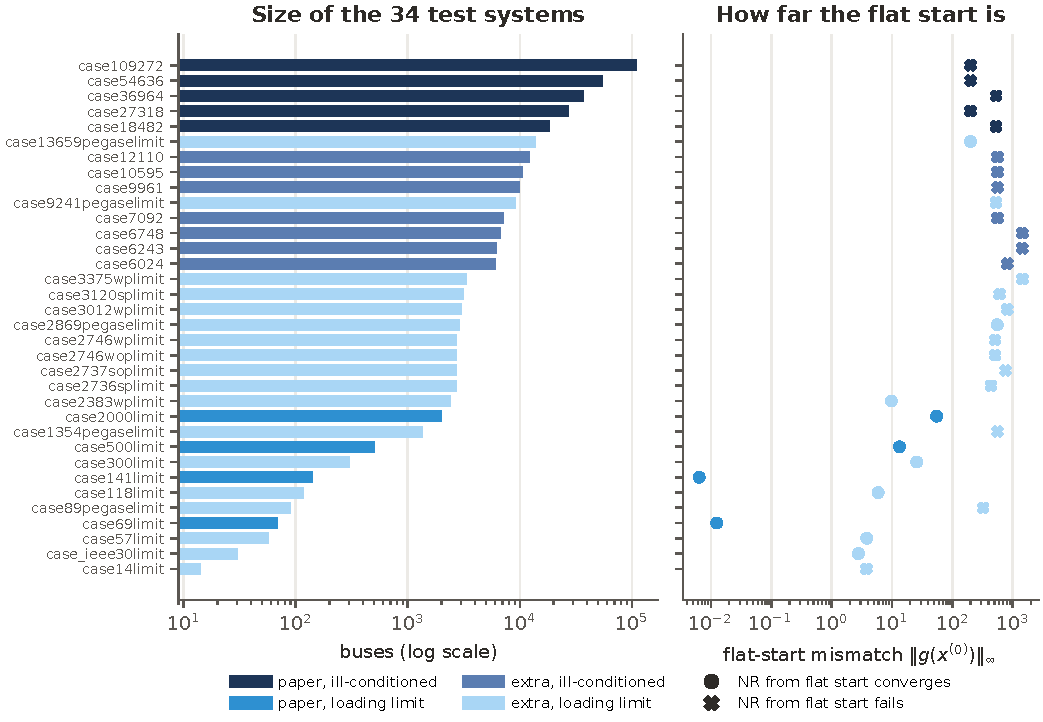
\includegraphics[width=\textwidth]{figures/systems.pdf}
\caption[Size and flat-start mismatch of the test systems]{Size and flat-start mismatch of all 34 test
systems, sorted by size. Size alone does not decide difficulty: NR from the flat start fails on the
14-bus limit case and succeeds on the 13{,}659-bus one. What the failing systems share is a large initial
mismatch---several hundred per unit on the ill-conditioned replicas.}
\label{fig:systems}
\end{figure}

\subsection{Structure of the Jacobian}
\Cref{fig:spy} shows the Jacobian at the flat start for three systems. The replicated construction is
directly visible: \code{case18482} is two copies of \code{case9241pegase}, and \code{case109272} is eight
copies of \code{case13659pegase}, each copy one diagonal block with only a few coupling entries between
them. Two consequences run through the rest of the report. First, the flat-start mismatch of a replica
equals that of its base network (533 for every 9241-based system, 201 for every 13659-based one). Second,
\code{case54636} and \code{case109272}, which are four and eight copies of the same network, behave
\emph{identically} in every experiment---they give the same norms to every printed digit. That identity
turns out to be a useful check on the paper (\cref{sec:audit}).

\begin{figure}[!htbp]
\centering
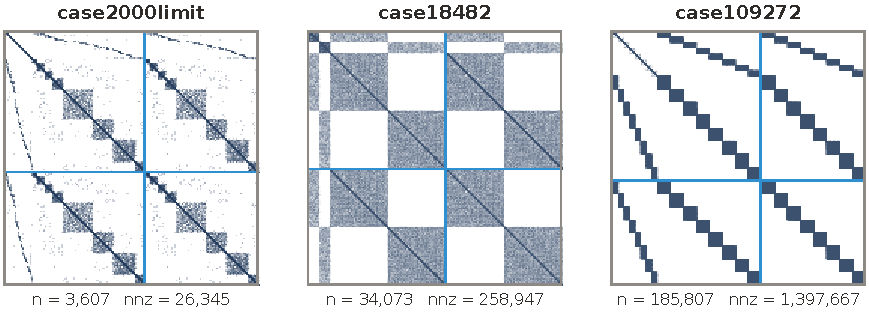
\includegraphics[width=\textwidth]{figures/spy.pdf}
\caption[Jacobian sparsity at the flat start]{Nonzero pattern of the Jacobian at the flat start. The orange
lines separate the angle unknowns from the voltage-magnitude unknowns, so each matrix shows the four blocks
$\partial P/\partial\theta$, $\partial P/\partial V$, $\partial Q/\partial\theta$, $\partial Q/\partial V$.
The ill-conditioned systems are copies of one network placed on the diagonal.}
\label{fig:spy}
\end{figure}

\subsection{Four details that change numbers}
\begin{description}[font=\sffamily\bfseries\color{navy},leftmargin=0pt,itemsep=3pt]
  \item[Base MVA of two limit cases.] \code{case69limit} and \code{case141limit} are stored with
        $\text{baseMVA}=10$. The paper's Tables 2--5 for these cases come out only on a \SI{100}{MVA}
        base, so every experiment uses 100 for them---but its NR-MAT and NR-flat counts in Table~7 match
        the stored 10. We return to this in \cref{sec:audit}.
  \item[The flat start includes the slack angle.] All angles, including the slack's, start at zero. For
        ``NR-MAT'' (NR from the operating point stored in the file) we shift the stored angles so the slack
        is at zero; both conventions lead to the same solution.
  \item[Many limit cases sit exactly on NR's budget.] Six of the 22 limit cases converge from the flat
        start in \emph{exactly} ten NR iterations, MATPOWER's default limit, and eleven more fail at ten.
        This is how the dataset was built, and it means any change worth one NR iteration can flip a limit
        case from failure to success. \Cref{sec:rescue} separates such cases from genuine rescues.
  \item[More than one solution.] The power flow equations have several roots, and a mismatch below
        $10^{-8}$ does not say which one was found. For every system we take as reference the solution NR
        reaches from the initial guess stored in the case file (up to 50 iterations, with the optimal
        multiplier as a fallback on the most stressed cases; \code{improvements.cases.reference\_voltage}).
        A run counts as \emph{solved} only if every bus voltage is within \SI{e-4}{pu} of the reference.
        This check changes the modification study substantially (\cref{sec:rootcheck}).
\end{description}

% ============================================================================ 4 METHODS
\section{Methods Implemented from the Base Paper}\label{sec:methods}

\subsection{Software architecture}
Everything in \code{dynhomotopy} is written against one small interface: a problem supplies $g(x)$ and
$J(x)$, and nothing else. The paper's $2\times2$ tutorial problem and the 109{,}272-bus grid therefore go
through exactly the same solver and integrator code. \Cref{fig:arch} shows the layers. Our
modifications live in a second package that imports the first and never edits it, so the reproduction
cannot be disturbed by later work; a test asserts that with every switch off, the modified solver returns
the paper's method bit for bit.

\begin{figure}[!htbp]
\centering
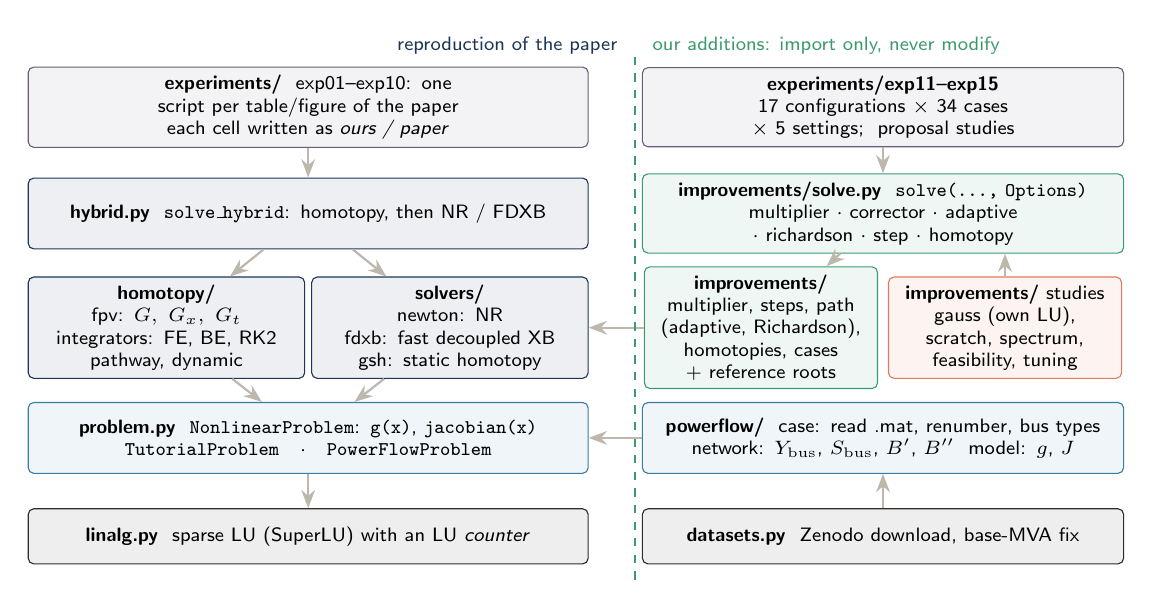
\begin{tikzpicture}[
  box/.style={draw=#1,fill=#1!8,rounded corners=2pt,font=\sffamily\scriptsize,align=center,inner sep=3pt,minimum height=0.9cm},
  lay/.style={font=\sffamily\scriptsize\bfseries,text=ink!60,anchor=east},
  x=1cm,y=1cm]
  % row 4: experiments
  \node[box=plum,text width=6.9cm] (exp) at (3.6,4.2) {\textbf{experiments/}\ \ exp01--exp10: one script per table/figure of the paper\\ each cell written as \emph{ours / paper}};
  \node[box=plum,text width=5.9cm] (exp11) at (10.9,4.2) {\textbf{experiments/exp11--exp15}\\ 17 configurations $\times$ 34 cases $\times$ 5 settings;\ \ proposal studies};
  % row 3: drivers
  \node[box=navy,text width=6.9cm] (hyb) at (3.6,2.85) {\textbf{hybrid.py}\ \ \code{solve\_hybrid}: homotopy, then NR / FDXB};
  \node[box=sage,text width=5.9cm] (imp) at (10.9,2.85) {\textbf{improvements/solve.py}\ \ \code{solve(..., Options)}\\ multiplier $\cdot$ corrector $\cdot$ adaptive $\cdot$ richardson $\cdot$ step $\cdot$ homotopy};
  % row 2: algorithms
  \node[box=navy,text width=3.3cm] (hom) at (1.8,1.4) {\textbf{homotopy/}\\ fpv: $G,\ G_x,\ G_t$\\ integrators: FE, BE, RK2\\ pathway, dynamic};
  \node[box=navy,text width=3.3cm] (sol) at (5.4,1.4) {\textbf{solvers/}\\ newton: NR\\ fdxb: fast decoupled XB\\ gsh: static homotopy};
  \node[box=sage,text width=2.75cm] (impm) at (9.35,1.4) {\textbf{improvements/}\\ multiplier, steps, path (adaptive, Richardson), homotopies, cases + reference roots};
  \node[box=coral,text width=2.75cm] (ext) at (12.45,1.4) {\textbf{improvements/} studies\\ gauss (own LU), scratch, spectrum, feasibility, tuning};
  % row 1: problem
  \node[box=sky,text width=6.9cm] (prob) at (3.6,0.0) {\textbf{problem.py}\ \ \code{NonlinearProblem}: \code{g(x)}, \code{jacobian(x)}\\ \code{TutorialProblem}\quad$\cdot$\quad \code{PowerFlowProblem}};
  \node[box=sky,text width=5.9cm] (pf) at (10.9,0.0) {\textbf{powerflow/}\ \ case: read .mat, renumber, bus types\\ network: $Y_{\mathrm{bus}}$, $S_{\mathrm{bus}}$, $B'$, $B''$\ \ model: $g$, $J$};
  % row 0: base
  \node[box=ink,text width=6.9cm,minimum height=0.7cm] (lin) at (3.6,-1.25) {\textbf{linalg.py}\ \ sparse LU (SuperLU) with an LU \emph{counter}};
  \node[box=ink,text width=5.9cm,minimum height=0.7cm] (ds) at (10.9,-1.25) {\textbf{datasets.py}\ \ Zenodo download, base-MVA fix};
  \foreach \a/\b in {exp/hyb,exp11/imp,hyb/hom,hyb/sol,imp/impm,hom/prob,sol/prob,prob/lin}
    \draw[-{Stealth},rulegrey,thick] (\a) -- (\b);
  \draw[-{Stealth},rulegrey,thick] (impm.west) -- (sol.east);
  \draw[-{Stealth},rulegrey,thick] (ext.north) -- (ext.north |- imp.south);
  \draw[-{Stealth},rulegrey,thick] (pf.west) -- (prob.east);
  \draw[-{Stealth},rulegrey,thick] (ds.north) -- (pf.south);
  \draw[sage,thick,dashed] (7.75,-1.8) -- (7.75,4.85);
  \node[font=\sffamily\scriptsize,text=sage,anchor=south west] at (7.85,4.75) {our additions: import only, never modify};
  \node[font=\sffamily\scriptsize,text=navy,anchor=south east] at (7.65,4.75) {reproduction of the paper};
\end{tikzpicture}
\caption[Architecture of the implementation]{Architecture of the implementation. Every solver sees only
$g(x)$ and $J(x)$; every LU factorization in the whole program goes through one counter, which is how
cost is measured in \cref{sec:modresults}.}
\label{fig:arch}
\end{figure}

\subsection{The homotopy and its three integrators}
The class \code{FixedPointHomotopy} implements \eqref{eq:G} and its derivatives in a few lines, and each
integration scheme is a function from $(x_k,t_k,\Delta t)$ to $x_{k+1}$. The listing below is the actual
code, lightly trimmed (Listing 1). With $\Phi(x,t) = -G_x(x,t)^{-1}G_t(x)$ the three schemes are
\begin{align}
  \text{FE:}\quad & x_{k+1} = x_k + \Delta t\,\Phi(x_k,t_k), \label{eq:fe}\\
  \text{RK2:}\quad & k_1=\Phi(x_k,t_k),\ \ k_2=\Phi(x_k+\Delta t\,k_1,\,t_{k+1}),\ \ x_{k+1}=x_k+\tfrac{\Delta t}{2}(k_1+k_2), \label{eq:rk2}\\
  \text{BE:}\quad & x_{k+1} = x_k + \Delta t\,\Phi(\hat x_{k+1},t_{k+1}),\quad \hat x_{k+1}=x_k \ \ \text{(one fixed-point iteration)}. \label{eq:be}
\end{align}
The implicit equation of true backward Euler, $x_{k+1}=x_k+\Delta t\,\Phi(x_{k+1},t_{k+1})$, is replaced by
one fixed-point iteration started at $x_k$, as in the paper. What remains ``implicit'' about BE is only
that it evaluates $G_x$ at the \emph{new} time $t_{k+1}$. That single detail is the whole story of the
next subsection.

\begin{codebox}{Listing 1 \quad The core of the method, from \texttt{homotopy/fpv.py} and \texttt{homotopy/integrators.py}}
\begin{lstlisting}[style=py]
class FixedPointHomotopy:              # G(x,t) = t g(x) + (1-t) K (x - x0)
    def G(self, x, t):
        return t * self.problem.g(x) + (1 - t) * self.K * (x - self.x0)
    def Gx(self, x, t):
        return (t * self.problem.jacobian(x) + (1 - t) * self.K * self.eye).tocsc()
    def Gt(self, x):
        return self.problem.g(x) - self.K * (x - self.x0)
    def dxdt(self, x, t):              # one sparse LU per call, counted
        return -solve(self.Gx(x, t), self.Gt(x), self.counter)

def forward_euler(h, x, t, dt):   return x + dt * h.dxdt(x, t)
def backward_euler(h, x, t, dt):  return x + dt * h.dxdt(x, t + dt)  # Gx at the NEW time
def runge_kutta2(h, x, t, dt):
    k1 = h.dxdt(x, t);  k2 = h.dxdt(x + dt * k1, t + dt)
    return x + dt / 2 * (k1 + k2)
\end{lstlisting}
\end{codebox}

\subsection{What the first step really does}\label{sec:firststep}
At $t_0=0$ the state is $\xo$, so $G_t = g(\xo)$ and the two schemes differ only in where they evaluate $G_x$.

\paragraph{Forward Euler} uses $G_x(\xo,0)=KI$: the network is invisible. The step is
\begin{equation}
  \Delta x_{\mathrm{FE}} = -\frac{\Delta t_0}{K}\,g(\xo) = -50\,g(\xo) \qquad(K=10^{-4},\ \Delta t_0=0.005).
\end{equation}
Every unknown is pushed by fifty times its own mismatch, and on the ill-conditioned systems the
mismatch is in the hundreds, so angles move by thousands of radians.

\paragraph{Backward Euler} uses $G_x(\xo,\Delta t_0) = \Delta t_0 J + (1-\Delta t_0)KI$, and the step becomes
\begin{keyeq}
\begin{equation}
\begin{aligned}
  \Delta x_{\mathrm{BE}} &= -\Delta t_0\bigl[\Delta t_0 J + (1-\Delta t_0)KI\bigr]^{-1} g(\xo)
    = -\bigl[J + \delta' I\bigr]^{-1} g(\xo),\\[2pt]
  \delta' &= \frac{(1-\Delta t_0)K}{\Delta t_0} \approx \frac{K}{\Delta t_0} = \delta = 0.02.
\end{aligned}\label{eq:shift}
\end{equation}
\end{keyeq}
This is a Newton step on $g$ with the Jacobian shifted by $\delta I$---structurally a Levenberg--Marquardt
step~\cite{levenberg1944,marquardt1963}. The paper derives the same expression (its eq.~25) and calls
$\delta$ a perturbation. The shift does two things. It keeps the linear system solvable where the
flat-start Jacobian is nearly singular, and it shortens the step in the directions where $J$ is weak,
which is exactly where a plain Newton step overshoots. The linearised static homotopy (the paper's eq.~27)
gives the same point, and our test suite checks the two agree to $10^{-10}$.

\begin{figure}[!htbp]
\centering
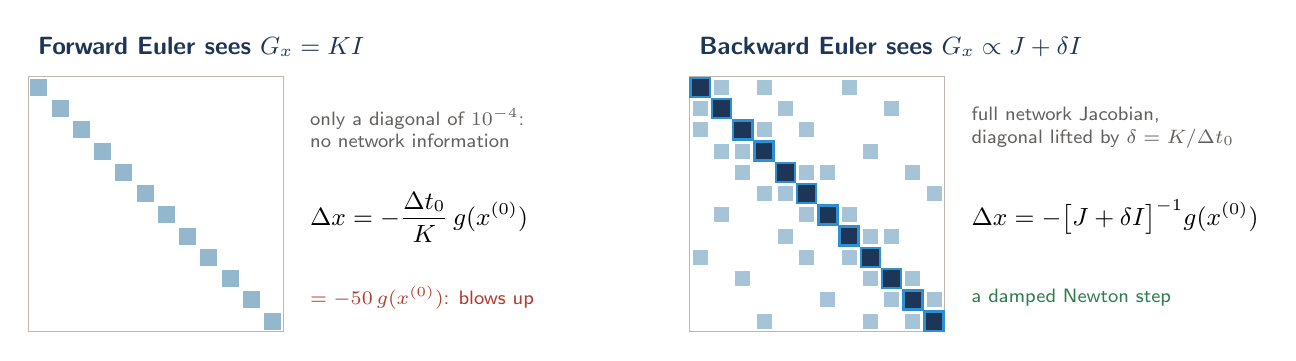
\begin{tikzpicture}[x=0.27cm,y=0.27cm]
  % FE panel
  \begin{scope}
    \node[font=\sffamily\small\bfseries,text=navy,anchor=west] at (0,13.4) {Forward Euler sees $G_x = K I$};
    \draw[rulegrey] (0,0) rectangle (12,12);
    \foreach \i in {0,...,11} \fill[sky!55] (\i+0.1,11.9-\i) rectangle (\i+0.9,11.1-\i);
    \node[font=\sffamily\scriptsize,text=ink!75,align=left,anchor=west] at (12.8,9.6) {only a diagonal of $10^{-4}$:\\ no network information};
    \node[font=\small,anchor=west] at (12.8,5.4) {$\Delta x = -\dfrac{\Delta t_0}{K}\,g(\xo)$};
    \node[font=\sffamily\scriptsize,text=failred,anchor=west] at (12.8,1.6) {$=-50\,g(\xo)$: blows up};
  \end{scope}
  % BE panel
  \begin{scope}[xshift=8.4cm]
    \node[font=\sffamily\small\bfseries,text=navy,anchor=west] at (0,13.4) {Backward Euler sees $G_x \propto J + \delta I$};
    \draw[rulegrey] (0,0) rectangle (12,12);
    \foreach \r/\c in {0/3,0/7,1/4,1/9,2/0,2/5,3/1,3/8,4/2,4/6,4/10,5/3,5/11,6/1,6/7,7/4,7/9,8/0,8/5,9/2,9/10,10/6,10/11,11/3,11/8,1/0,3/2,5/4,6/5,8/7,9/8,10/9,11/10,0/1,2/3,4/5,7/8,9/10,10/11}
      \fill[sky!45] (\c+0.15,11.85-\r) rectangle (\c+0.85,11.15-\r);
    \foreach \i in {0,...,11} \fill[navy] (\i+0.1,11.9-\i) rectangle (\i+0.9,11.1-\i);
    \foreach \i in {0,...,11} \draw[skyblue,line width=0.9pt] (\i+0.05,11.95-\i) rectangle (\i+0.95,11.05-\i);
    \node[font=\sffamily\scriptsize,text=ink!75,align=left,anchor=west] at (12.8,9.6) {full network Jacobian,\\ diagonal lifted by $\delta=K/\Delta t_0$};
    \node[font=\small,anchor=west] at (12.8,5.4) {$\Delta x = -\bigl[J+\delta I\bigr]^{-1} g(\xo)$};
    \node[font=\sffamily\scriptsize,text=okgreen,anchor=west] at (12.8,1.6) {a damped Newton step};
  \end{scope}
\end{tikzpicture}
\caption[What each integrator sees on the first step]{What each integrator ``sees'' on the first step. The
matrix that forward Euler inverts at $t=0$ is $KI$, so its step ignores the network entirely; backward Euler
evaluates $G_x$ one step later, where it is proportional to the real Jacobian plus a small diagonal shift.}
\label{fig:firststep-diagram}
\end{figure}

\paragraph{The last step is almost Newton.} The paper's favourite path has only one more point, $t=1$.
With BE, $G_x$ is evaluated at $t=1$, where $G_x = J(x_1)$ and $K$ disappears from it:
\begin{equation}
  x(1) = x_1 - (1-\Delta t_0)\,J(x_1)^{-1}\bigl[g(x_1) - K(x_1-\xo)\bigr]
       \approx x_1 - J(x_1)^{-1} g(x_1).
\end{equation}
The factor $0.995$ and the term $K(x_1-\xo)$, with $K=10^{-4}$, are tiny. So the two-point BE ``homotopy''
is one shifted Newton step followed by an almost plain Newton step, after which NR proper takes over.
This explains three things the paper reports. Its cost is essentially that of NR (two LUs for the path,
then 3--4 for NR). The regularising work happens entirely in the first step, which is why $\delta$, not
$K$ or $\Delta t_0$ alone, is the parameter that matters. And explicit schemes cannot compete with a
large final step, because at $t=1$ they would have to use $G_x$ evaluated at the previous, smaller $t$.

\begin{figure}[!htbp]
\centering
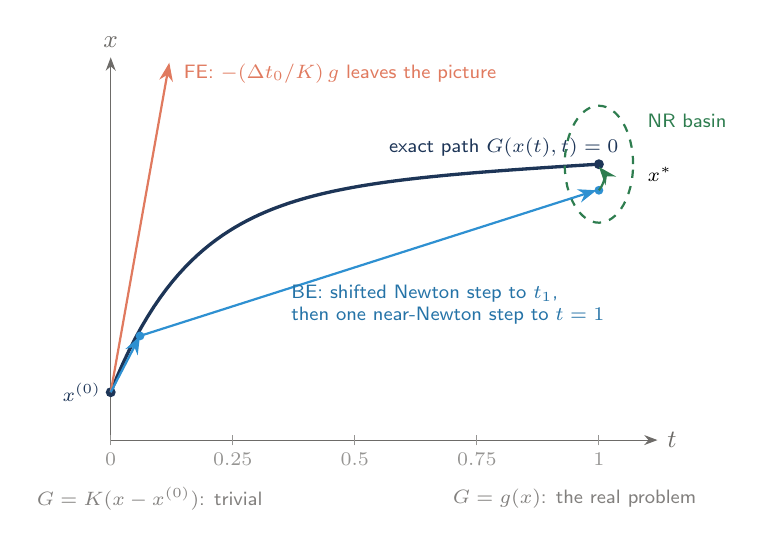
\begin{tikzpicture}[x=6.2cm,y=1.35cm]
  \draw[-{Stealth},ink!70] (0,-0.2) -- (1.12,-0.2) node[right,font=\small]{$t$};
  \draw[-{Stealth},ink!70] (0,-0.2) -- (0,3.4) node[above,font=\small]{$x$};
  \foreach \t in {0,0.25,0.5,0.75,1} \draw[ink!50] (\t,-0.25) -- (\t,-0.15) node[below=3pt,font=\scriptsize]{\t};
  % exact path
  \draw[navy,very thick,domain=0:1,samples=80] plot (\x,{0.25+1.9*(1-exp(-6*\x))+0.25*\x});
  \node[font=\sffamily\scriptsize,text=navy,anchor=west] at (0.55,2.55) {exact path $G(x(t),t)=0$};
  \fill[navy] (0,0.25) circle (1.8pt) node[left,font=\scriptsize]{$\xo$};
  \fill[navy] (1,2.395) circle (1.8pt);
  % NR basin
  \draw[okgreen,dashed,thick] (1,2.395) ellipse (0.07 and 0.55);
  \node[font=\sffamily\scriptsize,text=okgreen,anchor=west] at (1.08,2.8) {NR basin};
  \node[font=\scriptsize,anchor=west] at (1.08,2.3) {$x^\ast$};
  % FE first step
  \draw[coral,thick,-{Stealth}] (0,0.25) -- (0.12,3.35);
  \node[font=\sffamily\scriptsize,text=coral,anchor=west,align=left] at (0.13,3.25) {FE: $-(\Delta t_0/K)\,g$ leaves the picture};
  % BE steps
  \draw[skyblue,thick,-{Stealth}] (0,0.25) -- (0.06,0.78);
  \fill[skyblue] (0.06,0.78) circle (1.6pt);
  \draw[skyblue,thick,-{Stealth}] (0.06,0.78) -- (0.995,2.15);
  \fill[skyblue] (1,2.15) circle (1.6pt);
  \node[font=\sffamily\scriptsize,text=skyblue!80!black,anchor=north west,align=left] at (0.35,1.35) {BE: shifted Newton step to $t_1$,\\ then one near-Newton step to $t=1$};
  \draw[okgreen,thick,-{Stealth}] (1,2.15) to[bend right=40] (1.0,2.37);
  \node[font=\sffamily\scriptsize,text=ink!60] at (0.08,-0.75) {$G=K(x-\xo)$: trivial};
  \node[font=\sffamily\scriptsize,text=ink!60] at (0.95,-0.75) {$G=g(x)$: the real problem};
\end{tikzpicture}
\caption[Geometry of the dynamic homotopy]{Schematic of the dynamic homotopy. BE does not track the path
closely---it only needs to land inside the region from which NR converges. A real two-dimensional
instance of this picture, computed with our code, is \cref{fig:tutorial}.}
\label{fig:homotopy-sketch}
\end{figure}

\subsection{The refining solvers}
\paragraph{NR} (\code{solvers/newton.py}) stops when $\ninf{g}<10^{-8}$ or after 10 iterations,
MATPOWER's defaults and the paper's setting. A singular Jacobian or a non-finite mismatch ends the run as
a failure.

\paragraph{FDXB} (\code{solvers/fdxb.py}) follows MATPOWER's \code{fdpf}: $B'$ ignores shunts, line
charging, taps and resistance; $B''$ keeps the full network without phase shifters; both are factorised
once. Each iteration is a $P$--$\theta$ update followed by a $Q$--$V$ update. We report the number of
$P$ updates plus $Q$ updates, because that is what the paper's Table~7 counts (for example $15+14=29$);
this is not \code{fdpf}'s return value, which counts $P/Q$ cycles.

\paragraph{GSH-NR} (\code{solvers/gsh.py}) is the paper's static-homotopy baseline from~\cite{freitas2022}.
The paper describes it only in words, so ours is a reconstruction: fictitious shunts sized to make the
flat start an exact solution at $h=0$ and scaled by $(1-h)$, and the impedance of branches at the slack bus
multiplied by $\delta+(1-\delta)h$; $h$ runs from $\Delta h$ to 1 and every point is a full NR solve. Where
our version and the paper's differ is recorded in \cref{sec:audit}.

\begin{algo}{Algorithm 1 \quad The base paper's hybrid method (as implemented in \texttt{hybrid.py})}
\begin{algorithmic}[1]
\Require problem $(g,J)$, flat start $\xo$, factor $K$, time points $0=t_0<t_1<\dots<t_N=1$, scheme $\in\{\mathrm{FE},\mathrm{RK2},\mathrm{BE}\}$
\State $x \gets \xo$
\For{$k = 0,\dots,N-1$}
  \State $\Delta t \gets t_{k+1}-t_k$;\quad \textbf{if} $k=0$ \textbf{then} use BE \textbf{else} use the chosen scheme
  \State $x \gets \textsc{Step}(x,t_k,\Delta t)$ \Comment{each $\Phi$ evaluation = one sparse LU}
  \If{a matrix is singular \textbf{or} $\ninf{g(x)}$ is not finite} \Return failure \EndIf
\EndFor
\State \Return $\textsc{NR}(x)$ or $\textsc{FDXB}(x)$ \Comment{the refiner starts from $\hat x^{(0)} = x(1)$}
\end{algorithmic}
\end{algo}

\subsection{Verification before measurement}
Before any number was compared with the paper, the building blocks were tested on their own
(\code{tests/}, 24 tests, all passing):
\begin{itemize}
  \item the analytic Jacobian agrees with central finite differences on two real systems;
  \item the path generator produces the paper's time grids, including the shortened last step;
  \item the BE first step and the linearised static homotopy (the paper's eqs.~25 and 27) give the same point;
  \item NR on the tutorial takes exactly 11 iterations to the root $(1.5,0.5)$ from $x_2^{(0)}=0.995$, as in the paper's Fig.~1(a);
  \item NR-MAT and NR-flat iteration counts, one full row of Table~4 and the FDXB count of Table~7 for \code{case2000limit} match the paper;
  \item with every modification switched off, the modified solver returns the paper's method exactly;
  \item our Gauss elimination and LU agree with NumPy, pivot past a zero diagonal, and give the same
        Newton iterates as SuperLU on \code{case500limit};
  \item the power method and shifted inverse iteration find the known eigenvalues of a diagonal matrix,
        and golden-section search finds the minimum of a parabola;
  \item Richardson step control reaches $t=1$ and converges, and both command-line tools run.
\end{itemize}

% ============================================================================ 5 REPRODUCTION
\section{Reproducing the Base Paper}\label{sec:repro}

Each of the paper's results has its own script in \code{experiments/} (\cref{tab:scripts} in the appendix).
Every table cell below is shown as our value above the paper's value.

\subsection{The two-variable tutorial}
The paper first tests the idea on $g_1=x_1^2+x_2^2-2x_1x_2-1$, $g_2=x_1+x_2-2$ from $\xo=(1,1)$, where the
Jacobian is singular. The system has two roots, $A=(1.5,0.5)$ and $B=(0.5,1.5)$, and the singular set is the
whole line $x_1=x_2$ through the starting point. \Cref{fig:tutorial} draws what the three integrators
actually do in this plane, which the paper only shows as mismatch curves. The exact homotopy path (traced
with 800 corrected steps) bends from $\xo$ to root $A$. With $K=0.05$ all three coarse integrators stay
near it; with $K=0.005$ the explicit ones overshoot across the singular line and NR then converges to
root $B$, while BE stays on the right side and reaches $A$.

\begin{figure}[!htbp]
\centering
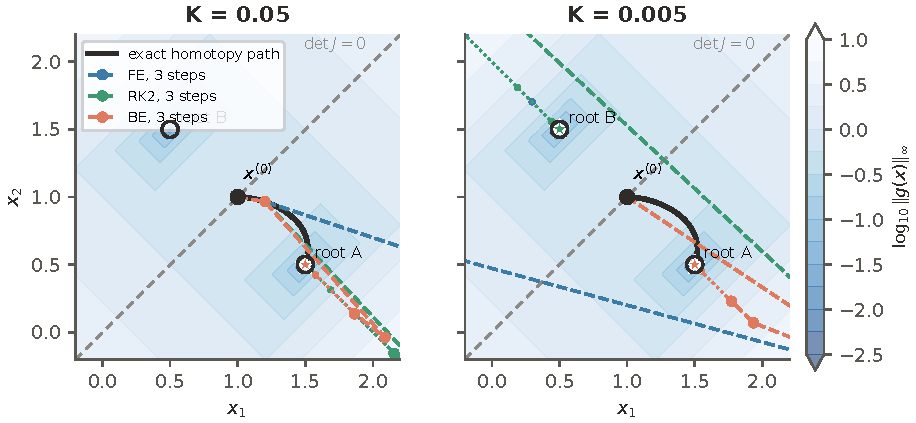
\includegraphics[width=\textwidth]{figures/tutorial_geometry.pdf}
\caption[The tutorial problem in the plane]{The tutorial problem in the $(x_1,x_2)$ plane, $\Delta t_0=0.01$
then $\Delta t=0.5$. Background: $\log_{10}\ninf{g}$. Black: the exact homotopy path. Dashed: the three
coarse integrations; dotted: the NR iterations that follow; stars: where NR ends. At the smaller $K$ the
explicit schemes cross the singular line $\det J=0$ and NR finds the other root.}
\label{fig:tutorial}
\end{figure}

\Cref{fig:tut-repro} and \cref{tab:tutorial} compare iteration counts. NR alone matches the paper for
$\epsilon=0.005$ and $0.01$ (11 and 10 iterations); for $\epsilon=0.05$ we need 8, not 9, and we show in
\cref{sec:audit} that the paper's curve for that case cannot come from these equations. In the hybrid runs
BE is the best start for NR in every panel, as in the paper, but some counts differ by one or two.

\begin{figure}[p]
\centering
\begin{subfigure}{0.49\textwidth}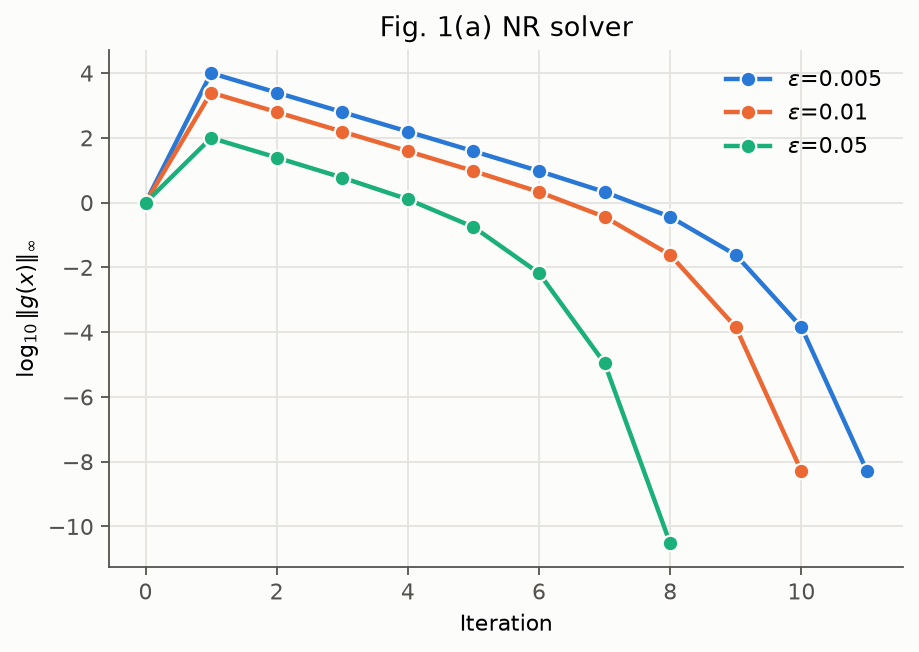
\includegraphics[width=\linewidth]{figures/repo/fig1a_tutorial_nr.png}\caption{Fig.~1(a): NR alone from $(1,1-\epsilon)$}\end{subfigure}\hfill
\begin{subfigure}{0.49\textwidth}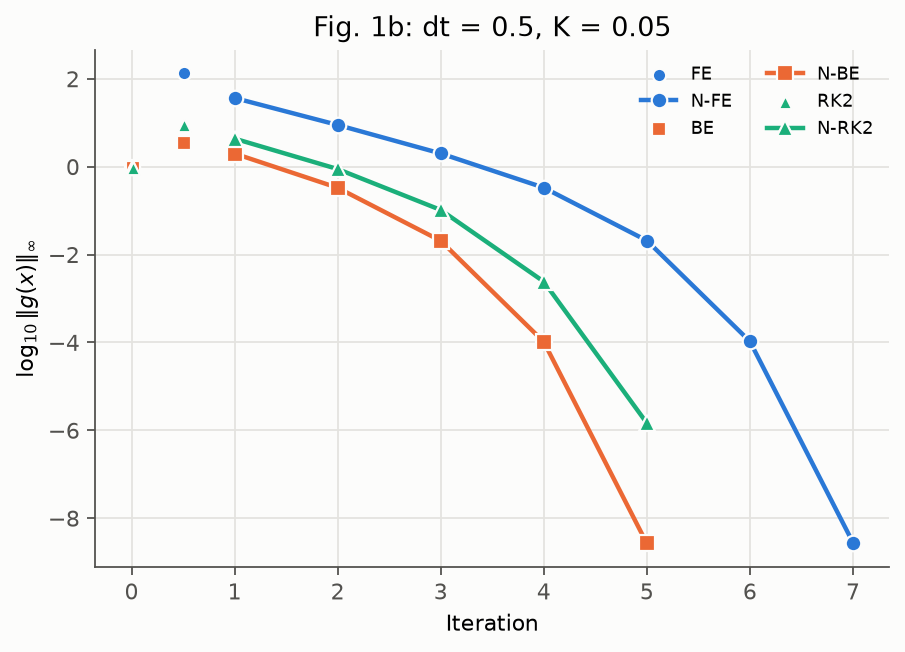
\includegraphics[width=\linewidth]{figures/repo/fig1b_tutorial_hybrid.png}\caption{Fig.~1(b): homotopy then NR, $\Delta t=0.5$, $K=0.05$}\end{subfigure}\\[6pt]
\begin{subfigure}{0.49\textwidth}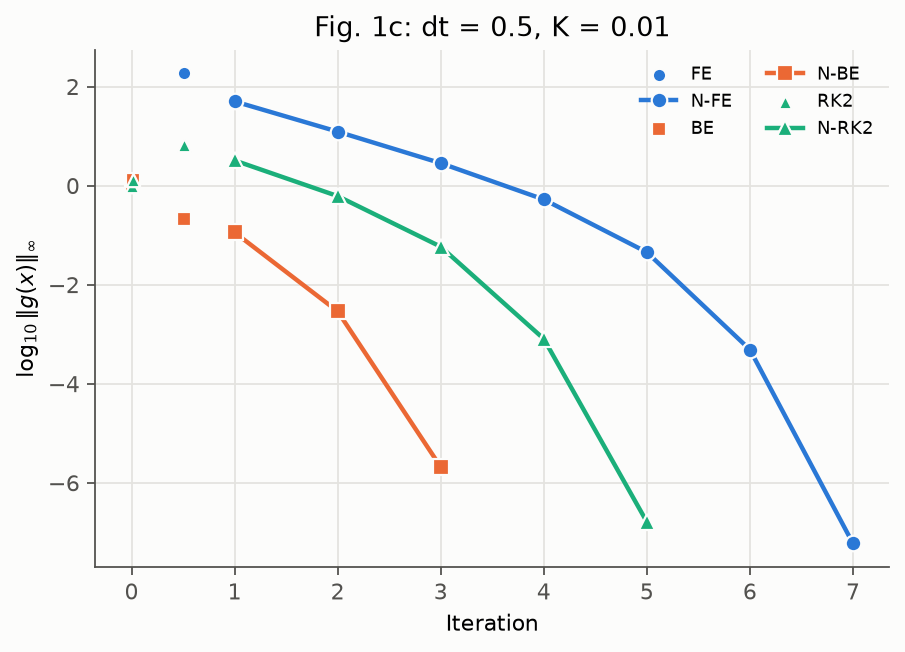
\includegraphics[width=\linewidth]{figures/repo/fig1c_tutorial_hybrid.png}\caption{Fig.~1(c): $\Delta t=0.5$, $K=0.01$}\end{subfigure}\hfill
\begin{subfigure}{0.49\textwidth}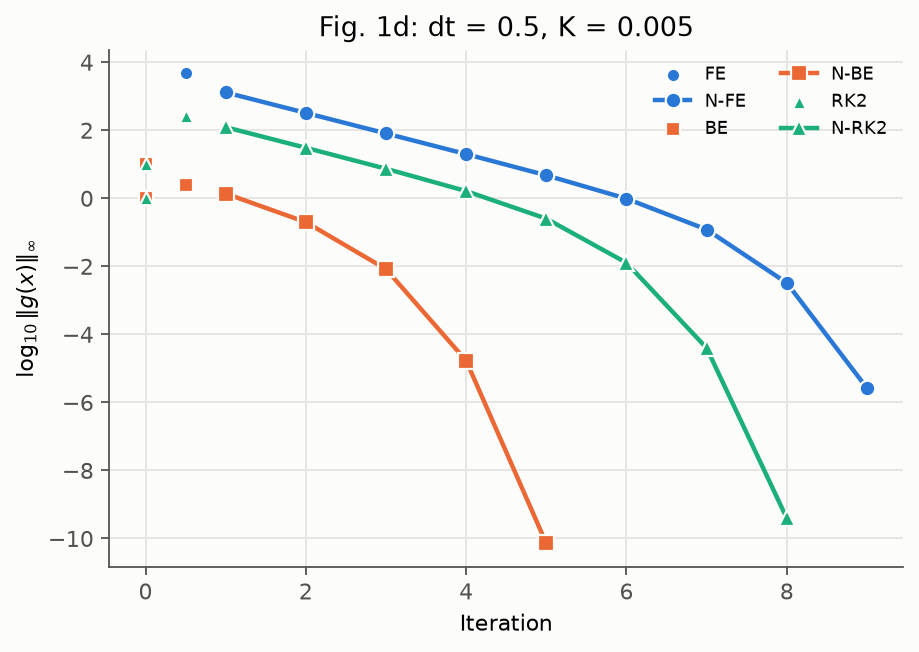
\includegraphics[width=\linewidth]{figures/repo/fig1d_tutorial_hybrid.png}\caption{Fig.~1(d): $\Delta t=0.5$, $K=0.005$}\end{subfigure}\\[6pt]
\begin{subfigure}{0.49\textwidth}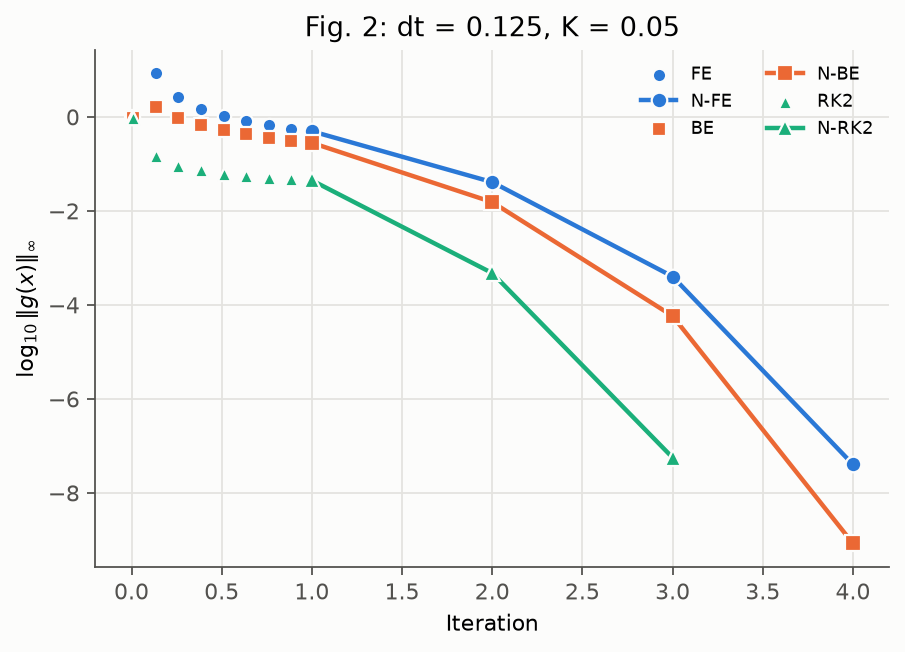
\includegraphics[width=\linewidth]{figures/repo/fig2_tutorial_hybrid.png}\caption{Fig.~2: smaller step $\Delta t=0.125$, $K=0.05$}\end{subfigure}\hfill
\begin{minipage}[b]{0.47\textwidth}\small
\textbf{Reading the panels.} Scattered markers are the homotopy points, drawn at their time
$t\in[0,1]$; the connected curves are the NR iterations that follow, iteration $i$ drawn at $1+i$.
Orange squares (BE) reach $10^{-5}$ first in every hybrid panel, as in the paper. In (c) and (d) the FE
and RK2 runs converge, but to root $B$ rather than $A$ (\cref{fig:tutorial}). With the smaller step of
panel (e) all three schemes give NR a good start.
\vspace{1.2cm}
\end{minipage}
\caption[Tutorial: our versions of the paper's Figures 1 and 2]{Our versions of all five tutorial panels
of the paper (Figures 1(a)--(d) and 2), generated by \code{exp01\_tutorial.py}.}
\label{fig:tut-repro}
\end{figure}

\begin{table}[!htbp]
\centering
\caption[Tutorial: NR iterations after each start]{Tutorial: NR iterations to $\ninf{g}<10^{-5}$, ours and
read off the paper's plots, and the root reached.}
\label{tab:tutorial}
\small
\begin{tabular}{@{}l c c r r c@{}}
\toprule
\headrow \thead{Run} & \thead{$\Delta t$} & \thead{$K$} & \thead{Ours} & \thead{Paper} & \thead{Root} \\
\midrule
NR only, $\epsilon=0.005$ & -- & -- & 11 & 11 & $A$ \\
NR only, $\epsilon=0.01$ & -- & -- & 10 & 10 & $A$ \\
NR only, $\epsilon=0.05$ & -- & -- & 8 & 9 & $A$ \\
\midrule
FE / BE / RK2 then NR & 0.5 & 0.05 & 6 / 4 / 4 & 6 / 3 / 6 & $A$ / $A$ / $A$ \\
FE / BE / RK2 then NR & 0.5 & 0.01 & 6 / 2 / 4 & 4 / 2 / 4 & $B$ / $A$ / $B$ \\
FE / BE / RK2 then NR & 0.5 & 0.005 & 8 / 4 / 7 & 6 / 3 / 7 & $B$ / $A$ / $B$ \\
FE / BE / RK2 then NR & 0.125 & 0.05 & 3 / 3 / 2 & 3 / 2 / 3 & $A$ / $A$ / $A$ \\
\bottomrule
\end{tabular}
\end{table}

\subsection{The first time step}
Section 4.2.1 of the paper argues that explicit schemes cannot take the first step. \Cref{fig:first}
measures it on all nine systems: FE multiplies the mismatch by factors between $7\times10^{3}$ and
$1.8\times10^{10}$; RK2, which evaluates a second slope at the FE point, does no better; BE reduces the
mismatch by roughly a factor of eight on every ill-conditioned system (533 to 65, 201 to 25), exactly the
paper's numbers. Taking the explicit step with $K=1$ instead, the value earlier work used, avoids the
explosion but moves the state so little that nothing is gained.

\begin{figure}[!htbp]
\centering
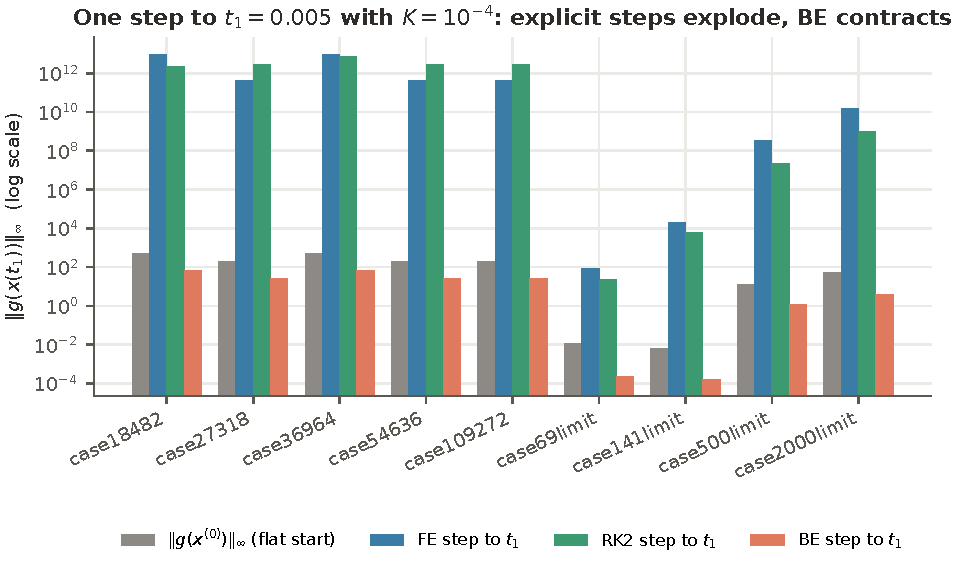
\includegraphics[width=0.93\textwidth]{figures/first_step.pdf}
\caption[First step: explicit schemes explode]{Mismatch after the single first step to $t_1=0.005$,
$K=10^{-4}$ (log scale). Grey is the flat start. Forward Euler and RK2 make every system worse by orders of
magnitude; backward Euler improves every one.}
\label{fig:first}
\end{figure}

\subsection{Tables 2--4: one large step after $t_2$}
The paper's Tables 2--4 use the path $\{0,\,0.005,\,0.01,\,0.51,\,1\}$ with $K=10^{-4}$: BE to $t_1$, then
the scheme under test with a large step. \Cref{tab:be} shows the BE results: they match the paper almost
digit for digit, including the three NR iterations that follow. For \code{case18482} we get 533, 65, 33,
7.2, 3.7 along the path and 0.042, $1.5\times10^{-5}$, $7.7\times10^{-12}$ in NR, against the paper's 532,
65, 33, 7.2, 3.7 and 0.04, $1.5\times10^{-5}$, $10^{-11}$. The FE and RK2 tables (\cref{app:tables}) match
wherever the schemes stay finite; where they blow up, they blow up at the same point but not to the same
size, which is expected once a number is $10^{9}$ or more and is dominated by rounding.

\begin{table}[!htbp]
\centering
\caption[Table 4 re-run: BE then NR]{Table 4 re-run: $\ninf{g}$ along the BE path $\{0,0.005,0.01,0.51,1\}$
and after each of the first three NR iterations, $K=10^{-4}$. Each case shows our value above the paper's.}
\label{tab:be}
\scriptsize
\setlength{\tabcolsep}{3.3pt}
\begin{tabular}{@{}l l r r r r r r r r l@{}}
\toprule
\headrow \thead{Case} & & \thead{$t{=}0$} & \thead{0.005} & \thead{0.01} & \thead{0.51} & \thead{1} & \thead{NR 1} & \thead{NR 2} & \thead{NR 3} & \thead{Result} \\
\midrule
\rows{generated/table4_rows.tex}
\bottomrule
\end{tabular}
\end{table}

\subsection{Table 5: growing steps}
Table 5 of the paper uses, on three systems, a path whose steps grow geometrically:
\[
  \{0,\ 0.005,\ 0.01,\ 0.02,\ 0.12,\ 0.62,\ 1\}.
\] With more points, all three schemes give NR a usable start, although after FE the
NR stage needs five iterations instead of three on both \code{case36964} and \code{case2000limit}. All of our cells
that carry a number (89 of the 90; one is blank in both) agree with the paper's to within a factor of two
(\cref{tab:t5,fig:fidelity}).

\begin{table}[!htbp]
\centering
\caption[Table 5 re-run: growing time steps]{Table 5 re-run, $K=10^{-4}$: $\ninf{g}$ at each path point and
after three NR iterations.}
\label{tab:t5}
\scriptsize
\setlength{\tabcolsep}{2.6pt}
\begin{tabular}{@{}l l l r r r r r r r r r r@{}}
\toprule
\headrow \thead{Case} & \thead{Solver} & & \thead{$t{=}0$} & \thead{0.005} & \thead{0.01} & \thead{0.02} & \thead{0.12} & \thead{0.62} & \thead{1} & \thead{NR 1} & \thead{NR 2} & \thead{NR 3} \\
\midrule
\rows{generated/table5_rows.tex}
\bottomrule
\end{tabular}
\end{table}

\subsection{How close is the reproduction, overall?}
\Cref{fig:fidelity} puts every numeric cell of Tables 2--5 on one plot: 255 pairs of (paper, ours). 246
of them (96\%) agree within a factor of two, and 199 (78\%) within 10\%, which is the rounding of the
paper's two printed digits. Of the nine outliers, seven are divergent FE and RK2 values above $10^{3}$,
one is the Table 2 cell discussed in \cref{sec:audit}, and one is a final NR mismatch near $10^{-11}$, at
rounding level.

\begin{figure}[!htbp]
\centering
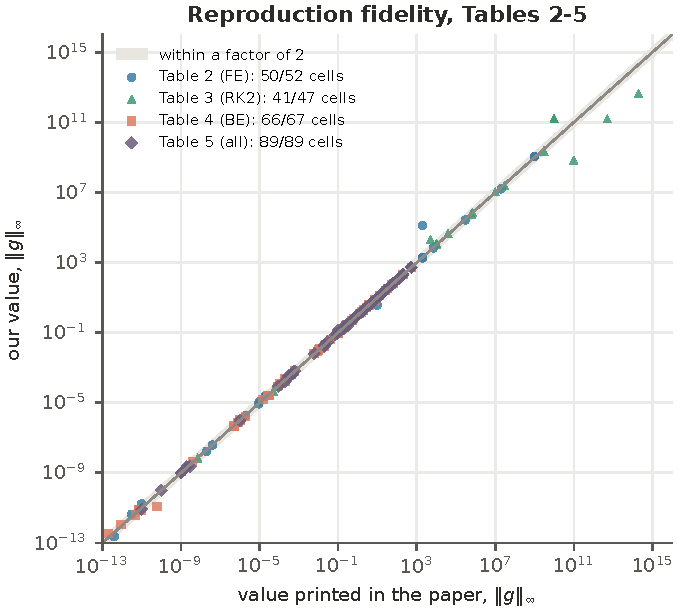
\includegraphics[width=0.6\textwidth]{figures/fidelity.pdf}
\caption[Reproduction fidelity across Tables 2--5]{Every numeric cell of the paper's Tables 2--5 against
our value, on log axes spanning 28 orders of magnitude. The grey band is agreement within a factor of two.}
\label{fig:fidelity}
\end{figure}

\subsection{Section 4.4: larger first steps}
Section 4.4 of the paper raises $\Delta t_0$ to 0.05 and $K$ to 0.001, keeping $\delta=0.02$, and tries
paths of three, four and five points. It reports that with few points only BE works, and that raising
$\Delta t_0$ further to 0.1 (with $K=0.002$) fails. \Cref{fig:sec44} is our full grid. BE gives NR a usable
start in 75 of 81 (path, system) cells, FE in 64 and RK2 in 59. On three-point paths BE works on 8 of 9
systems and FE and RK2 on only 3, confirming the paper's main claim. Two details disagree: FE and RK2
also succeed on several four-point paths, and BE followed by NR fails on \code{case36964} with only three
points (FDXB still converges). And for $\Delta t_0=0.1$ the picture depends on the path, which the paper does
not give: the three-point path works on eight systems, the five-point path $\{0,0.1,0.2,0.3,1\}$ fails with
NR on the four largest.

\begin{figure}[!htbp]
\centering
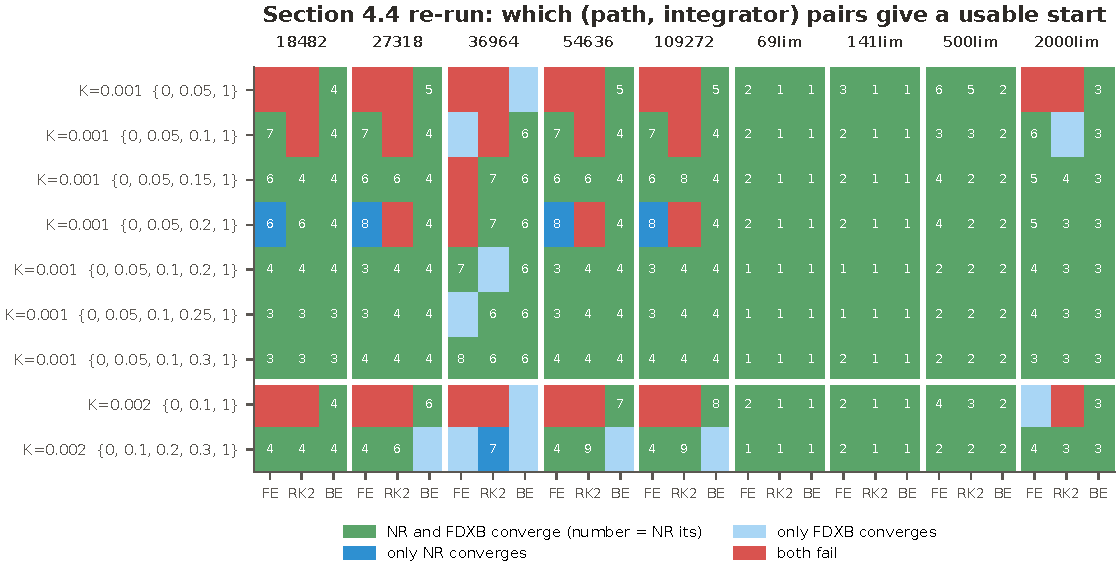
\includegraphics[width=\textwidth]{figures/sec44_grid.pdf}
\caption[Section 4.4 re-run: which paths give a usable start]{Section 4.4 re-run. Rows: paths and $K$;
columns: system and scheme. Colour: whether NR and FDXB converge afterwards; number: NR iterations.}
\label{fig:sec44}
\end{figure}

\subsection{Figure 3 and Table 6: five-point paths}
With five-point paths $\{0,0.05,0.1,t_3,1\}$ and $K=0.001$, \cref{fig:fig3} reproduces the paper's Figure 3,
including its one failure: FE with $t_3=0.25$ on \code{case36964}. We find one more: RK2 with $t_3=0.20$ on
the same system diverges in our run (the dotted green line leaving panel a), where the paper reports a
successful solve at 232\% of the NR-MAT time.

\begin{figure}[!htbp]
\centering
\begin{subfigure}{0.325\textwidth}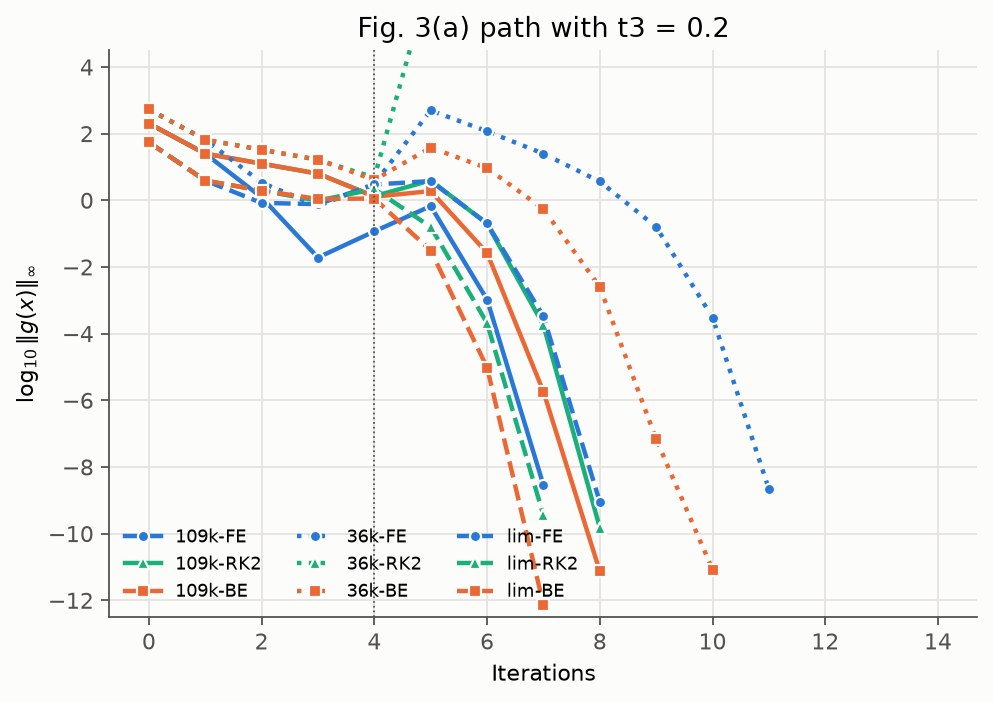
\includegraphics[width=\linewidth]{figures/repo/fig3a_pathway_t3_0.20.png}\caption{$t_3=0.20$}\end{subfigure}\hfill
\begin{subfigure}{0.325\textwidth}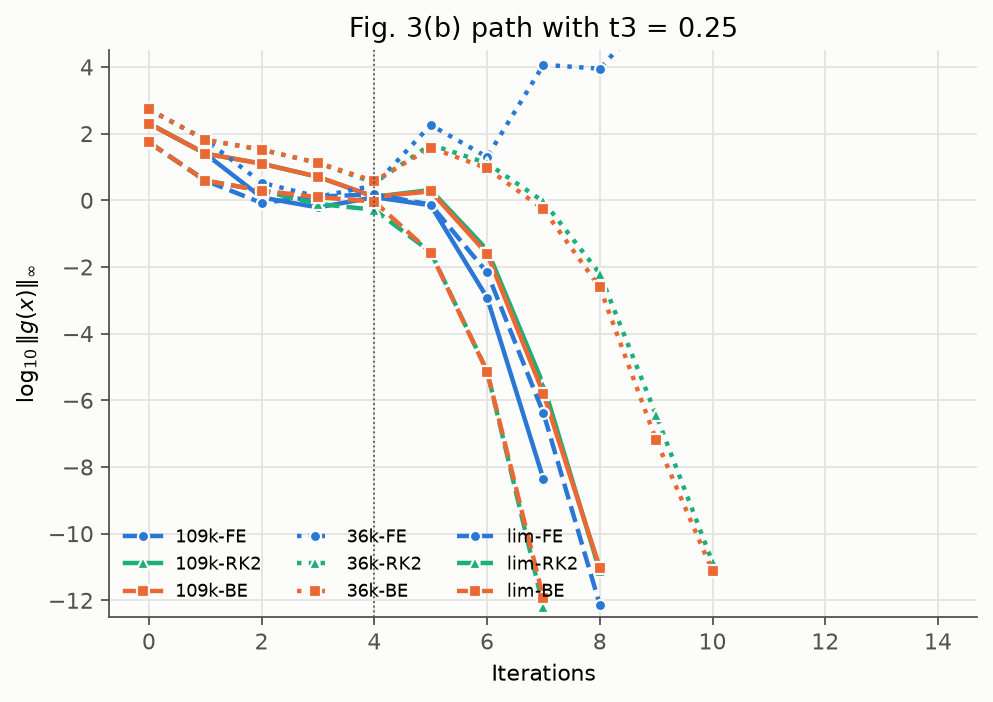
\includegraphics[width=\linewidth]{figures/repo/fig3b_pathway_t3_0.25.png}\caption{$t_3=0.25$}\end{subfigure}\hfill
\begin{subfigure}{0.325\textwidth}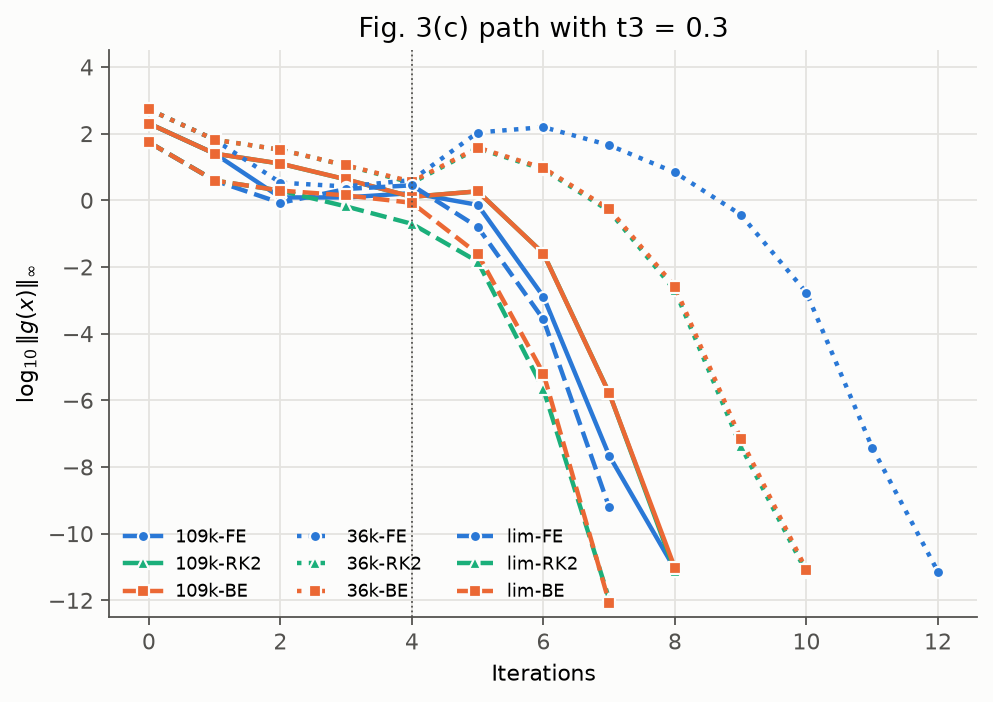
\includegraphics[width=\linewidth]{figures/repo/fig3c_pathway_t3_0.30.png}\caption{$t_3=0.30$}\end{subfigure}
\caption[Figure 3 re-run: five-point paths]{Figure 3 re-run: $\log_{10}\ninf{g}$ over the five homotopy
points (indices 0--4) and the NR iterations that follow, for \code{case109272} (solid), \code{case36964}
(dotted) and \code{case2000limit} (dashed).}
\label{fig:fig3}
\end{figure}

Table 6 times these runs (median of seven). On \code{case109272} our percentages of the NR-MAT time are
within 13 percentage points of the paper's in every row and within 8 in most (FE 143--164\% against
145--170\%, RK2 224--225\% against 226--237\%, BE 163--164\% against 169--171\%). On \code{case36964} they
are close for FE and 20--30 points higher for RK2 and BE. On \code{case2000limit} they are not: we measure
237--342\%, the paper 61--94\%. We cannot explain a hybrid run being \emph{faster} than NR-MAT there,
because it does strictly more work: four homotopy LUs plus three NR iterations, against NR-MAT's three
iterations. The full table is \cref{tab:t6} in the appendix.

\subsection{Figures 4 and 5: the states themselves}
The paper's Figure 4 follows five bus voltages of \code{case109272} through a two-point BE path and NR.
Ours (\cref{fig:fig4}) shows the same shape: angles overshoot to about 60 degrees at $t=1$ and NR pulls them
back within one iteration; bus 6 ends at \SI{1.0045}{pu} and 21.10 degrees. The mismatch goes
$201\to25\to1.26$ along the path and $1.70\to1.7\times10^{-2}\to7.3\times10^{-7}\to8.8\times10^{-12}$ in NR:
four NR iterations, as the paper reports.

\begin{figure}[!htbp]
\centering
\begin{minipage}[c]{0.44\textwidth}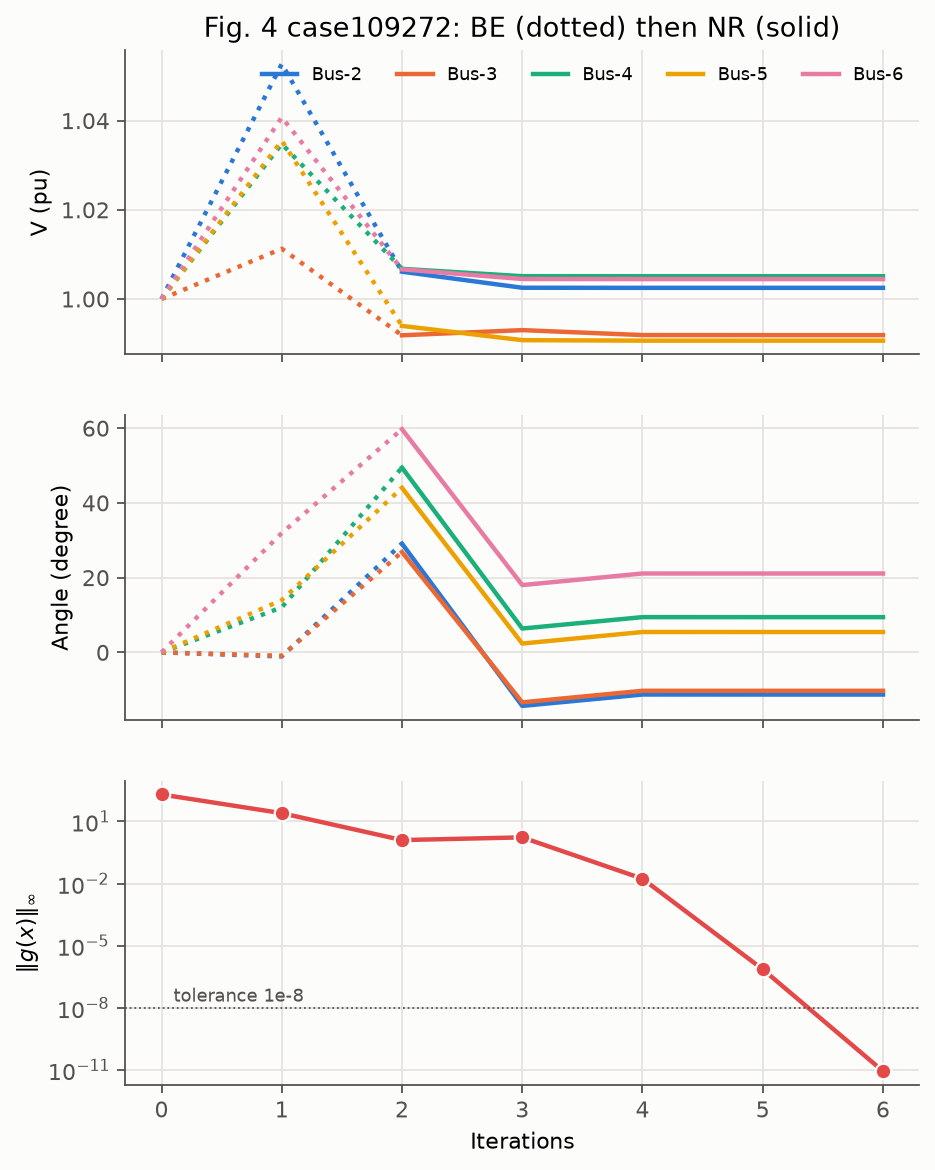
\includegraphics[width=\linewidth]{figures/repo/fig4_case109272_states.png}\end{minipage}\hfill
\begin{minipage}[c]{0.53\textwidth}
\caption[Figure 4 re-run: voltages of case109272]{Figure 4 re-run: voltage magnitudes and angles of buses
2--6 of \code{case109272} along the two-point BE path (dotted, points 0--2) and NR (solid). The paper draws
the mismatch on a second axis; we give it its own panel. The large angle excursion at $t=1$ is harmless:
the state is already inside NR's region of convergence.}
\label{fig:fig4}
\vspace{6pt}
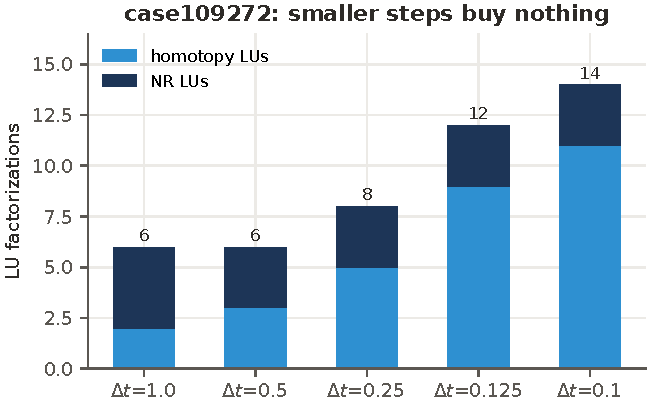
\includegraphics[width=\linewidth]{figures/fig5_tradeoff.pdf}
\captionof{figure}[Figure 5 re-run: the cost of smaller steps]{Figure 5 re-run in cost terms: LU factorizations
for each constant step $\Delta t$ after $t_1$. Every run ends at the same state (bus 6: \SI{1.0045}{pu},
21.10\textdegree).}
\label{fig:fig5}
\end{minipage}
\end{figure}

Figure 5 of the paper varies the constant step after $t_1$; \cref{fig:fig5full} is our version. Smaller
steps give NR a closer start (bus 6 at 28.2 degrees for $\Delta t=0.1$ against 59.7 for $\Delta t=1$) and
save one NR iteration, but each extra path point costs an LU, so total cost rises from 6 to 14
factorizations (\cref{fig:fig5}). This is the paper's own conclusion, now in numbers.

\begin{figure}[!htbp]
\centering
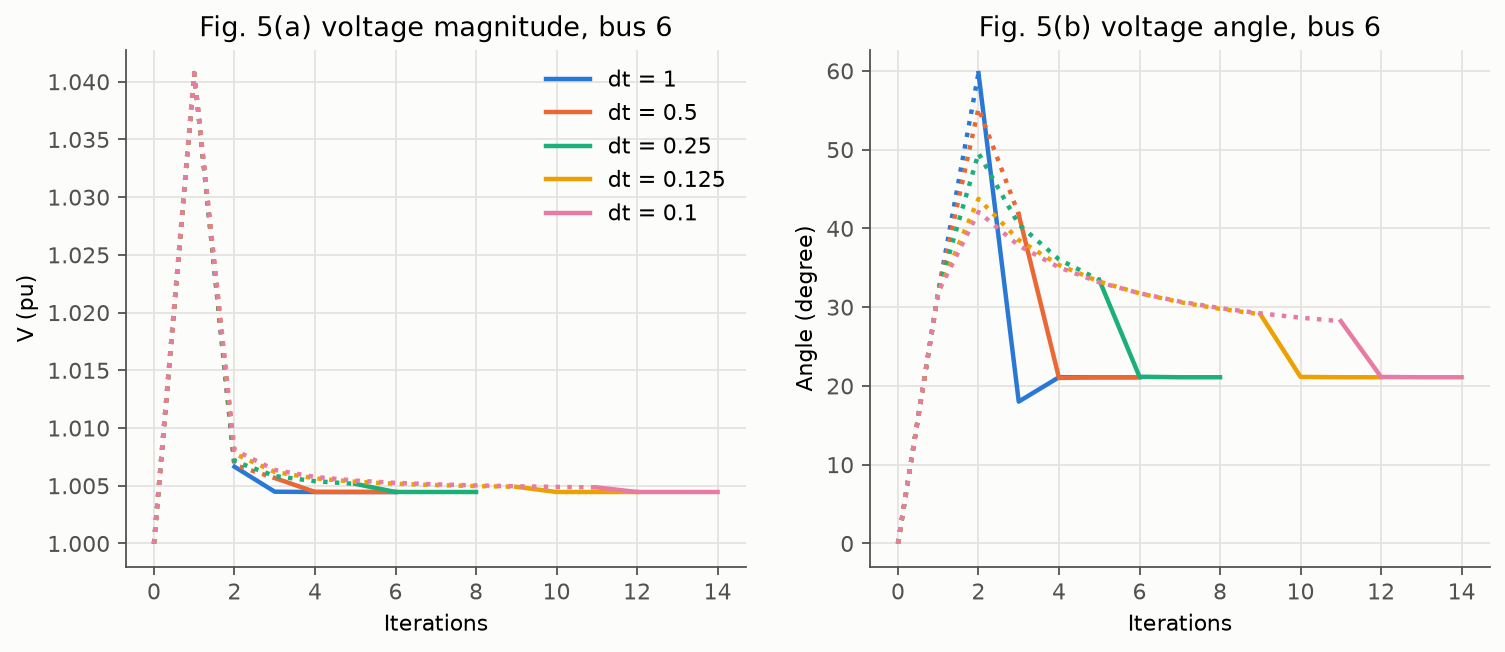
\includegraphics[width=\textwidth]{figures/repo/fig5_timestep_sensitivity.png}
\caption[Figure 5 re-run: bus 6 of case109272 for five time steps]{Figure 5 re-run: voltage magnitude (a)
and angle (b) of bus 6 of \code{case109272} for five constant steps $\Delta t$ after $t_1$; dotted is BE, solid
is NR. Whatever the step, every run ends at \SI{1.0045}{pu} and 21.10 degrees.}
\label{fig:fig5full}
\end{figure}

\subsection{Table 7: iterations}\label{sec:t7}
Table 7 is the paper's headline comparison. \Cref{tab:t7} gives ours. NR from the flat start fails on all
five ill-conditioned grids; BE(NR) needs 4 iterations and RK2(NR) 3 on all of them; FDXB counts match
to the iteration. 54 of the 63 cells agree exactly. Six of the nine differences are the two small limit
cases, whose NR-MAT, NR-flat and GSH-NR counts match the paper only on the stored 10\,MVA base
(\cref{tab:t7native}); the others are our GSH-NR reconstruction on two systems and one FDXB count for
\code{case109272}, discussed in \cref{sec:audit}. Every converged run in the table was also checked
against the reference operating point of \cref{sec:data}: all of them reach it, so none of these counts
is inflated by convergence to another root.

\begin{table}[!htbp]
\centering
\caption[Table 7 re-run: iterations of every method]{Table 7 re-run: iterations of the refining solver
(ours / paper). NR-MAT starts from the case file; all others from the flat start. BE uses the path
$\{0,0.005,1\}$, RK2 the seven-point path of the paper. Mismatches are in \textbf{bold}.}
\label{tab:t7}
\small
\setlength{\tabcolsep}{4.5pt}
\begin{tabular}{@{}l c c c c c c c@{}}
\toprule
\headrow \thead{Case} & \thead{NR-MAT} & \thead{NR-flat} & \thead{GSH-NR} & \thead{BE(NR)} & \thead{RK2(NR)} & \thead{BE(FDXB)} & \thead{RK2(FDXB)} \\
\midrule
\code{case18482}  & 6 / 6 & \fail\ / \fail & 10 / 10 & 4 / 4 & 3 / 3 & 33 / 33 & 29 / 29 \\
\code{case27318}  & 5 / 5 & \fail\ / \fail & \textbf{\fail\ / 25} & 4 / 4 & 3 / 3 & 29 / 29 & 25 / 25 \\
\code{case36964}  & 6 / 6 & \fail\ / \fail & \textbf{28 / 27} & 4 / 4 & 3 / 3 & 33 / 33 & 29 / 29 \\
\code{case54636}  & 5 / 5 & \fail\ / \fail & \fail\ / \fail & 4 / 4 & 3 / 3 & 29 / 29 & 25 / 25 \\
\code{case109272} & 5 / 5 & \fail\ / \fail & \fail\ / \fail & 4 / 4 & 3 / 3 & \textbf{29 / 19} & 25 / 25 \\
\code{case69limit}   & \textbf{2 / 4} & \textbf{2 / 4} & \textbf{2 / 4} & 1 / 1 & 1 / 1 & 8 / 8 & 8 / 8 \\
\code{case141limit}  & \textbf{2 / 3} & \textbf{2 / 3} & \textbf{2 / 3} & 1 / 1 & 1 / 1 & 8 / 8 & 6 / 6 \\
\code{case500limit}  & 3 / 3 & 4 / 4 & 4 / 4 & 2 / 2 & 2 / 2 & 13 / 13 & 11 / 11 \\
\code{case2000limit} & 3 / 3 & 5 / 5 & 5 / 5 & 3 / 3 & 3 / 3 & 22 / 22 & 20 / 20 \\
\bottomrule
\end{tabular}
\end{table}

\subsection{Table 8: run time}\label{sec:t8}
\Cref{fig:timing} is our Table 8, the median of seven runs relative to NR-MAT. BE(FDXB) is faster than
NR-MAT on all five ill-conditioned systems, at 66--93\% of its time against the paper's 57--85\%, and
BE(NR) costs slightly more than NR-MAT (102--122\% against 92--128\%). Both conclusions of the paper hold.
RK2 is much slower for us (252--331\% with either refiner) than for the paper (84--218\%): it needs seven
path points and two LUs per point, and in Python the per-LU overhead is not hidden. Our GSH-NR is also far
cheaper relative to NR-MAT than the paper's (176\% and 480\% against 1150\% and 2157\%), a reminder that it
is a reconstruction. Absolute times depend on the machine and on its load, which on a laptop is not under
our control; percentages of NR-MAT measured in the same session are more stable, and LU counts do not
depend on the machine at all. That is why the cost comparison of our own modifications uses LU counts.

\begin{figure}[!htbp]
\centering
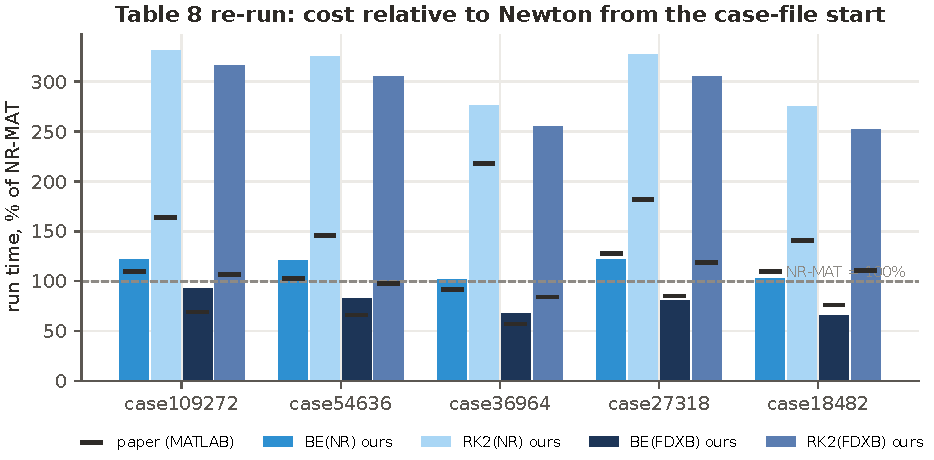
\includegraphics[width=0.95\textwidth]{figures/timing.pdf}
\caption[Table 8 re-run: run time relative to NR-MAT]{Table 8 re-run: median run time of seven repetitions
as a percentage of NR-MAT (bars) against the paper's MATLAB percentages (black ticks).}
\label{fig:timing}
\end{figure}

\begin{finding}[What the reproduction establishes.]
The method works as the paper says. On all five ill-conditioned grids, a two-point backward-Euler path
turns a divergent flat start into a four-iteration NR solve, and our numbers track the paper's across 28
orders of magnitude. Where explicit schemes fail, they fail where the paper says they do, and for the
reason \cref{sec:firststep} gives.
\end{finding}

% ============================================================================ 6 AUDIT
\section{Auditing the Base Paper}\label{sec:audit}

A reproduction is only useful if disagreements are chased down rather than averaged away. For every
difference we first checked our own code; the eight below survived that check. \Cref{tab:audit} lists them
with the evidence and what we did.

\begin{table}[!htbp]
\centering
\caption[Eight places where the paper is inconsistent or under-specified]{Eight places where the base paper
is inconsistent or under-specified, the evidence, and how our implementation handles each.}
\label{tab:audit}
\footnotesize
\begin{tabularx}{\textwidth}{@{}>{\raggedright\arraybackslash}p{3.2cm} L >{\raggedright\arraybackslash}p{3.1cm}@{}}
\toprule
\headrow \thead{Issue} & \thead{Evidence} & \thead{Our handling} \\
\midrule
Base MVA of \code{case69limit} and \code{case141limit} &
The files store 10\,MVA. Tables 2--5 match only on 100\,MVA; Table 7's NR-MAT/NR-flat counts (4, 3) match only on 10\,MVA, where BE(NR) then needs 2, not 1. No single base reproduces both. &
Use 100\,MVA; report the 10\,MVA counts separately (\cref{tab:t7native}). \\
\rowcolor{mist}
BE(FDXB) $=19$ for \code{case109272} (Table 7) &
We get 29, the same as \code{case54636}. The two systems are 8 and 4 copies of one network and are identical in every other cell of every table, the paper's included. &
Reported; most likely a typo. \\
Table 2, FE on \code{case18482} at $t=0.01$ &
Paper 9.7, ours 3.7; every other cell of that column matches to two digits. &
Reported, unresolved. \\
\rowcolor{mist}
Fig.~1(a), $\epsilon=0.05$ &
One NR step from $(1,0.95)$ gives $x=(6.01,-4.01)$ and $\ninf{g}\approx 99.5$, i.e.\ $\log_{10}\approx2$; the paper's curve starts near 3. We also need 8 iterations, not 9. &
Computed by hand and in code. \\
GSH-NR specification &
Described in words only; no formula for the shunts or for $\delta$. Our reconstruction matches \code{case18482} (10) and nearly \code{case36964} (28 vs 27) but fails on \code{case27318} (paper: 25). &
Our version documented in \code{gsh.py}. \\
\rowcolor{mist}
Section 4.4, $\Delta t_0=0.1$ &
``Does not work'' is stated without the path used. With $\{0,0.1,1\}$ BE works on 8 of 9 systems; with $\{0,0.1,0.2,0.3,1\}$ it fails on the four largest with NR. &
Both paths reported (\cref{fig:sec44}). \\
Table 6, RK2 with $t_3=0.20$ on \code{case36964} &
The paper reports success (232\%); in our run RK2 diverges on this path. &
Reported. \\
\rowcolor{mist}
Flat-start mismatch of \code{case2000limit} &
Tables 2--4 print 54, Table 5 prints 55 for the same starting point (ours: 54.95). &
Cosmetic; shows rounding. \\
\bottomrule
\end{tabularx}
\end{table}

Two conventions are not errors but had to be discovered before anything matched: FDXB iterations are
counted as $P$ updates plus $Q$ updates (not as MATPOWER's cycles), and the flat start includes the slack
angle. With those fixed, the base-MVA issue is the only one that changes a conclusion, and only for the
two smallest systems. The paper does not say whether its converged runs reach the intended operating
point; with its own settings all nine of its systems do in our runs (\cref{sec:rootcheck}), so this does
not affect any of its tables.

\begin{table}[h]
\centering
\caption[Table 7 on the stored 10 MVA base]{The two small limit cases on the base stored in the file (ours / paper).}
\label{tab:t7native}
\small
\begin{tabular}{@{}l c c c@{}}
\toprule
\headrow \thead{Case, 10 MVA base} & \thead{NR-MAT} & \thead{NR-flat} & \thead{BE(NR)} \\
\midrule
\code{case69limit}  & 4 / 4 & 4 / 4 & 2 / 1 \\
\code{case141limit} & 3 / 3 & 3 / 3 & 2 / 1 \\
\bottomrule
\end{tabular}
\end{table}

% ============================================================================ 7 MODIFICATIONS
\section{Our Modifications}\label{sec:mods}

\subsection{From proposal to implementation}
Our course proposal, a presentation given before any code was written, promised RK4 and Richardson-controlled steps for the path, a
spectral study of the flat-start Jacobian, maps of the feasible $(K,\Delta t_0)$ region, golden-section
tuning and linear solvers written from scratch. All of them are now in the repository
(\cref{fig:proposal}); the spectral, feasibility, tuning and linear-solver studies are reported in
\cref{sec:proposal}. Building the reproduction first also added items the proposal did not foresee: once
it was clear (\cref{sec:firststep}) that the method is a shifted Newton step followed by a near-Newton step,
the Newton stages themselves became the most promising place to intervene, which is where the optimal
multiplier and the corrector come from. One proposal item changed form: the Richardson estimate uses step
doubling rather than an embedded pair, so it works with any of the step rules.

\begin{figure}[!htbp]
\centering
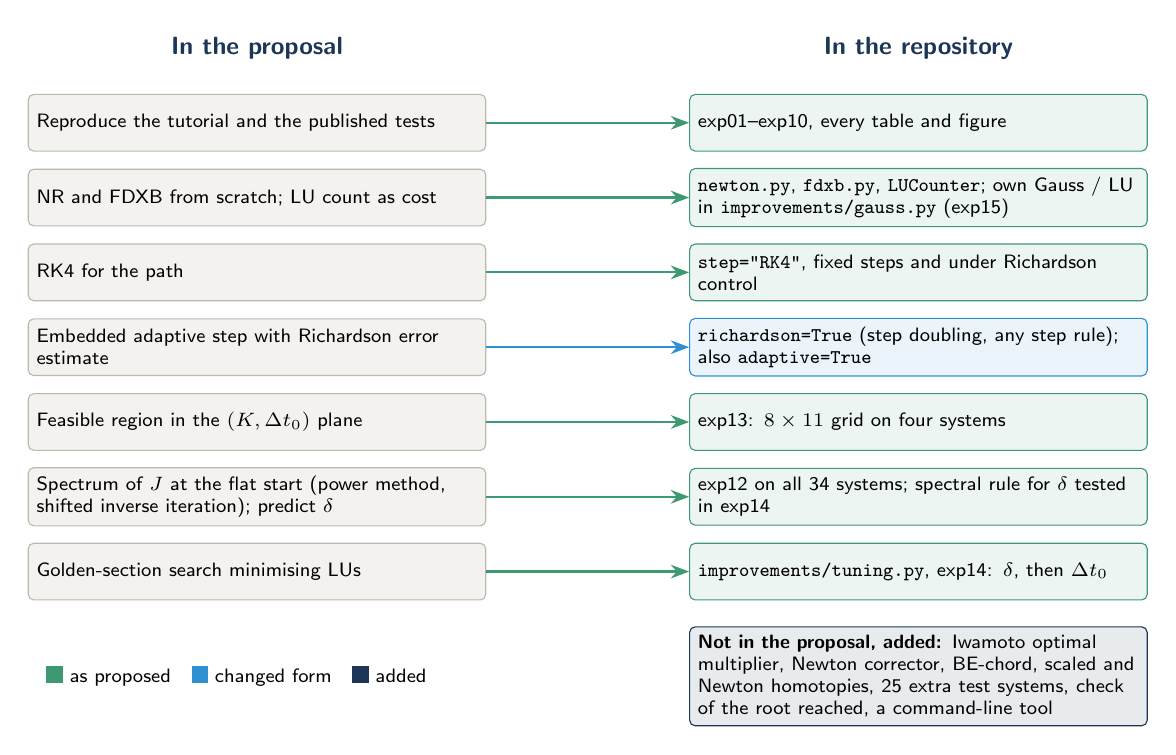
\begin{tikzpicture}[
  p/.style={draw=rulegrey,fill=mist,rounded corners=2pt,font=\sffamily\scriptsize,align=left,text width=5.6cm,inner sep=3pt,minimum height=0.72cm},
  b/.style={draw=#1,fill=#1!10,rounded corners=2pt,font=\sffamily\scriptsize,align=left,text width=5.6cm,inner sep=3pt,minimum height=0.72cm},
  lk/.style={-{Stealth},thick,draw=#1}, y=0.95cm]
  \node[font=\sffamily\small\bfseries,text=navy] at (0,1.0) {In the proposal};
  \node[font=\sffamily\small\bfseries,text=navy] at (8.4,1.0) {In the repository};
  \node[p] (p1) at (0,0)  {Reproduce the tutorial and the published tests};
  \node[p] (p2) at (0,-1) {NR and FDXB from scratch; LU count as cost};
  \node[p] (p3) at (0,-2) {RK4 for the path};
  \node[p] (p4) at (0,-3) {Embedded adaptive step with Richardson error estimate};
  \node[p] (p5) at (0,-4) {Feasible region in the $(K,\Delta t_0)$ plane};
  \node[p] (p6) at (0,-5) {Spectrum of $J$ at the flat start (power method, shifted inverse iteration); predict $\delta$};
  \node[p] (p7) at (0,-6) {Golden-section search minimising LUs};
  \node[b=sage] (b1) at (8.4,0)  {exp01--exp10, every table and figure};
  \node[b=sage] (b2) at (8.4,-1) {\code{newton.py}, \code{fdxb.py}, \code{LUCounter}; own Gauss / LU in \code{improvements/gauss.py} (exp15)};
  \node[b=sage] (b3) at (8.4,-2) {\code{step="RK4"}, fixed steps and under Richardson control};
  \node[b=skyblue] (b4) at (8.4,-3) {\code{richardson=True} (step doubling, any step rule); also \code{adaptive=True}};
  \node[b=sage] (b5) at (8.4,-4) {exp13: $8\times11$ grid on four systems};
  \node[b=sage] (b6) at (8.4,-5) {exp12 on all 34 systems; spectral rule for $\delta$ tested in exp14};
  \node[b=sage] (b7) at (8.4,-6) {\code{improvements/tuning.py}, exp14: $\delta$, then $\Delta t_0$};
  \foreach \i/\c in {1/sage,2/sage,3/sage,4/skyblue,5/sage,6/sage,7/sage} \draw[lk=\c] (p\i.east) -- (b\i.west);
  \node[b=navy,text width=5.6cm] (x1) at (8.4,-7.4) {\textbf{Not in the proposal, added:} Iwamoto optimal multiplier, Newton corrector, BE-chord, scaled and Newton homotopies, 25 extra test systems, check of the root reached, a command-line tool};
  \node[font=\sffamily\scriptsize,anchor=west] at (-2.8,-7.4) {\textcolor{sage}{\rule{6pt}{6pt}} as proposed\quad \textcolor{skyblue}{\rule{6pt}{6pt}} changed form\quad \textcolor{navy}{\rule{6pt}{6pt}} added};
\end{tikzpicture}
\caption[From proposal to implementation]{What the proposal promised and what the repository contains.}
\label{fig:proposal}
\end{figure}

\subsection{Design rule: switches on top of an untouched reproduction}
Every modification is a field of one immutable \code{Options} object in \code{improvements/solve.py}. All
fields default to the paper's method, the reproduced \code{dynhomotopy} package is imported but never
edited, and a test checks that \code{Options()} reproduces the paper's result exactly. This makes each
comparison a controlled experiment: exactly one thing differs.

\begin{codebox}{Listing 2 \quad Using a modification, from Python and from the command line}
\begin{lstlisting}[style=py,numbers=none]
from improvements import Options, solve
result = solve(pf, pf.flat_start(), K=1e-4, times=[0, 0.005, 1],
               options=Options(multiplier=True, corrector=True))
\end{lstlisting}
\vspace{-4pt}
\begin{lstlisting}[language=bash,basicstyle=\ttfamily\footnotesize,numbers=none,columns=fullflexible]
python -m improvements case36964 --corrector --multiplier      # printed next to the paper's method
python -m improvements case6024 --richardson --dt0 0.05 --K 1e-3
\end{lstlisting}
\end{codebox}

\Cref{fig:switches} shows where each switch acts in the pipeline. The next subsections define them.
\code{adaptive} and \code{richardson} both choose the time points, so they cannot be combined.

\begin{figure}[!htbp]
\centering
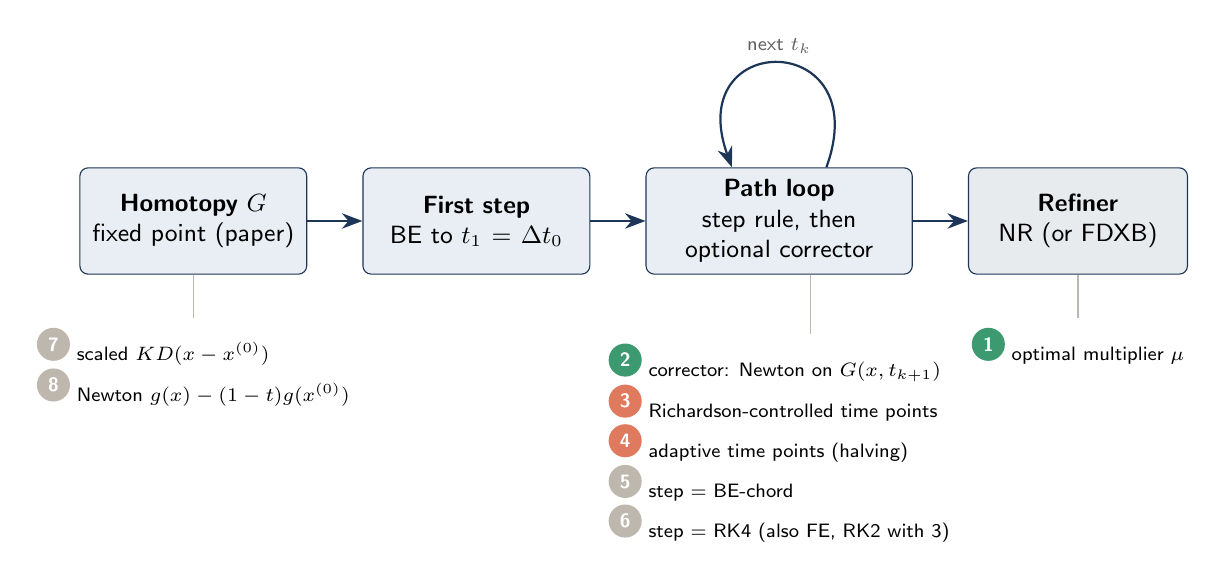
\begin{tikzpicture}[node distance=0.7cm]
  \node[stage=2.6cm] (g) {\textbf{Homotopy $G$}\\ fixed point (paper)};
  \node[stage=2.6cm,right=of g] (f) {\textbf{First step}\\ BE to $t_1=\Delta t_0$};
  \node[stage=3.1cm,right=of f] (l) {\textbf{Path loop}\\ step rule, then\\ optional corrector};
  \node[stage=2.5cm,right=of l,fill=navy!10,draw=navy] (r) {\textbf{Refiner}\\ NR (or FDXB)};
  \draw[flow] (g) -- (f); \draw[flow] (f) -- (l); \draw[flow] (l) -- (r);
  \draw[flow] ([xshift=6mm]l.north) to[out=70,in=110,looseness=4] node[above,note]{next $t_k$} ([xshift=-6mm]l.north);
  % tags
  \node[font=\sffamily\scriptsize,align=left,anchor=north] (tg) at ([yshift=-0.55cm]g.south) {\tikz\node[xbadge]{7}; scaled $K D(x-\xo)$\\ \tikz\node[xbadge]{8}; Newton $g(x)-(1-t)g(\xo)$};
  \node[font=\sffamily\scriptsize,align=left,anchor=north] (tl) at ([yshift=-0.75cm]l.south) {\tikz\node[gbadge]{2}; corrector: Newton on $G(x,t_{k+1})$\\ \tikz\node[badge,fill=coral]{3}; Richardson-controlled time points\\ \tikz\node[badge,fill=coral]{4}; adaptive time points (halving)\\ \tikz\node[xbadge]{5}; step = BE-chord\\ \tikz\node[xbadge]{6}; step = RK4 (also FE, RK2 with 3)};
  \node[font=\sffamily\scriptsize,align=left,anchor=north] (tr) at ([yshift=-0.55cm]r.south) {\tikz\node[gbadge]{1}; optimal multiplier $\mu$};
  \draw[rulegrey] (g.south) -- (tg.north); \draw[rulegrey] (l.south) ++(0.4,0) -- ([xshift=0.4cm]tl.north); \draw[rulegrey] (r.south) -- (tr.north);
\end{tikzpicture}
\caption[Where each of the eight switches acts]{Where each of the eight switches acts. Green badges: the two
that help on their own and together (\cref{sec:modresults}); orange: the two path-control rules, which help
on some systems at a price; grey: the four that did not work.}
\label{fig:switches}
\end{figure}

\subsection{Modification 1: the optimal multiplier in NR}
After the homotopy, the state is inside NR's region of convergence but not deep inside it; the first NR
steps can still overshoot (the angles in \cref{fig:fig4} jump by 40 degrees). Iwamoto and
Tamura~\cite{iwamoto1981} scale each Newton step $\Delta x$ by a factor $\mu$. With $a=g(x)$ and
$c=g(x+\Delta x)$, the mismatch along the step is modelled as
\begin{equation}
  g(x+\mu\,\Delta x) \approx (1-\mu)\,a + \mu^2 c,
\end{equation}
which is exact when $g$ is quadratic (power flow in rectangular coordinates) and a good model in polar
coordinates. Minimising $\norm{(1-\mu)a+\mu^2c}_2^2$ and setting the derivative to zero gives the cubic
\begin{keyeq}
\begin{equation}
  2(c^{\top}c)\,\mu^3 - 3(a^{\top}c)\,\mu^2 + (a^{\top}a + 2a^{\top}c)\,\mu - a^{\top}a = 0,
\end{equation}
\end{keyeq}
and we take the real root in $(0,2]$ with the smallest model mismatch. NR evaluates $g(x+\Delta x)$
anyway, so the multiplier costs one extra mismatch evaluation when $\mu\neq1$ and no extra LU. Near the
solution $c\to0$ and $\mu\to1$, so quadratic convergence is kept.

\begin{algo}{Algorithm 2 \quad NR with the optimal multiplier (\texttt{improvements/multiplier.py})}
\begin{algorithmic}[1]
\Require $x$, tolerance $10^{-8}$, at most 10 iterations
\While{$\ninf{g(x)}\ge 10^{-8}$ \textbf{and} fewer than 10 iterations}
  \State $\Delta x \gets -J(x)^{-1}g(x)$ \Comment{one LU}
  \State $a\gets g(x)$,\ \ $c\gets g(x+\Delta x)$
  \State $\mu \gets$ best real root in $(0,2]$ of the cubic, or 1 if none
  \State $x\gets x+\mu\,\Delta x$
\EndWhile
\end{algorithmic}
\end{algo}

\subsection{Modification 2: a Newton corrector after every step}
Predictor--corrector continuation~\cite{allgower2003} follows every predictor step with a Newton step back
onto the path. Here, after any step to $t_{k+1}$ we take one Newton step on $G(x,t_{k+1})=0$:
\begin{equation}
  x_{k+1} \gets x_{k+1} - G_x(x_{k+1},t_{k+1})^{-1}\,G(x_{k+1},t_{k+1}),
\end{equation}
at the cost of one extra LU per path point. On the first step this is again a shifted-Jacobian step; at
$t=1$ it is, exactly, one NR step on $g$, a fact that matters for how its results are read
(\cref{sec:pc-accounting}).

\subsection{Modification 3: Richardson error control of the path steps}\label{sec:richardson}
The paper chooses its path points by hand; our proposal asked for steps chosen by an error estimate. After
the paper's BE step to $t_1=\Delta t_0$, each attempt from $t$ with step $\Delta t$ computes one step of
size $\Delta t$, $x_{\mathrm{full}}$, and two steps of size $\Delta t/2$, $x_{\mathrm{half}}$. For a rule of
order $p$ their difference estimates the error of the half steps,
\begin{keyeq}
\begin{gather}
  \varepsilon = \frac{\ninf{x_{\mathrm{half}}-x_{\mathrm{full}}}}{2^p-1}, \qquad
  x_{\mathrm{new}} = x_{\mathrm{half}} + \frac{x_{\mathrm{half}}-x_{\mathrm{full}}}{2^p-1}, \\
  \Delta t \gets \Delta t\cdot\min\!\Bigl(4,\ \max\bigl(0.1,\ 0.9\,(\mathrm{tol}/\varepsilon)^{1/(p+1)}\bigr)\Bigr).
\end{gather}
\end{keyeq}
The step is kept if $\varepsilon\le\mathrm{tol}=0.5$ (radians and per unit), and then the kept point is
the Richardson extrapolation $x_{\mathrm{new}}$; either way the next $\Delta t$ is scaled as shown. A step
that breaks down (singular matrix or non-finite mismatch) is retried at a quarter of its size. Every
attempt costs three steps, so with BE three LUs, and a path that needs more than 150 LUs is stopped and
counted as a failure. The step rule is a switch: BE ($p=1$, the paper's rule), FE ($p=1$), RK2 ($p=2$) or
RK4 ($p=4$), always after a BE first step. The large tolerance is deliberate: the path only has to end
inside NR's region of convergence, not on the exact homotopy curve.

\begin{algo}{Algorithm 3 \quad Richardson-controlled path (\texttt{improvements/path.py})}
\begin{algorithmic}[1]
\State $x\gets\textsc{BE}(\xo,0,\Delta t_0)$;\quad $t\gets\Delta t_0$;\quad $\Delta t\gets 1-\Delta t_0$
\While{$t<1$ \textbf{and} at most 150 LUs used}
  \State $\Delta t\gets\min(\Delta t,1-t)$;\quad $x_f\gets\textsc{Step}(x,t,\Delta t)$;\quad
         $x_h\gets\textsc{Step}(\textsc{Step}(x,t,\tfrac{\Delta t}{2}),t+\tfrac{\Delta t}{2},\tfrac{\Delta t}{2})$
  \State \textbf{if} a step broke down \textbf{then} $\Delta t\gets\Delta t/4$ and \textbf{continue}
  \State $\varepsilon\gets\ninf{x_h-x_f}/(2^p-1)$
  \If{$\varepsilon\le\mathrm{tol}$} \State $x\gets x_h+(x_h-x_f)/(2^p-1)$;\quad $t\gets t+\Delta t$ \EndIf
  \State $\Delta t\gets\Delta t\cdot\min(4,\max(0.1,\,0.9(\mathrm{tol}/\varepsilon)^{1/(p+1)}))$
\EndWhile
\end{algorithmic}
\end{algo}

\subsection{Modification 4: choosing the time points by the mismatch}
A cheaper rule controls the step by the quantity NR cares about. It keeps the paper's first step to
$t_1=\Delta t_0$, then tries to jump straight to $t=1$; a step is kept if it reduced $\ninf{g}$, otherwise
it is halved (at most six times); after an accepted step the next one is doubled. Rejected trials still
count as LUs. \Cref{sec:adaptive-fail} shows the price of using $\ninf{g}$ as the test.

\begin{algo}{Algorithm 4 \quad Adaptive path (\texttt{improvements/path.py})}
\begin{algorithmic}[1]
\State $x\gets\textsc{BE}(\xo,0,\Delta t_0)$;\quad $t\gets\Delta t_0$;\quad $\Delta t\gets 1-\Delta t_0$
\While{$t<1$}
  \For{up to 7 trials}
    \State $\Delta t\gets\min(\Delta t,1-t)$;\quad $\tilde x\gets\textsc{Step}(x,t,\Delta t)$ \Comment{one LU per trial}
    \If{$\ninf{g(\tilde x)}<\ninf{g(x)}$} \textbf{break} \Else\ $\Delta t\gets\Delta t/2$ \EndIf
  \EndFor
  \State \textbf{if} no trial was accepted \textbf{then return} failure
  \State $x\gets\tilde x$;\quad $t\gets t+\Delta t$;\quad $\Delta t\gets 2\Delta t$
\EndWhile
\end{algorithmic}
\end{algo}

\subsection{Modifications 5--8: four ideas that did not work}
\begin{description}[font=\sffamily\bfseries\color{navy},leftmargin=0pt,itemsep=3pt]
  \item[5. BE-chord.] The paper remarks after its eq.~(19) that the single fixed-point iteration of BE
        could be refined. We do three iterations $\hat x\gets x_k-\Delta t\,G_x(x_k,t_{k+1})^{-1}G_t(\hat x)$,
        reusing one LU.
  \item[6. RK4 with fixed steps.] Classical fourth-order Runge--Kutta for the steps after $t_1$ (the
        paper's future work; also in our proposal). Under Richardson control it is modification 3 with
        $p=4$.
  \item[7. Scaled homotopy.] $g_0(x)=K D(x-\xo)$ with $D=|\mathrm{diag}\,J(\xo)|$ normalised to mean 1, so each
        equation is shifted in proportion to its own diagonal, in the spirit of~\cite{freitas2023}.
  \item[8. Newton homotopy.] The textbook $G(x,t)=g(x)-(1-t)g(\xo)$~\cite{watson1989}, for which
        $G_x=J(x)$ and there is no $KI$ term at all.
\end{description}

\subsection{Evaluation protocol}
The paper tunes its parameters on nine systems. To see whether a modification helps in general, we ran
every configuration on all 34 systems under five settings of $(\Delta t_0,K)$, all with the path
$\{0,\Delta t_0,1\}$ (\cref{fig:protocol}). The multiplier, corrector and adaptive switches were run in
all eight on/off combinations; Richardson control with each of BE, FE, RK2 and RK4 and together with the
multiplier; and the four other ideas alone. That gives 17 configurations and 2{,}890 runs. Each
configuration is run once, so run times are not compared; cost is the number of LU factorizations.

\begin{figure}[!htbp]
\centering
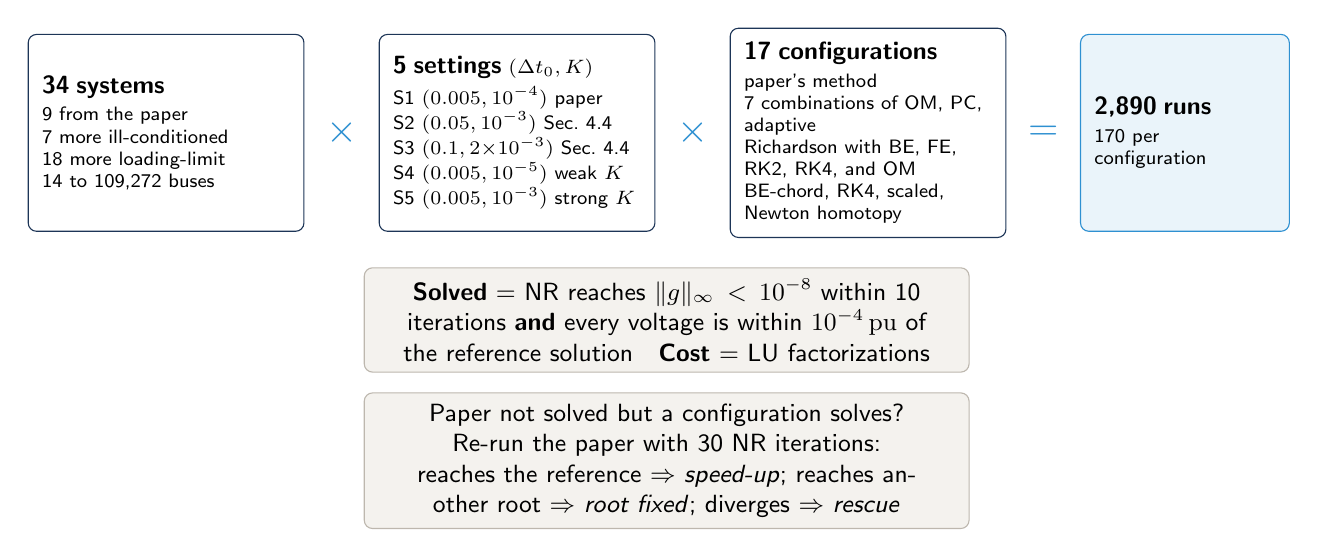
\begin{tikzpicture}[
  card/.style={draw=navy,fill=white,rounded corners=3pt,font=\sffamily\scriptsize,align=left,text width=3.15cm,inner sep=5pt,minimum height=2.5cm},
  op/.style={font=\sffamily\bfseries\Large,text=skyblue}]
  \node[card] (c1) {\textbf{\small 34 systems}\\[2pt] 9 from the paper\\ 7 more ill-conditioned\\ 18 more loading-limit\\ 14 to 109{,}272 buses};
  \node[op,right=0.15cm of c1] (m1) {$\times$};
  \node[card,right=0.15cm of m1] (c2) {\textbf{\small 5 settings} $(\Delta t_0,K)$\\[2pt] S1 $(0.005,10^{-4})$ paper\\ S2 $(0.05,10^{-3})$ Sec.\ 4.4\\ S3 $(0.1,2{\times}10^{-3})$ Sec.\ 4.4\\ S4 $(0.005,10^{-5})$ weak $K$\\ S5 $(0.005,10^{-3})$ strong $K$};
  \node[op,right=0.15cm of c2] (m2) {$\times$};
  \node[card,right=0.15cm of m2] (c3) {\textbf{\small 17 configurations}\\[2pt] paper's method\\ 7 combinations of OM, PC, adaptive\\ Richardson with BE, FE, RK2, RK4, and OM\\ BE-chord, RK4, scaled, Newton homotopy};
  \node[op,right=0.15cm of c3] (m3) {$=$};
  \node[card,right=0.15cm of m3,text width=2.3cm,fill=skyblue!10,draw=skyblue] (c4) {\textbf{\small 2{,}890 runs}\\[2pt] 170 per\\ configuration};
  \node[soft,below=0.45cm of c2,text width=7.4cm,xshift=1.9cm] (crit) {\textbf{Solved} = NR reaches $\ninf{g}<10^{-8}$ within 10 iterations \textbf{and} every voltage is within \SI{e-4}{pu} of the reference solution\quad \textbf{Cost} = LU factorizations};
  \node[soft,below=0.25cm of crit,text width=7.4cm] (re) {Paper not solved but a configuration solves? Re-run the paper with 30 NR iterations: reaches the reference $\Rightarrow$ \emph{speed-up}; reaches another root $\Rightarrow$ \emph{root fixed}; diverges $\Rightarrow$ \emph{rescue}};
\end{tikzpicture}
\caption[Evaluation protocol for the modifications]{Evaluation protocol for the modifications.}
\label{fig:protocol}
\end{figure}

% ============================================================================ 8 MOD RESULTS
\section{Results of the Modifications}\label{sec:modresults}

\subsection{First, which root? The paper's method on the wider test bed}\label{sec:rootcheck}
On the 170 runs of the test bed, the paper's method gives NR a start from which it converges within ten
iterations 141 times. But 14 of those 141 runs converge to a \emph{different} solution of the power flow
equations than the reference operating point of \cref{sec:data}: \code{case54636} and \code{case109272}
with the larger first step of S3 and with the weak or strong $K$ of S4 and S5, \code{case27318} in S4 and S5,
\code{case3012wplimit} and \code{case3375wplimit} already in the paper's own setting S1, and
\code{case13659pegaselimit} in S4. The mismatch is below $10^{-8}$ in every one of them, so a
convergence test alone cannot tell them apart; only comparing the voltages can. With the paper's own
settings all nine of the paper's systems reach the reference, so its published tables are not affected.
What is affected is how well the method transfers: it truly solves 127 of 170 runs, not 141. Every number
below counts a run as solved only if it reaches the reference, and counts the other-root runs separately.

\subsection{Headline numbers}
\Cref{tab:improve} and \cref{fig:solved} give the result of all 2{,}890 runs. Every configuration that
contains the corrector solves 152 and loses nothing; the multiplier alone solves 143; Richardson control
solves 145--158 depending on the step rule, at a much higher cost for the explicit rules. The four other
ideas lose runs, fixed-step RK4 catastrophically.

\begin{table}[!htbp]
\centering
\caption[Runs solved by each configuration]{Runs that reach the reference solution (of 34 per setting,
170 in total). \emph{Other}: runs that converge to a different root. \emph{Gained} and \emph{lost} are
relative to the paper's method, with gained split into (rescues / root fixed / speed-ups,
\cref{sec:rescue}). \emph{LUs S1}: mean factorizations in setting S1 on the systems both this configuration
and the paper's method solve (the paper's own mean on those systems in grey where it is not 8.04).
\emph{Ratio}: the same, all five settings pooled, relative to the paper's method.}
\label{tab:improve}
\footnotesize
\setlength{\tabcolsep}{3.1pt}
\begin{tabular}{@{}l r r r r r r r l r l r@{}}
\toprule
\headrow \thead{Configuration} & \thead{S1} & \thead{S2} & \thead{S3} & \thead{S4} & \thead{S5} & \thead{Total} & \thead{Other} & \thead{Gained} & \thead{Lost} & \thead{LUs S1} & \thead{Ratio} \\
\midrule
\rows{generated/improve_table.tex}
\bottomrule
\end{tabular}
\end{table}

\begin{figure}[!htbp]
\centering
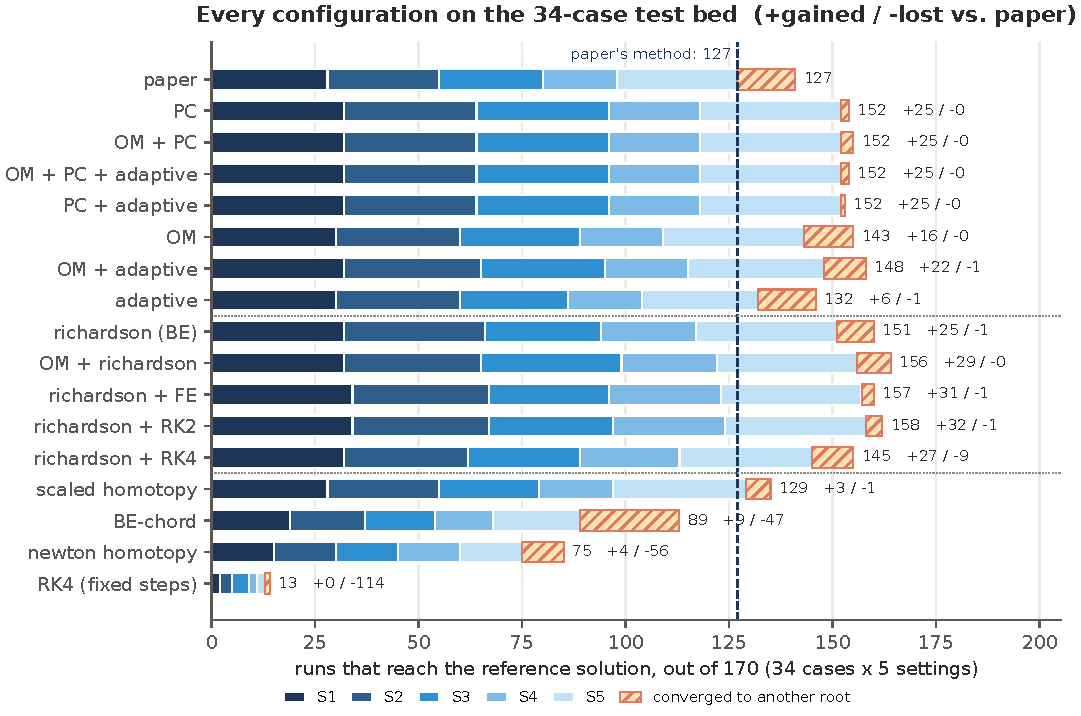
\includegraphics[width=\textwidth]{figures/improve_solved.pdf}
\caption[Runs solved per configuration, by setting]{Runs that reach the reference solution per
configuration, stacked by setting; the hatched segment is the runs that converge to another root. The
dashed line is the paper's method. Dotted lines separate the corrector/multiplier/adaptive family,
Richardson control and the four ideas that did not work.}
\label{fig:solved}
\end{figure}

\begin{finding}[The corrector is the robust improvement, the multiplier the cheap one.]
The Newton corrector alone solves 25 more runs than the paper's method (2 rescues, 13 wrong roots
corrected, 10 speed-ups), never loses one, and cuts the other-root runs from 14 to 2, for 0.4 more LUs per
system in S1 (8.43 against 8.04). It also makes the outcome almost independent of $\Delta t_0$: 32 of 34
systems in each of S1, S2 and S3. The optimal multiplier alone is 11\% cheaper (7.14 LUs) but still lands
on another root 12 times. Together, \textbf{multiplier plus corrector} keeps all of the corrector's
robustness (152 solved, no losses, 3 other-root runs) and most of the multiplier's saving (7.57 LUs in S1,
7\% fewer than the paper's method over all settings). It is the configuration we recommend.
\end{finding}

\subsection{Robustness against cost}
\Cref{fig:pareto} plots each configuration's solved count against its relative LU cost. Multiplier plus
corrector sits alone in the upper left: more robust \emph{and} cheaper than the paper's method. The
corrector alone is as robust but costs about 5\% more, because it adds one LU per path point. Combining the
corrector with adaptive steps is expensive (ratio 1.25--1.35): every rejected trial now costs two LUs, and in
setting S5 this averages about 20 LUs per run. Richardson control lies to the right: 18--30\% more LUs with
BE, and 4--8 times the paper's cost with FE, RK2 and RK4.

\begin{figure}[!htbp]
\centering
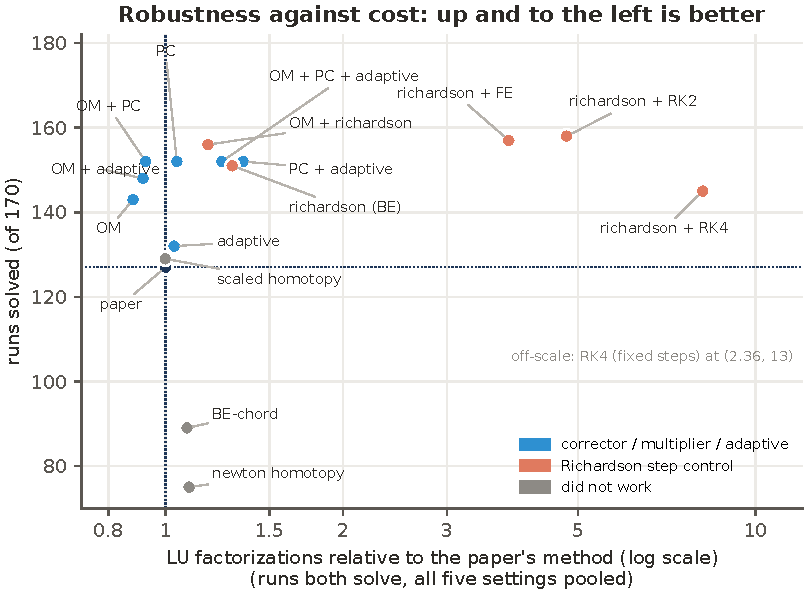
\includegraphics[width=0.78\textwidth]{figures/improve_pareto.pdf}
\caption[Robustness against cost]{Runs solved against LU cost relative to the paper's method (log scale).
Blue: the corrector, multiplier and adaptive switches and their combinations; orange: Richardson step
control with each step rule; grey: the four ideas that did not work.}
\label{fig:pareto}
\end{figure}

\subsection{Richardson step control}
Error-controlled steps are the only change that solves some runs nothing else solves. \code{case6024} in
the paper's own setting S1 is solved only by Richardson control (73 LUs with BE, with or without the
multiplier; 106 with FE, 112 with RK2), and \code{case7092}, \code{case10595} and \code{case12110} with the
weak $K$ of S4, where the paper's method diverges, are solved only by Richardson configurations. Multiplier
plus Richardson rescues 10 of the 11 divergent runs of the test bed---more than any other configuration---and
solves 156 runs without losing one.

\Cref{fig:richardson} shows what the controller does on \code{case6024}. The paper's jump from $t_1$ to
$t=1$ lands at a mismatch NR cannot recover from. The error estimate forces small steps over the early part of
the path, where the state changes fastest, and then lets them grow by up to four times per step; the path
ends much closer to the solution. The price is visible too: every attempt costs three steps, and rejected
attempts are paid for.

\begin{figure}[!htbp]
\centering
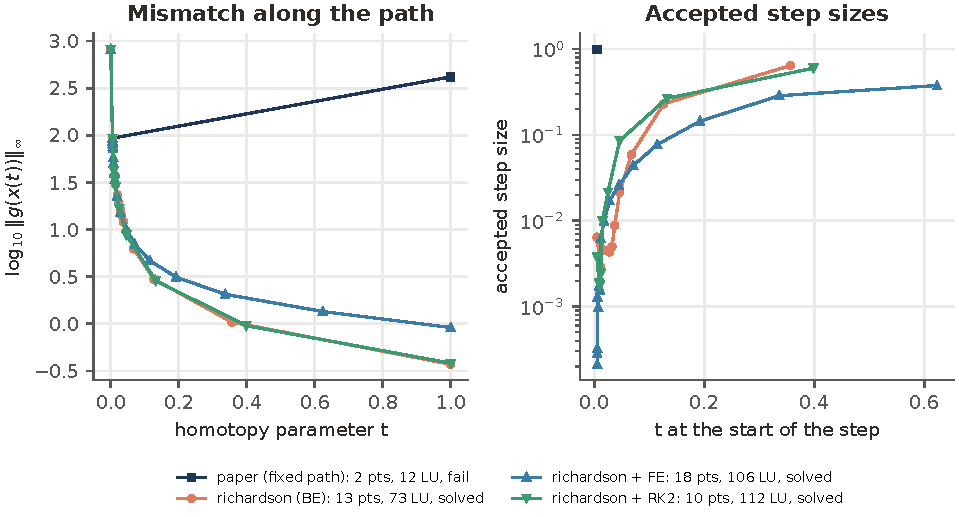
\includegraphics[width=\textwidth]{figures/richardson_path.pdf}
\caption[Richardson-controlled paths on case6024]{Richardson-controlled paths on \code{case6024}, setting
S1, the one system in S1 that only Richardson control solves. Left: mismatch at each accepted point (the
legend gives the points, the LUs including rejected attempts, and the outcome after NR). Right: the
accepted step sizes.}
\label{fig:richardson}
\end{figure}

The same study tests the paper's claim that BE is the right integrator, this time under error control
rather than with hand-picked steps. It holds: in S1, Richardson control needs 10.6 LUs with BE, 37 with FE,
48 with RK2 and 87 with RK4. FE and RK2 solve slightly more runs (157 and 158, against 151 for BE)---the
extra runs are almost all corrected wrong roots---but at four to six times the cost; RK4 solves fewer (145) and loses nine runs
the paper's method solves. Higher order does not pay here because the steps are limited by stability, not by
accuracy (\cref{sec:failure}). Richardson with BE still lands on another root 9 times; the corrector is much
better at that (2).

\subsection{System by system}
\Cref{fig:cases} shows the LU count of every configuration on every system in the paper's own setting S1.
On the paper's nine systems nothing much changes: the method already works there with 3--6 LUs, the
multiplier saves one LU on \code{case18482} and the corrector adds one on the limit cases. The differences
are on the added systems. Of the 14 extra limit cases that both the multiplier and the paper's method solve,
the multiplier saves one to three LUs on 13. On \code{case3012wplimit} and \code{case3375wplimit} the
paper's method and the multiplier both converge to another root; every configuration with the corrector
reaches the reference, with 9--11 LUs. Among the added ill-conditioned systems, \code{case6748} is solved
only by adaptive steps (18--19 LUs) and by Richardson control (49 LUs or more), and \code{case6024} only by
Richardson control.

\begin{figure}[p]
\centering
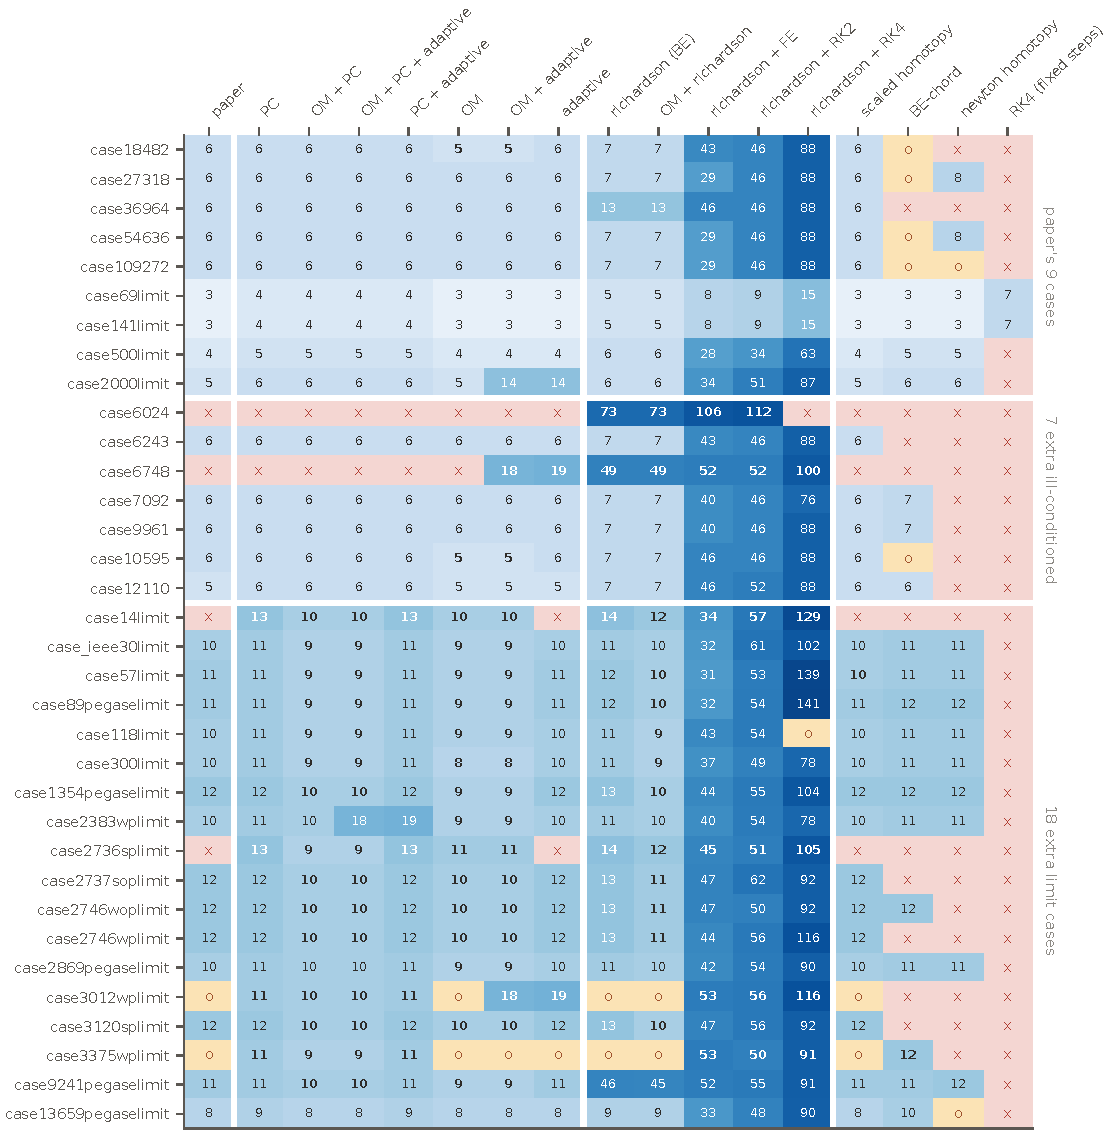
\includegraphics[width=\textwidth]{figures/improve_cases_s1.pdf}
\caption[LU factorizations per system and configuration, setting S1]{LU factorizations per system and
configuration in setting S1 (the paper's parameters). \textcolor{failred}{x}: fails; o: converges to
another root. Bold numbers are cheaper than the paper's method or solve a system it does not. White lines
separate the paper's systems, the extra ill-conditioned systems and the extra limit cases, and the
configuration families.}
\label{fig:cases}
\end{figure}

\subsection{Rescues, root fixes and speed-ups}\label{sec:rescue}
Because many limit cases sit exactly on NR's 10-iteration budget (\cref{sec:data}), a configuration can
``solve'' a system just by saving one iteration. We therefore re-ran the paper's method with 30 NR
iterations on every run it does not solve that some configuration does. There are 36 such runs, and they
are of three kinds:
\begin{itemize}
  \item \textbf{10 speed-ups.} \code{case14limit} and \code{case2736splimit} in every setting: the paper's
        method reaches the reference in 11 NR iterations, one more than allowed.
  \item \textbf{15 root fixes.} The paper's method converges, but to another root (\cref{sec:rootcheck}).
        The corrector fixes 13 of them; the other two (\code{case109272} and \code{case13659pegaselimit}
        in S4) only Richardson control with an explicit step rule fixes.
  \item \textbf{11 rescues.} The paper's method diverges even with 30 iterations: \code{case36964} in S2
        and S3, \code{case6024} in S1--S3, \code{case6748} in S1--S3, and \code{case7092},
        \code{case10595} and \code{case12110} in S4. Multiplier plus Richardson rescues 10 of them,
        Richardson with BE 9, multiplier plus adaptive 4, the corrector 2 and the multiplier 1.
\end{itemize}
The remaining 7 runs the paper's method does not solve are solved by nothing (\cref{sec:nothing}).

\Cref{fig:rescues} shows one run of each kind in full. On \code{case36964} in S2 the paper's NR wanders and
diverges; the multiplier converges in six iterations and the corrector in two. On \code{case3012wplimit}
the paper's method and the multiplier converge, in 10 and 9 NR iterations, but to the wrong root. The
corrector reaches the reference in 7; our reading is that its extra Newton step at $t_1$ keeps the path on the branch
that leads there. On \code{case14limit}
the paper's method converges one iteration too slowly; every switch brings it within the budget.

\begin{figure}[!htbp]
\centering
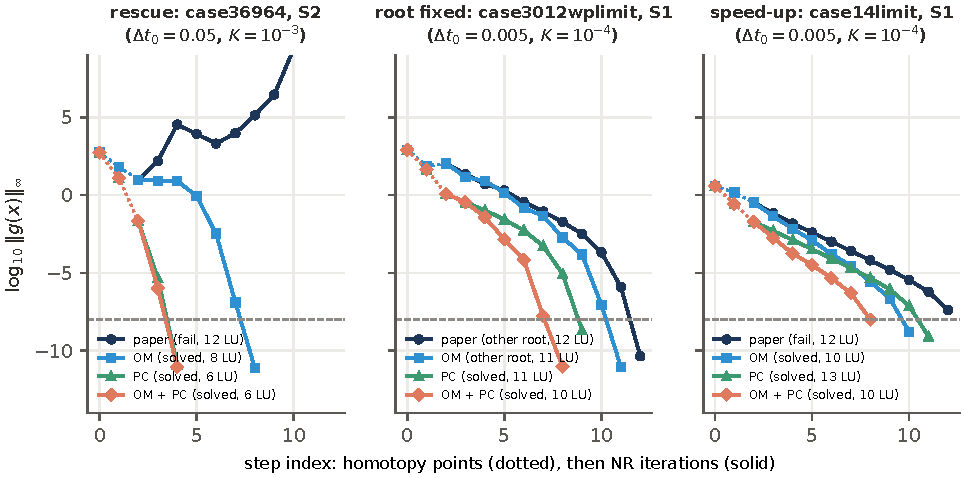
\includegraphics[width=\textwidth]{figures/rescues.pdf}
\caption[A rescue, a root fix and a speed-up]{Mismatch along the path (dotted) and through NR (solid) for
three runs the paper's method does not solve, one of each kind. The legend gives the outcome (solved means
the reference solution) and the LU count. Dashed line: tolerance $10^{-8}$.}
\label{fig:rescues}
\end{figure}

\Cref{fig:adaptive} shows how the adaptive rule handles \code{case6748}. The direct jump from $t_1$ to $t=1$
lands exactly where the paper's fixed path does, at a mismatch of 1798, and is rejected; the rule halves the
step six times, finds that only a step of 0.0155 reduces the mismatch, and from there doubles its way to
$t=1$ in eight points. NR then needs three iterations. The whole solve costs 18 LUs---three times the paper's
method on an easy system, but the paper's method does not solve this one at all.

\begin{figure}[!htbp]
\centering
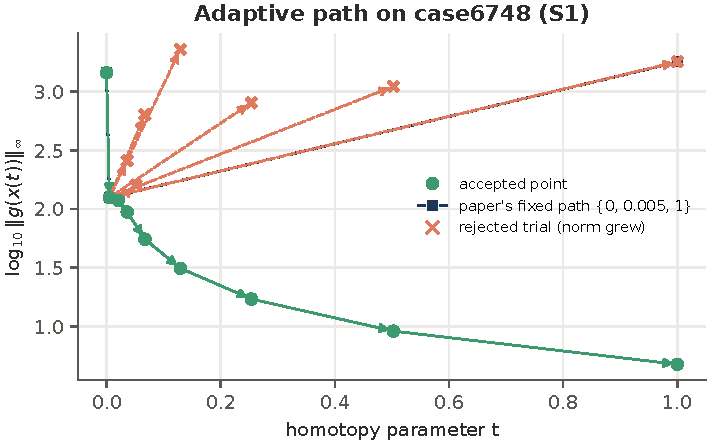
\includegraphics[width=0.72\textwidth]{figures/adaptive_path.pdf}
\caption[The adaptive path on case6748]{Every step the adaptive rule (with the multiplier) tries on
\code{case6748}, setting S1. Green: accepted steps; orange: rejected trials, which still cost an LU each. The
navy square path is the paper's fixed path, which ends at the same point as the first rejected jump.}
\label{fig:adaptive}
\end{figure}

% ============================================================================ 9 PROPOSAL STUDIES
\section{The Proposal's Numerical Studies}\label{sec:proposal}

Our proposal presentation stated four numerical studies around the paper's central parameter, the shift
$\delta=K/\Delta t_0$ of the first step. Like the modifications of \cref{sec:mods}, they build on the paper's
method, so they live in the same \code{improvements} package and run through the same command. Each has
its own experiment (exp12--exp15) and can be run on any system:
\begin{codebox}{Listing 3 \quad The proposal studies from the command line}
\begin{lstlisting}[language=bash,basicstyle=\ttfamily\footnotesize,numbers=none,columns=fullflexible]
python -m improvements spectrum case18482   # power method and inverse iteration
python -m improvements feasibility case6024 # (K, dt0) map as text
python -m improvements tune case6024        # golden-section search for delta and dt0
python -m improvements scratch case_ACTIVSg500limit --refiner FDXB   # our own LU
\end{lstlisting}
\end{codebox}

\subsection{The spectrum of the flat-start Jacobian}
The first BE step solves with $J+\delta I$ (\cref{eq:shift}), whose eigenvalues are those of $J$ moved by
$\delta$. How large $\delta$ must be depends on how close the eigenvalues of $J(\xo)$ come to zero.

\paragraph{Method} The largest eigenvalue modulus comes from the power method. $J$ is not symmetric and its
dominant eigenvalues can come as a complex pair or a $\pm\lambda$ pair, for which the plain iteration
oscillates, so we iterate with $J$ applied twice and take $\sqrt{\norm{J^2x}/\norm{x}}$. The smallest
modulus comes from inverse iteration: the same power method applied to $(J-\sigma I)^{-1}$, using one sparse
LU of $J-\sigma I$ and then only triangular solves. With $\sigma=0$ it gives $|\lambda|_{\min}(J)$, and with
$\sigma=-\delta$ the smallest eigenvalue modulus of $J+\delta I$. ARPACK (\code{scipy.sparse.linalg.eigs}) is
used as an independent check. The ratio $|\lambda|_{\max}/|\lambda|_{\min}$ is a lower bound on the
2-norm condition number of $J$.

\paragraph{What it shows} On the twelve ill-conditioned systems $|\lambda|_{\min}(J)$ is $4\times10^{-4}$ to
$6\times10^{-3}$, while $|\lambda|_{\max}$ is $2.7\times10^{4}$ to $5.2\times10^{4}$, so the eigenvalue ratio
reaches $1.2\times10^{8}$ (\code{case109272}). The paper's $\delta=0.02$ lifts the smallest eigenvalue to about
0.02 and cuts the ratio to $1.1$--$2.3\times10^{6}$ on all twelve, a factor of 4 to 50 (\cref{fig:spectrum}).
On most limit cases the smallest eigenvalue is already 0.01 to 1.9, as large as the shift or larger, so the
shift hardly changes anything---which is why the paper's method behaves like plain NR on those systems. The
two exceptions are the limit cases built from the two largest PEGASE grids, \code{case9241pegaselimit} and
\code{case13659pegaselimit}, whose spectrum looks like that of the ill-conditioned replicas.

\begin{figure}[!htbp]
\centering
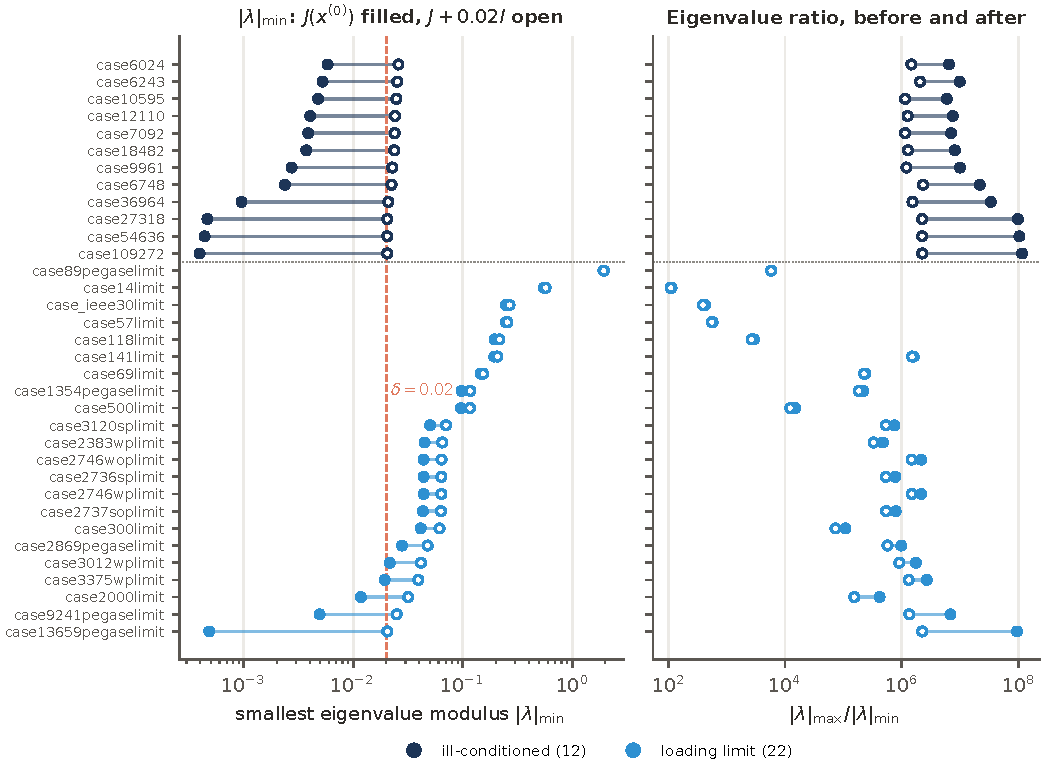
\includegraphics[width=\textwidth]{figures/spectrum.pdf}
\caption[Spectrum of the flat-start Jacobian]{Smallest eigenvalue modulus (left) and the ratio
$|\lambda|_{\max}/|\lambda|_{\min}$ (right) of $J(\xo)$ (filled) and of the shifted matrix $J+0.02I$ of the
first BE step (open), for all 34 systems. The shift only matters where $|\lambda|_{\min}$ is below
$\delta$: on the ill-conditioned systems and the two large PEGASE limit cases.}
\label{fig:spectrum}
\end{figure}

\paragraph{How accurate the iterations are} Inverse iteration agrees with ARPACK to four digits on 33 of
the 34 systems (on \code{case57limit} it is 8\% off). The power method is less reliable: it is off by up to
19\% (\code{case10595}), and all its large errors are on the networks built from copies of the same grid.
There every copy contributes an eigenvalue of almost the same modulus, so the ratio of the two largest
moduli is close to one and the power method, whose error falls like that ratio to the power of the
iteration count, has not converged after its 500 iterations. The textbook convergence condition of the power
method is violated by construction of the test systems.

\subsection{\texorpdfstring{Where the method works in the $(K,\Delta t_0)$ plane}{Where the method works in the (K, dt0) plane}}
The paper tries three $(\Delta t_0,K)$ pairs. \Cref{fig:feasibility} runs its method (BE on
$\{0,\Delta t_0,1\}$, then NR) on an $8\times11$ grid, $\Delta t_0$ from 0.001 to 0.2 and $K$ from
$10^{-6}$ to $10^{-1}$, for four systems, and marks whether each run reaches the reference solution, another
root, or fails. Lines of constant $\delta$ are diagonals of these maps.

\begin{figure}[!htbp]
\centering
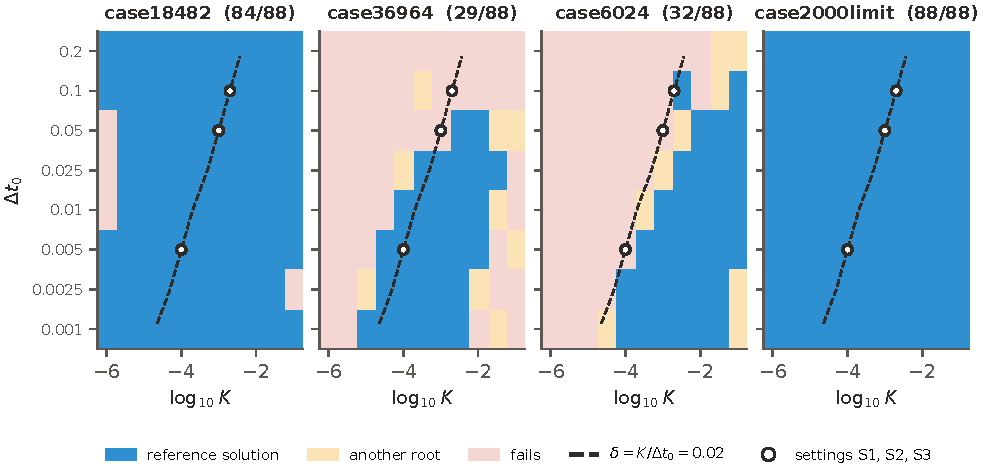
\includegraphics[width=\textwidth]{figures/feasibility.pdf}
\caption[Feasible region in the $(K,\Delta t_0)$ plane]{Outcome of the paper's method on a grid of $K$ and
$\Delta t_0$ (the title gives the cells that reach the reference solution). Dashed: $\delta=0.02$, the
paper's shift. Circles: the settings S1, S2 and S3 of the modification study.}
\label{fig:feasibility}
\end{figure}

The method works in a band along the diagonals $\delta=\text{const}$, which confirms that $\delta$ and not
$K$ or $\Delta t_0$ alone is the parameter that matters (\cref{sec:firststep}). How wide the band is
depends on the system. For \code{case18482} and \code{case2000limit} almost the whole grid works. For
\code{case36964} only 29 of 88 cells work, and no cell with $\Delta t_0=0.1$ or 0.2 works: this is why the
paper found that $\Delta t_0=0.1$ with $K=0.002$ fails even though $\delta$ is unchanged
(\cref{sec:audit}). For \code{case6024} the band lies at larger shifts, $\delta$ from 0.03 to 32, and the
paper's $\delta=0.02$ line runs along its edge, where runs reach other roots; the paper's own setting fails
there. Both of the systems with a narrow band have nine cells that converge to another root, mostly at the
edges of the band.

\subsection{\texorpdfstring{Tuning $\delta$ by golden-section search}{Tuning delta by golden-section search}}
\paragraph{Method} The objective is the total LU count of the paper's method, with a failed run costing 50,
plus a small tie-break $0.1\log_{10}\ninf{g(x(1))}$ so that the search can move inside a plateau of equal
integer counts. Golden-section search runs first over $\log_{10}\delta\in[-4,1]$ at $\Delta t_0=0.005$, then
over $\log_{10}\Delta t_0\in[-3,-0.5]$ with that $\delta$, each to a bracket of 0.05 decades, for 21 solves
per system in total. The objective is piecewise constant and not unimodal, so the search returns the best
point it has seen rather than the last bracket.

\paragraph{What it shows} The tuned values tell a different story from the paper's single $\delta$. For
\code{case27318}, \code{case54636} and \code{case109272} the search lands at $\delta=0.025$, close to the
paper's 0.02; the paper's choice suits its own systems. On the other ill-conditioned systems it prefers
$\delta=1$ to 5, fifty times larger, and on most limit cases it runs to the lower end of the interval,
because there $\delta$ hardly matters (\cref{fig:tuning}). At the tuned point 32 of the 34 systems are
solved; the two that are not are \code{case14limit} and \code{case2736splimit}, which need 11 NR iterations
whatever the start.

We then fitted two rules on the paper's nine systems and tested them on the other 25 (\cref{tab:tuning}): a
fixed $\delta$, the geometric mean of the tuned values, and a \emph{spectral rule} $\delta=c\,|\lambda|_{\min}$,
with $c$ the geometric mean of $\delta/|\lambda|_{\min}$, which costs one extra LU for the inverse iteration.
The fixed rule gives $\delta=0.011$ and behaves like the paper's 0.02. The spectral rule does not work: on
the ill-conditioned systems the tuned $\delta$ is 54 to 819 times $|\lambda|_{\min}$, so no single factor fits,
and on the limit cases $\delta$ barely matters. It loses four of the nine training systems. Searching each
system separately solves four more test systems than the paper's $\delta$, but the search costs 21 solves,
far more than it saves.

\begin{figure}[!htbp]
\centering
\begin{minipage}[c]{0.55\textwidth}
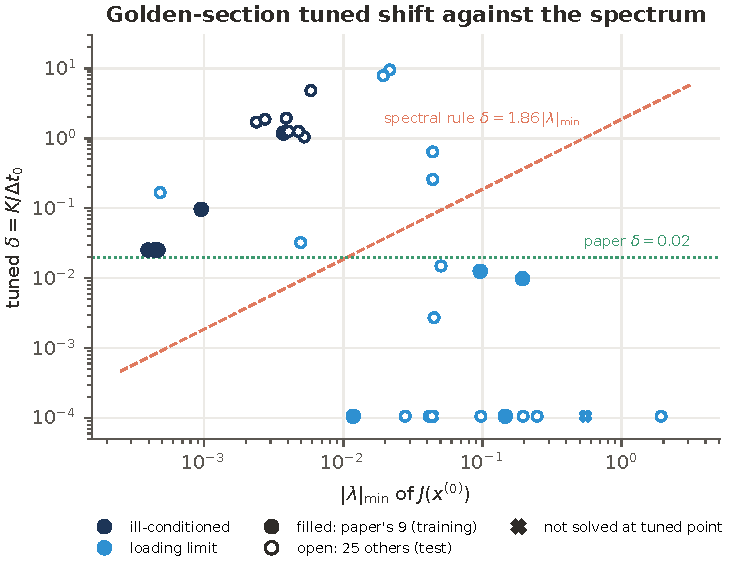
\includegraphics[width=\linewidth]{figures/tuning.pdf}
\end{minipage}\hfill
\begin{minipage}[c]{0.42\textwidth}
\caption[Tuned shift against the spectrum]{Golden-section tuned $\delta$ against $|\lambda|_{\min}(J(\xo))$ for
all 34 systems. Points at $10^{-4}$ are systems where the search ran to the lower end because $\delta$ does
not matter. A spectral rule would put the points on a line of slope one; they are nowhere near one.}
\label{fig:tuning}
\end{minipage}
\end{figure}

\begin{table}[!htbp]
\centering
\caption[Choosing $\delta$: rules fitted on the paper's systems]{Choosing $\delta$ without a search: rules
fitted on the paper's nine systems, tested on the other 25 ($\Delta t_0=0.005$ except for the per-system
search). Mean LUs are over the solved systems and exclude the cost of the search itself.}
\label{tab:tuning}
\small
\begin{tabular}{@{}l c r c r@{}}
\toprule
\headrow \thead{How $\delta$ is chosen} & \thead{Solved, training} & \thead{LUs} & \thead{Solved, test} & \thead{LUs} \\
\midrule
paper, $\delta=0.02$ & 9 of 9 & 5.00 & 19 of 25 & 9.47 \\
fixed rule, $\delta=0.011$ & 9 of 9 & 5.11 & 19 of 25 & 9.53 \\
spectral rule, $\delta=1.86\,|\lambda|_{\min}$ & \textbf{5 of 9} & 5.20 & 20 of 25 & 11.00 \\
golden search per system (21 solves) & 9 of 9 & 4.89 & \textbf{23 of 25} & 9.13 \\
\bottomrule
\end{tabular}
\end{table}

\subsection{Linear solvers written from scratch}\label{sec:ownlu}
\paragraph{Method} \code{improvements/gauss.py} implements Gauss elimination with partial pivoting and
back substitution, and a Doolittle LU factorization with partial pivoting, $PA=LU$, with $L$ (unit diagonal)
and $U$ stored in one array and the row permutation as an index vector, followed by forward and back
substitution. The row updates are vectorised, but both methods work on dense arrays and cost
$\mathcal{O}(n^3)$. \code{improvements/scratch.py} repeats the paper's BE path, NR and FDXB with every linear
system solved this way, step for step as in \code{dynhomotopy}, so the two can be compared one to one.

\paragraph{What it shows} On the tutorial and on the limit cases of 69 to 2{,}000 buses, our LU gives
exactly the same iteration counts as SuperLU and the same solution to $5\times10^{-12}$
(\cref{tab:ownlu}). The time shows why the paper's systems need a sparse solver: NR on
\code{case2000limit} takes \SI{424}{s} with our LU against \SI{0.04}{s} with SuperLU. From 943 to 3{,}607
unknowns the time grows 123-fold, more than the $3.8^3=56$ of pure $\mathcal{O}(n^3)$ scaling, presumably
because the larger matrices no longer fit in cache. The dense Jacobian of \code{case109272} alone would need
$185{,}807^2\times8$ bytes, about \SI{276}{GB}. Reuse of the factors matters as well: for 20 right-hand sides
with one $400\times400$ matrix, one LU plus 20 pairs of triangular solves takes \SI{0.054}{s} against
\SI{0.747}{s} for 20 Gauss eliminations, 14 times less, which is why FDXB factorises $B'$ and $B''$ once.

\begin{table}[!htbp]
\centering
\caption[The paper's method with our own LU]{The paper's method (BE path $\{0,0.005,1\}$, $K=10^{-4}$) with
SciPy's sparse LU and with our dense LU with partial pivoting: iterations of the refiner, largest difference
in the solution, and run time.}
\label{tab:ownlu}
\small
\begin{tabular}{@{}l l r r r r r@{}}
\toprule
\headrow \thead{System} & \thead{Refiner} & \thead{Its SuperLU} & \thead{Its ours} & \thead{max $|\Delta x|$} & \thead{SuperLU (s)} & \thead{Ours (s)} \\
\midrule
tutorial (Sec.~3.3)  & NR   & 9  & 9  & 0             & 0.002 & 0.002 \\
\code{case69limit}   & NR   & 1  & 1  & $3.6\times10^{-13}$ & 0.004 & 0.011 \\
                     & FDXB & 8  & 8  & $1.6\times10^{-13}$ & 0.004 & 0.010 \\
\code{case141limit}  & NR   & 1  & 1  & $9.7\times10^{-14}$ & 0.005 & 0.039 \\
                     & FDXB & 8  & 8  & $4.7\times10^{-12}$ & 0.004 & 0.032 \\
\code{case500limit}  & NR   & 2  & 2  & $9.8\times10^{-15}$ & 0.010 & 3.45 \\
                     & FDXB & 13 & 13 & $1.2\times10^{-14}$ & 0.008 & 1.71 \\
\code{case2000limit} & NR   & 3  & 3  & $4.3\times10^{-14}$ & 0.040 & 424.1 \\
                     & FDXB & 22 & 22 & $6.2\times10^{-14}$ & 0.029 & 100.8 \\
\bottomrule
\end{tabular}
\end{table}

\begin{finding}[What the numerical studies establish.]
The shift $\delta$ matters exactly where the spectrum says it should: on systems whose flat-start Jacobian has
eigenvalues below $\delta$. There the method works in a band of constant $\delta$ whose position and width
depend on the system, and the paper's $\delta=0.02$ sits well inside the band for some systems and on its
edge for others. Neither a fixed value nor a multiple of $|\lambda|_{\min}$ predicts the best $\delta$; a
per-system search does, but costs more than it saves. This is why the corrector, which makes more settings
work (\cref{sec:modresults}) instead of looking for a better one, is worth more than tuning $\delta$.
\end{finding}

% ============================================================================ 10 FAILURE ANALYSIS
\section{Failure Analysis}\label{sec:failure}

This section collects every failure---of the paper's integrators, of the modifications that did not work,
of the proposal ideas that did not deliver, and of our own measurements---and explains each from the
equations where we can. Where an explanation is our interpretation rather than something we measured
directly, we say so.

\subsection{Why explicit schemes fail on the first step}
Forward Euler at $t=0$ inverts $G_x=KI$ and therefore steps by $-(\Delta t_0/K)\,g(\xo)$
(\cref{sec:firststep}). The step is proportional to the mismatch and blind to the network, and the
ill-conditioned systems start with mismatches of 200--530. RK2 evaluates its second slope at that FE point,
so it inherits the damage. This is not a question of step size: making $\Delta t_0/K$ small enough to be
safe makes the step useless, which is why the paper and our code always take the first step with BE.

\subsection{Why explicit schemes still fail with large later steps}
After $t_1$, an explicit step to $t=1$ uses $G_x=t_1J+(1-t_1)KI$ evaluated at $t_1=0.005$, a matrix
that is still dominated by $KI$ in every direction where $J$ is small, so the same blindness returns in
those directions. BE instead uses $G_x$ at $t=1$, that is $J$ itself (\cref{sec:firststep}). The ODE is stiff
in exactly the sense of~\cite{hairer1996}: its fast modes, with time scale $K/\lambda(J)$, are far faster
than the path, and only an implicit method can step over them. More path points help FE and RK2 (Table 5,
\cref{fig:sec44}) because they reduce the step at which the stale $G_x$ is used. The spectrum makes the
stiffness concrete: with $|\lambda|$ from $4\times10^{-4}$ to $5\times10^{4}$ (\cref{fig:spectrum}), the time
scales $K/|\lambda|$ of the modes span eight orders of magnitude.

\subsection{Why RK4 fails, and why higher order does not pay under error control}
With fixed steps RK4 solves 13 of 170 runs. It is explicit, and its intermediate stages sit at
$t+\Delta t/2$ and $t+\Delta t$ using slopes computed from explicit predictions; with $\Delta t\approx1$ each
stage has the FE failure mode above, and higher order only multiplies the number of bad evaluations (four
LUs per step). Order of accuracy is irrelevant when the step is outside the stability region.

Richardson control repairs this by shrinking the step until the estimate is small, and then RK4 does solve
145 runs---but the step it can take is set by stability, not by accuracy, so it is no larger than FE's, and
each attempt now costs twelve LUs (three steps of four stages). That is why it needs 87 LUs in S1 against 37
for FE and 10.6 for BE, and why the paper's preference for BE survives a fair, error-controlled comparison.
Richardson with RK4 is also the only Richardson configuration that loses more than one run the paper's method
solves (nine): on six of them it converges to another root, and on three NR fails from where the path
ends. More stages do not make the path more faithful when the step is limited by stability.

\subsection{Why refining backward Euler makes it worse}
The paper suggests after its eq.~(19) that more fixed-point iterations could improve BE. BE-chord loses 47
runs and lands on another root 24 times. The reason is the contraction condition of the iteration it performs,
\[
  \hat x \mapsto x_k - \Delta t\,G_x(x_k,t_{k+1})^{-1}\,G_t(\hat x),
  \qquad
  \frac{\partial}{\partial \hat x} = -\Delta t\,G_x(x_k,t_{k+1})^{-1}\bigl(J(\hat x)-KI\bigr).
\]
On the last step $t_{k+1}=1$, so $G_x=J(x_k)$, and when $J(\hat x)\approx J(x_k)$ the iteration matrix is
close to $-\Delta t\,I$ with $\Delta t=0.995$: its spectral radius is about one, so the iteration does not
contract---it oscillates. The first iterate is useful (it is the near-Newton step of \cref{sec:firststep});
the second and third move back and forth around it. For small steps the same iteration would contract,
which is presumably the regime the paper had in mind. (This is our analysis of why the iteration drifts;
we measured the outcome, not the spectral radius.)

\subsection{Why the Newton homotopy fails}
The Newton homotopy $G=g(x)-(1-t)g(\xo)$ has $G_x=J(x)$ at every $t$: no $KI$ term. Its BE first step is
$\Delta x=-\Delta t_0\,J(\xo)^{-1}g(\xo)$, a plain Newton step shrunk to 0.5\%, with the flat-start Jacobian
unregularised. It solves 75 of 170 runs; in setting S1 it fails on every ill-conditioned system except
\code{case27318} and \code{case54636}, and on \code{case109272} it converges to another root. This is the
clearest evidence in the project for the paper's central idea: the useful ingredient is the $KI$ shift of
the Jacobian, not homotopy continuation as such.

\subsection{Why the scaled homotopy changes little}
Scaling the shift by $D=|\mathrm{diag}\,J(\xo)|$ gives exactly the paper's result in S1, S2 and S4, loses one
run in S3 (\code{case27318}), and in S5 corrects the wrong roots of \code{case27318}, \code{case54636} and
\code{case109272}: 129 solved in total, against 127. Our interpretation of why it does not help more: $D$ is
normalised to mean one, so equations with a small Jacobian diagonal get a \emph{smaller} shift than
before---and those weakly coupled equations are exactly the ones the shift is there to protect. A scaling
that raises the shift where the diagonal is weak would be the natural next try.

\subsection{Why part of the corrector's gain is accounting}\label{sec:pc-accounting}
At $t=1$ the homotopy is $G(x,1)=g(x)$ and $G_x(x,1)=J(x)$, so the corrector's last step is \emph{exactly}
one NR step, taken before the 10-iteration budget starts counting. Ten of the corrector's 25 gains are the
budget-edge speed-ups of \cref{sec:rescue}. On \code{case14limit} and \code{case2736splimit} the corrector
solves with 13 LUs---exactly what the paper's method needs if it is simply allowed its eleventh NR iteration
($2+11$). So on those two systems the corrector is not cheaper and not more robust; it only moves one
iteration outside the count. The other 15 gains are real: its two rescues (\code{case36964} in S2 and S3,
where at 6 LUs it is the cheapest solver we have) and its 13 root fixes, which no count of iterations can
explain. The LU metric makes the difference visible; a pure success count hides it.

\subsection{Where adaptive steps lose}\label{sec:adaptive-fail}
The adaptive rule accepts a step only if $\ninf{g}$ decreases. But the homotopy path does not promise that:
on the path, $g(x(t))=-\tfrac{1-t}{t}K(x(t)-\xo)$, whose norm need not fall monotonically. So the rule can
reject perfectly good steps. That is what happens on \code{case2000limit} in S1: the paper's direct jump
works with 5 LUs, the adaptive rule rejects it and spends 14. It also explains the one run adaptive loses,
\code{case2383wplimit} with strong $K$ (S5), where it runs out of halvings. Measuring progress by
$\norm{G(x,t)}$ instead of $\norm{g(x)}$ would respect the path; we did not test it. Richardson control
avoids the problem because it measures the integration error, not the mismatch---at a higher price per step.

\subsection{Why Richardson control still finds wrong roots}
Richardson with BE lands on another root 9 times, the corrector twice. The error estimate compares two
integrations with each other; it does not measure how far either is from the homotopy curve, and with the
tolerance of 0.5 that we chose (so that paths stay cheap) both can drift together towards another branch.
The corrector measures exactly that distance, $G(x,t)$, and pulls the state back. (This is our explanation;
we did not vary the tolerance.) Combining the two would be the obvious next step, but it would add one more LU to each
of the three steps of every attempt.

\subsection{\texorpdfstring{Why no simple rule predicts $\delta$}{Why no simple rule predicts delta}}
The spectral rule assumes that the right shift is proportional to $|\lambda|_{\min}(J)$. The feasibility maps
show why it cannot be: the band of working $\delta$ lies at 0.006--3 for \code{case36964} and at 0.03--32 for
\code{case6024}, although their smallest eigenvalues differ by a factor of six in the other direction
($10^{-3}$ against $6\times10^{-3}$). What decides whether the first step lands in NR's region of
convergence depends on the whole nonlinear problem, not on one eigenvalue of the linearisation at the start.
The smallest eigenvalue does say something useful, but only as a yes/no test: if it is well above
$0.02$, $\delta$ does not matter.

\subsection{The seven runs nothing solves}\label{sec:nothing}
Seven runs fail under every configuration, all in setting S4, with the weak $K=10^{-5}$ ($\delta=0.002$, ten
times less regularisation than the paper's): \code{case36964}, \code{case6024}, \code{case6243},
\code{case6748}, \code{case9961}, \code{case3012wplimit} and \code{case3375wplimit}. S4 is the setting where
the paper's method drops to 18 of 34. Richardson control with an explicit step rule gets furthest (27 of 34),
but no switch fully compensates for too small a shift.

\subsection{Failures of our own measurement}
Three measurement problems were ours, not the method's.
\begin{itemize}
  \item \textbf{Counting convergence as success.} Our first version of the modification study counted a run
        as solved when NR converged. Under that criterion the paper's method solved 141 runs and the
        multiplier looked like the best single change. Checking the voltages against the reference
        operating point showed that 14 of the paper's converged runs, and 12 of the multiplier's, reach
        another root, and it reversed the ranking of the multiplier and the corrector. Every result in this
        report uses the stricter criterion.
  \item \textbf{Budget-edge systems.} The criterion ``NR within 10 iterations'' is blunt on systems that
        need exactly 11, which is why \cref{sec:rescue} re-runs every gained case with 30 iterations before
        calling it a rescue.
  \item \textbf{Wall-clock noise.} Times on a laptop depend on its load; we report medians of seven runs,
        compare only percentages with the paper, and base all our own cost conclusions on LU counts.
\end{itemize}

% ============================================================================ 11 DISCUSSION
\section{Discussion}\label{sec:discussion}

\subsection{Strengths}
The reproduction is close and fully traceable: every number in this report comes from a script in the
repository that prints our value next to the paper's, and the tests check the building blocks against
independent computations before any comparison. The analysis of \cref{sec:firststep}, that the paper's
method is a shifted Newton step followed by a near-Newton step, turns an empirical recommendation into an
explanation, and it predicted which of our modifications would work: the ones that improve the Newton stages
(corrector, multiplier) helped, and the one that removes the shift (Newton homotopy) failed. The
modification study is a controlled experiment on 34 systems, 25 of them unseen by the paper, with a
machine-independent cost measure; it checks that each run reaches the intended solution, and it separates
rescues, root fixes and speed-ups. The proposal studies connect the method to the numerical analysis behind
it: the spectrum explains where the shift matters, the feasibility maps show that $\delta$ is the right
parameter, and our own LU confirms the linear algebra independently of SciPy.

\subsection{Limitations}
\begin{itemize}
  \item The test bed is two Zenodo records. The ill-conditioned systems are replicas of a few base networks,
        so 12 systems carry less independent evidence than 12 unrelated grids would.
  \item The reference operating point is a convention: the solution NR reaches from the stored initial
        guess. We did not study whether the other roots are physically meaningful operating points.
  \item Only paths $\{0,\Delta t_0,1\}$ were used for the modification study; the modifications were not
        tested on the multi-point paths of the paper's Tables 5 and 6.
  \item The Richardson tolerance (0.5) and the golden-section brackets were set once and not tuned; the
        feasibility maps cover four systems.
  \item Our GSH-NR is a reconstruction from a verbal description, so the comparison with it is weaker than
        the rest.
  \item Timings are Python on a laptop and are noisy; they are reported but not relied on.
\end{itemize}

\subsection{Future work}\label{sec:future}
\begin{itemize}
  \item \textbf{Corrector plus error control.} Richardson control rescues the most divergent runs and the
        corrector fixes the most wrong roots; a Richardson path with a corrector after each accepted point
        would try to get both.
  \item \textbf{Cheaper error estimates.} An embedded pair, or reusing one LU for the three steps of each
        attempt, would cut the cost of Richardson control by up to a factor of three.
  \item \textbf{A path-aware acceptance test} for adaptive steps, based on $\norm{G(x,t)}$ rather than
        $\norm{g(x)}$ (\cref{sec:adaptive-fail}).
  \item \textbf{A scaling that raises the shift on weak equations}, the opposite of our scaled homotopy.
  \item \textbf{A sparse LU from scratch}, with a fill-reducing ordering, to close the gap between our dense
        solver and SuperLU and run the whole pipeline on our own linear algebra.
\end{itemize}

% ============================================================================ 12 CONCLUSION
\section{Conclusion}\label{sec:conclusion}
We set out to rebuild a published method for starting Newton--Raphson on ill-conditioned power grids and to
see how far it could be trusted and pushed. It reproduces: on all five ill-conditioned grids of up to
109{,}272 buses, NR from the flat start fails, and a two-point backward-Euler homotopy turns that into a
four-iteration solve, with our numbers matching the paper's across 28 orders of magnitude. It is also
simpler than its derivation suggests. With the paper's parameters, the first backward-Euler step is a
Newton step on a Jacobian shifted by $\delta=K/\Delta t_0$, and the second is almost a plain Newton step;
the implicit scheme wins because it is the only one that uses the real Jacobian where it matters.

On a test bed four times the size of the paper's, one question turned out to matter more than any other:
which solution does a converged run reach? The paper's method converges on 141 of 170 runs but reaches the
intended operating point on 127. A Newton corrector after every path step raises that to 152, loses nothing,
and cuts the wrong-root runs from 14 to 2; with Iwamoto's optimal multiplier added it does so with 7\% fewer
LU factorizations than the paper's method, and this is the configuration we recommend. Richardson error
control of the steps solves systems nothing else solves, at 18--30\% more factorizations, and confirms under
fair conditions that backward Euler is the right integrator. Four other ideas failed, each for a reason in
the equations: RK4 is explicit, extra fixed-point iterations do not contract at a step of one, a scaled shift
weakens the equations that need it, and a homotopy without the shift does not work at all.

The proposal's studies explain the parameter behind all of this. The shift matters where the flat-start
Jacobian has eigenvalues below it, the method works in a band of constant $\delta$ whose position differs from
system to system, and neither a fixed value nor a spectral rule predicts the best $\delta$. Our own Gauss
elimination and LU reproduce every iterate, and show at 424 seconds for a 2{,}000-bus system why a sparse
solver is not optional.

The lesson we take from the project is that the choice of what to count decides the conclusions. Counting LU
factorizations instead of seconds, asking whether a ``solved'' run was rescued or merely hurried, and above
all checking that it reached the right solution each changed a conclusion that a plain success count would
have got wrong.

% ============================================================================ REFERENCES
\clearpage
\begin{thebibliography}{99}\small
\setlength{\itemsep}{2pt}
\bibitem{lima2024} A.~Lima-Silva and F.~D.~Freitas, ``Exploring a dynamic homotopy technique to enhance the
  convergence of classical power flow iterative solvers in ill-conditioned power system models,''
  \emph{Energies}, vol.~17, no.~18, art.~4642, 2024. doi:10.3390/en17184642.
\bibitem{lima2024ijepes} A.~Lima-Silva and F.~D.~Freitas, ``Dynamical homotopy transient-based technique to
  improve the convergence of ill-posed power flow problem,'' \emph{Int.\ J.\ Electr.\ Power Energy Syst.},
  vol.~155, art.~109436, 2024.
\bibitem{freitas2022} F.~D.~Freitas and A.~L.~Silva, ``Flat start guess homotopy-based power flow method guided
  by fictitious network compensation control,'' \emph{Int.\ J.\ Electr.\ Power Energy Syst.}, vol.~142,
  art.~108311, 2022.
\bibitem{freitas2023} F.~D.~Freitas and L.~N.~de~Oliveira, ``Conditioning step on the initial estimate when
  solving ill-conditioned power flow problems,'' \emph{Int.\ J.\ Electr.\ Power Energy Syst.}, vol.~146,
  art.~108772, 2023.
\bibitem{iwamoto1981} S.~Iwamoto and Y.~Tamura, ``A load flow calculation method for ill-conditioned power
  systems,'' \emph{IEEE Trans.\ Power App.\ Syst.}, vol.~PAS-100, no.~4, pp.~1736--1743, 1981.
\bibitem{milano2009} F.~Milano, ``Continuous Newton's method for power flow analysis,'' \emph{IEEE Trans.\
  Power Syst.}, vol.~24, no.~1, pp.~50--57, 2009.
\bibitem{tinney1967} W.~F.~Tinney and C.~E.~Hart, ``Power flow solution by Newton's method,'' \emph{IEEE
  Trans.\ Power App.\ Syst.}, vol.~PAS-86, no.~11, pp.~1449--1460, 1967.
\bibitem{stott1974} B.~Stott and O.~Alsac, ``Fast decoupled load flow,'' \emph{IEEE Trans.\ Power App.\ Syst.},
  vol.~PAS-93, no.~3, pp.~859--869, 1974.
\bibitem{vanamerongen1989} R.~A.~M.~van~Amerongen, ``A general-purpose version of the fast decoupled load
  flow,'' \emph{IEEE Trans.\ Power Syst.}, vol.~4, no.~2, pp.~760--770, 1989.
\bibitem{matpower} R.~D.~Zimmerman, C.~E.~Murillo-S\'anchez and R.~J.~Thomas, ``MATPOWER: Steady-state
  operations, planning, and analysis tools for power systems research and education,'' \emph{IEEE Trans.\
  Power Syst.}, vol.~26, no.~1, pp.~12--19, 2011.
\bibitem{tostado2019ill} M.~Tostado-V\'eliz, S.~Kamel and F.~Jurado, \emph{Matpower ill-conditioned systems}
  (version 1), data set, Zenodo, record 3514739, 2019.
\bibitem{tostado2019limit} M.~Tostado-V\'eliz, S.~Kamel and F.~Jurado, \emph{Matpower limit cases}
  (version 1), data set, Zenodo, record 3491654, 2019.
\bibitem{pegase} S.~Fliscounakis, P.~Panciatici, F.~Capitanescu and L.~Wehenkel, ``Contingency ranking with
  respect to overloads in very large power systems taking into account uncertainty, preventive, and
  corrective actions,'' \emph{IEEE Trans.\ Power Syst.}, vol.~28, no.~4, pp.~4909--4917, 2013.
\bibitem{watson1989} L.~T.~Watson, ``Globally convergent homotopy methods: A tutorial,'' \emph{Appl.\ Math.\
  Comput.}, vol.~31, pp.~369--396, 1989.
\bibitem{allgower2003} E.~L.~Allgower and K.~Georg, \emph{Introduction to Numerical Continuation Methods},
  SIAM Classics in Applied Mathematics, vol.~45, 2003.
\bibitem{hairer1996} E.~Hairer and G.~Wanner, \emph{Solving Ordinary Differential Equations II: Stiff and
  Differential-Algebraic Problems}, 2nd ed., Springer, 1996.
\bibitem{levenberg1944} K.~Levenberg, ``A method for the solution of certain non-linear problems in least
  squares,'' \emph{Quart.\ Appl.\ Math.}, vol.~2, no.~2, pp.~164--168, 1944.
\bibitem{marquardt1963} D.~W.~Marquardt, ``An algorithm for least-squares estimation of nonlinear
  parameters,'' \emph{J.\ SIAM}, vol.~11, no.~2, pp.~431--441, 1963.
\bibitem{scipy} P.~Virtanen \emph{et al.}, ``SciPy 1.0: Fundamental algorithms for scientific computing in
  Python,'' \emph{Nature Methods}, vol.~17, pp.~261--272, 2020.
\bibitem{superlu} X.~S.~Li, ``An overview of SuperLU: Algorithms, implementation, and user interface,''
  \emph{ACM Trans.\ Math.\ Softw.}, vol.~31, no.~3, pp.~302--325, 2005.
\end{thebibliography}

% ============================================================================ APPENDICES
\clearpage
\appendix
\section{Reproducing This Report}\label{app:repro}
All results come from the repository. Test systems are downloaded from Zenodo on first use.
\begin{codebox}{Commands}
\begin{lstlisting}[language=bash,basicstyle=\ttfamily\footnotesize,numbers=none,columns=fullflexible]
pip install -r requirements.txt
python -m pytest tests                     # 24 tests
python run_all.py                          # every experiment (1-15)
python run_all.py --only 3 4               # selected experiments
python -m experiments.exp11_improvements --configs PC "OM + PC" richardson
python -m improvements --help              # any modification on any of the 34 systems
python -m improvements spectrum case18482   # any proposal study on any system
python report/scripts/figures_from_results.py   # report figures from results/tables
python report/scripts/figures_from_code.py      # report figures that call the solvers
\end{lstlisting}
\end{codebox}
Experiments 1 to 10 (the paper) take about an hour on a laptop; experiment 11 (17 configurations
$\times$ 170 runs) takes several hours. With \code{--configs}, experiment 11 runs only the named
configurations, always together with the paper's method, and writes its tables as
\code{improvements\_selected\_*}.

\begin{table}[h]
\centering
\caption[Map from each result to its script]{Map from each result of the paper, and of our own studies, to
the script that produces it and its output in \code{results/}.}
\label{tab:scripts}
\small
\begin{tabular}{@{}l l l@{}}
\toprule
\headrow \thead{Result} & \thead{Script} & \thead{Output} \\
\midrule
Figures 1 and 2 & \code{exp01\_tutorial.py} & \code{fig1*.png}, \code{fig2*.png} \\
Section 4.2.1 & \code{exp02\_first\_step.py} & \code{sec421\_first\_step.md} \\
Tables 2, 3, 4 & \code{exp03\_tables2to4.py} & \code{table2\_FE.md}, \code{table3\_RK2.md}, \code{table4\_BE.md} \\
Table 5 & \code{exp04\_table5.py} & \code{table5.md} \\
Section 4.4 & \code{exp05\_sec44\_pathways.py} & \code{sec44\_pathways.md} \\
Figure 3, Table 6 & \code{exp06\_fig3\_table6.py} & \code{fig3*.png}, \code{table6.md} \\
Figure 4 & \code{exp07\_fig4.py} & \code{fig4\_case109272\_states.png} \\
Figure 5 & \code{exp08\_fig5.py} & \code{fig5\_timestep\_sensitivity.png} \\
Table 7 & \code{exp09\_table7.py} & \code{table7.md}, \code{table7\_native\_base.md} \\
Table 8 & \code{exp10\_table8.py} & \code{table8.md} \\
Our modifications & \code{exp11\_improvements.py} & \code{improvements\_*.md} \\
Proposal: spectrum & \code{exp12\_spectrum.py} & \code{spectrum.md} \\
Proposal: $(K,\Delta t_0)$ maps & \code{exp13\_feasibility.py} & \code{feasibility.md}, \code{feasibility\_maps.png} \\
Proposal: tuning $\delta$ & \code{exp14\_tuning.py} & \code{tuning\_per\_case.md}, \code{tuning\_rules.md} \\
Proposal: own LU & \code{exp15\_scratch\_lu.py} & \code{scratch\_lu.md}, \code{gauss\_vs\_lu.md} \\
\bottomrule
\end{tabular}
\end{table}

\section{Full Tables}\label{app:tables}

\begin{table}[h]
\centering
\caption[Table 2 re-run: FE then NR]{Table 2 re-run: FE after a BE first step, path $\{0,0.005,0.01,0.51,1\}$,
$K=10^{-4}$ (our value above the paper's).}
\label{tab:fe}
\scriptsize
\setlength{\tabcolsep}{3pt}
\begin{tabular}{@{}l l r r r r r r r r l@{}}
\toprule
\headrow \thead{Case} & & \thead{$t{=}0$} & \thead{0.005} & \thead{0.01} & \thead{0.51} & \thead{1} & \thead{NR 1} & \thead{NR 2} & \thead{NR 3} & \thead{Result} \\
\midrule
\rows{generated/table2_rows.tex}
\bottomrule
\end{tabular}
\end{table}

\begin{table}[h]
\centering
\caption[Table 3 re-run: RK2 then NR]{Table 3 re-run: RK2 after a BE first step, same path and $K$.}
\label{tab:rk2}
\scriptsize
\setlength{\tabcolsep}{3pt}
\begin{tabular}{@{}l l r r r r r r r r l@{}}
\toprule
\headrow \thead{Case} & & \thead{$t{=}0$} & \thead{0.005} & \thead{0.01} & \thead{0.51} & \thead{1} & \thead{NR 1} & \thead{NR 2} & \thead{NR 3} & \thead{Result} \\
\midrule
\rows{generated/table3_rows.tex}
\bottomrule
\end{tabular}
\end{table}

\begin{table}[h]
\centering
\caption[Table 6 re-run: five-point paths, run time]{Table 6 re-run: median CPU time of seven runs as a
percentage of NR-MAT, with the NR iterations after the homotopy in brackets (ours / paper).}
\label{tab:t6}
\footnotesize
\setlength{\tabcolsep}{4pt}
\begin{tabular}{@{}l c l l l@{}}
\toprule
\headrow \thead{Method} & \thead{$t_3$} & \thead{\code{case109272}} & \thead{\code{case36964}} & \thead{\code{case2000limit}} \\
\midrule
NR-MAT & -- & 1.784\,s (100\%) & 0.797\,s (100\%) & 0.024\,s (100\%) \\
\midrule
FE  & 0.20 & 143\% [3] / 146\% & 185\% [7] / 178\% & 272\% [4] / 68\% \\
FE  & 0.25 & 143\% [3] / 145\% & \fail\ / \fail & 272\% [4] / 75\% \\
FE  & 0.30 & 164\% [4] / 170\% & 201\% [8] / 179\% & 239\% [3] / 72\% \\
RK2 & 0.20 & 225\% [4] / 230\% & \textbf{\fail\ / 232\%} & 341\% [3] / 82\% \\
RK2 & 0.25 & 224\% [4] / 226\% & 222\% [6] / 190\% & 340\% [3] / 84\% \\
RK2 & 0.30 & 224\% [4] / 237\% & 221\% [6] / 195\% & 342\% [3] / 73\% \\
BE  & 0.20 & 163\% [4] / 171\% & 168\% [6] / 144\% & 238\% [3] / 61\% \\
BE  & 0.25 & 164\% [4] / 171\% & 169\% [6] / 144\% & 237\% [3] / 81\% \\
BE  & 0.30 & 163\% [4] / 169\% & 170\% [6] / 148\% & 238\% [3] / 94\% \\
\bottomrule
\end{tabular}
\end{table}

\end{document}
